%-------------------------------------------------------------------------------
%                      Template Naskah Skripsi
%               	Berdasarkan format JTETI FT UGM
% 						(c) @gunturdputra 2014
%-------------------------------------------------------------------------------

%Template pembuatan naskah skripsi.
\documentclass{jtetiskripsi}

\renewcommand \thesection{\Alph{section}.}
\renewcommand \thesubsection{\arabic{subsection}.}

%Untuk prefiks pada daftar gambar dan tabel
\usepackage[titles]{tocloft}
\renewcommand\cftfigpresnum{Gambar\  }
\renewcommand\cfttabpresnum{Tabel\   }

%Untuk hyperlink dan table of content
\usepackage[hidelinks]{hyperref}
\newlength{\mylenf}
\settowidth{\mylenf}{\cftfigpresnum}
\setlength{\cftfignumwidth}{\dimexpr\mylenf+2em}
\setlength{\cfttabnumwidth}{\dimexpr\mylenf+2em}

%Untuk Bold Face pada Keterangan Gambar
\usepackage[labelfont=bf]{caption}

%Untuk caption dan subcaption
\usepackage{caption}
\usepackage{subcaption}

%pdf
\usepackage{pdfpages}

%table
\usepackage{graphics}

\usepackage{wrapfig}

%bibliography
\usepackage{natbib}

%equation
\usepackage{amsmath}
\allowdisplaybreaks

%algoritma
\usepackage{algorithm}
\usepackage{algpseudocode}

\usepackage{pdfpages}
\providecommand{\pgfsyspdfmark}[3]{}

%listing
\usepackage{listings, chngcntr}
\lstset
{ %Formatting for code in appendix
    language=Matlab,
    basicstyle=\footnotesize,
    numbers=left,
    stepnumber=1,
    showstringspaces=false,
    tabsize=1,
    breaklines=true,
    breakatwhitespace=false,
}
\renewcommand{\lstlistingname}{Kode}
\renewcommand{\lstlistlistingname}{DAFTAR KODE PEMROGRAMAN}
\AtBeginDocument{
    \counterwithout{lstlisting}{chapter}
}

\usepackage{longtable}
\usepackage{multirow}

\algdef{SE}[DOWHILE]{Do}{doWhile}{\algorithmicdo}[1]{\algorithmicwhile\ #1}

\makeatletter
\newenvironment{breakablealgorithm}
{
    \begin{center}
        \refstepcounter{algorithm}
        \renewcommand{\caption}[1]
        {
            \addcontentsline{loa}{algorithm}{\protect\numberline{\thealgorithm}##1}
            \parbox{\textwidth}
            % Makes a unbreakable block and can also be done by `minipage`.
            {
                \hrule height.8pt depth0pt \kern2pt
                {\raggedright\textbf{\fname@algorithm~\thealgorithm} ##1\par}
                \kern2pt\hrule\kern2pt
            }
        }
}
{
        \kern2pt\hrule\relax
    \end{center}
}
\makeatother

\usepackage{enumitem}

\usepackage{tocloft}
\setlength\cftparskip{-2pt}
\setlength\cftbeforechapskip{0pt}

\usepackage{draftwatermark}
\usepackage{tikz}
\SetWatermarkText{\centering{\tikz{\node[opacity=0.1]{
\includegraphics[width=0.8\paperwidth]{gambar/logo_unj_tanpa_text.png}};}}}
\SetWatermarkAngle{0}
\SetWatermarkScale{1}

%-----------------------------------------------------------------
%Disini awal masukan untuk data proposal skripsi
%-----------------------------------------------------------------
\titleind{Perbandingan Implementasi Algoritma-algoritma Pagerank pada Satu Mesin Komputer}

\fullname{Farhan Herdian Pradana}

\idnum{1313618030}

\degree{Sarjana Ilmu Komputer}

\yearsubmit{2023}

\program{Ilmu Komputer}

\dept{Ilmu Komputer}

\firstsupervisor{Muhammad Eka Suryana, M. Kom.}
\firstnip{198512232012121002}

\secondsupervisor{Med Irzal, M.Kom.}
\secondnip{197706152003121001}

%-----------------------------------------------------------------
%Disini akhir masukan untuk data proposal skripsi
%-----------------------------------------------------------------

\tolerance=1
\emergencystretch=\maxdimen
\hyphenpenalty=10000
\hbadness=10000

\begin{document}

\cover

%-----------------------------------------------------------------

%-----------------------------------------------------------------
%Disini akhir masukan untuk muka skripsi
%-----------------------------------------------------------------

\clearpage
\addcontentsline{toc}{chapter}{LEMBAR PERNYATAAN}
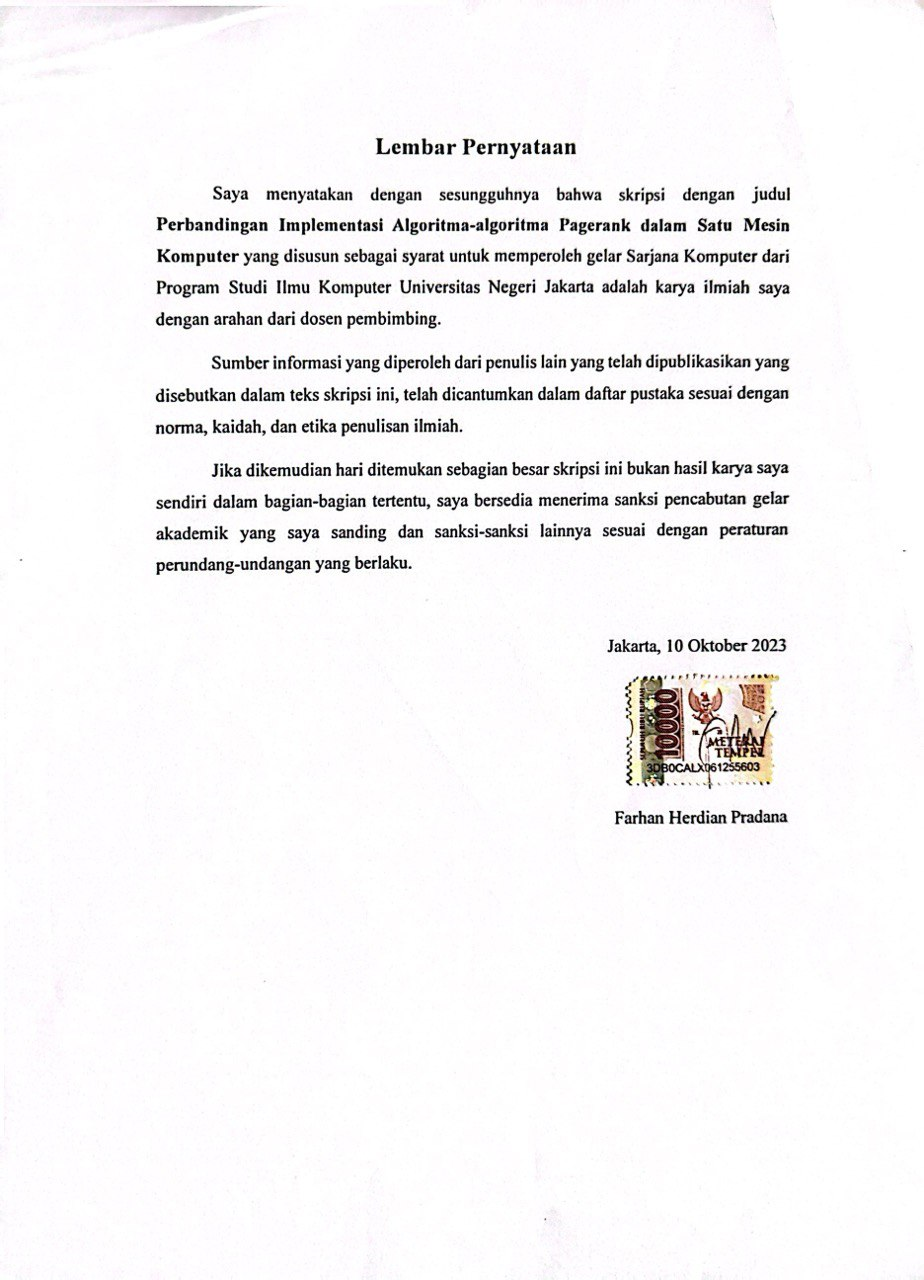
\includepdf{gambar/lembar_pernyataan.jpg}
\addcontentsline{toc}{chapter}{HALAMAN PERSEMBAHAN}
\chapter*{\centering{\large{HALAMAN PERSEMBAHAN}}}
\null\vfill
\begin{flushright}
\textit{Untuk Almh. Kak Irna}
\end{flushright}
\addcontentsline{toc}{chapter}{KATA PENGANTAR}
\chapter*{\centering{\large{KATA PENGANTAR}}}

Puji syukur terhadap ke hadirat tuhan Yang Maha Esa, yang telah memberikan nikmat, baik berupa kesehatan, waktu, maupun finansial sehingga dapat menyelesaikan skripsi yang berjudul \textbf{"Perbandingan Implementasi Algoritma-algoritma Pagerank pada Satu Mesin Komputer"}.

Selesainya skripsi ini tidak hanya berkat Penulis seorang melainkan juga ada pihak - pihak lain yang dengan tulus mau membantu Penulis dalam menyusun skripsi ini baik secara langsung dengan memberikan bimbingan, maupun dukungan finansial dan moril. Untuk itu izinkan Penulis mengucapkan banyak terima kasih kepada pihak-pihak berikut:

\begin{enumerate}[topsep=0pt, itemsep=-1ex]

	\item{Yth. Ibu Dr. Ria Arafiyah, M.Si selaku Koordinator Program Studi Ilmu Komputer.}
	\item{Yth. Bapak Muhammad Eka Suryana, M.Kom selaku Dosen Pembimbing I.}
	\item{Yth. Bapak Med Irzal, M.Kom selaku Dosen Pembimbing II.}
	\item{Seluruh staf dan dosen Program Studi Ilmu Komputer.}
	\item{Keluarga penulis.}
	\item{Teman-teman Program Studi Ilmu Komputer 2018.}
	
\end{enumerate}

Skripsi ini masih jauh dari kata sempurna dan Penulis sangat terbuka terhadap kritik dan masukan dari pembaca sehingga dapat menjadi bahan evaluasi Penulis dalam menulis skripsi dan tulisan sejenisnya. Semoga skripsi ini dapat memberikan manfaat bagi pembaca. 

\begin{flushright}
Jakarta, 10 Oktober 2023

\vspace{2cm}

Farhan Herdian Pradana
\end{flushright}
\addcontentsline{toc}{chapter}{ABSTRAK}
\chapter*{ABSTRAK}

\textbf{FARHAN HERDIAN PRADANA}. Perbandingan Implementasi Algoritma-algoritma Pagerank pada Satu Mesin Komputer. Skripsi. Fakultas Matematika dan Ilmu Pengetahuan Alam, Universitas Negeri Jakarta. 2023. Di bawah bimbingan Muhammad Eka Suryana, M. Kom, dan Med Irzal, M. Kom.

Algoritma Pagerank merupakan algoritma mengurutkan halaman web pada \textit{search engine} Google. Masalah pada Algoritma Pagerank adalah memerlukan memori utama yang cukup besar, dan tidak mungkin dilakukan pada satu mesin komputer dengan memori utama yang terbatas. Akan dicari algoritma alternatif dari Algoritma Pagerank Original buatan Google dengan membandingkannya pada algoritma-algoritma Pagerank dari penelitian lainnya dengan membandingkan kecepatan, penggunaan memori utama, dan kemiripan hasil. Penelitian dilakukan dengan melakukan pengkodean terhadap algoritma Pagerank Original, algoritma Distributed Pagerank Computation (DPC), algoritma Modified DPC (MDPC), dan algoritma Random Walker. Semua kode program dijalankan pada dataset dan dibandingkan kecepatan, penggunaan memori utama, dan kemiripan hasil akhirnya. Khusus hasil akhir, hasil dari algoritma Random Walker dijadikan acuan karena dasar dari Algoritma Pagerank adalah Random Walker. Hasilnya Algoritma Pagerank Original unggul dari sisi kecepatan dan hasil yang mirip dengan hasil Algoritma Random Walker. Sedangkan algoritma DPC dan MDPC unggul di penggunaan memori utama yang lebih hemat, sehingga cocok untuk satu mesin komputer yang memiliki memori utama yang terbatas, tetapi dengan catatan mengorbankan kecepatan yang lebih lambat dan hasil yang tidak mirip terhadap Random Walker.

\noindent
\textbf{Kata Kunci:} \textit{Search engine}, Google, Pagerank, Distributed Pagerank Computation.
\addcontentsline{toc}{chapter}{\textit{ABSTRACT}}
\chapter*{\textit{ABSTRACT}}

\textbf{FARHAN HERDIAN PRADANA}. \textit{Implementation Comparisson of Pagerank Algorithms in Single Machine Computer. Thesis. Faculty of Mathematic and Natural Sciences, State University of Jakarta. 2023. Under supervision of} Muhammad Eka Suryana, M. Kom, \textit{and} Med Irzal, M. Kom.

\textit{Pagerank Algorithm is an algorithm used for calculating web page ranking in Google search engine. Problem arises for Pagerank Algorithm due to big main memory usage, thus make it impossible to run in single machine computer with limited main memory. Alternative algorithms will be proposed by comparing the alternative algorithms from other studies with the Original Google Pagerank in terms of speed, main memory usage, and their result similarity. In this study, the Orignal Pagerank, Distributed Pagerank Computation (DPC), Modified DPC, and Random Walker algorithms will be implemented. The implemented algorithms will be run with datasets, and their speed, main memory usage, and result similarity will be compared. For result similarity, Random Walker's result will be used as a benchmark, since it has been used as base concept of Pagerank. It is concluded that the Original Pagerank is faster and has very similar result with Random Walker, while DPC and MDPC have significantly smaller main memory usage, thus very suitable for single machine computer with limited main memory, but run slower and sacrificing result similarity.}

\noindent
\textit{\textbf{Keywords:} Search engine}, Google, Pagerank, Distributed Pagerank Computation.
\addcontentsline{toc}{chapter}{DAFTAR ISI}
\tableofcontents
\addcontentsline{toc}{chapter}{DAFTAR GAMBAR}
\listoffigures
\addcontentsline{toc}{chapter}{DAFTAR TABEL}
\listoftables

\begin{counterpage}
\end{counterpage}
%Disini awal masukan untuk Bab
%-----------------------------------------------------------------
\chapter{PENDAHULUAN}

\section{Latar Belakang Masalah}

Internet adalah jaringan luas yang membuat jaringan komputer seluruh dunia yang dijalankan oleh perusahaan, pemerintahan, universitas, dan organisasi lainnya untuk dapat saling berkomunikasi \citep{sample2018internet}. Internet memiliki banyak kegunaan. Di bidang komunikasi, Internet melahirkan \textit{Voice over Internet Protocol} (VoIP) dan surat elektronik (\textit{email}). Di bidang pengiriman data, internet memungkinkan pengguna untuk dapat mengunggah berkas ke \textit{file server} untuk dibagikan ke orang lain atau supaya bisa diakses di mana saja. Yang paling populer, selain dari dua bidang tersebut, internet melahirkan World Wide Web (WWW) yang memungkinkan situs web atau biasa disebut \textit{website} untuk bisa diakses oleh semua orang.

\textit{Website} adalah sekumpulan halaman web yang saling terkait dan berada pada nama domain yang sama. Website dapat dibuat dan dipelihara oleh seorang individu, grup, perusahaan, atau organisasi lain dengan berbagai macam tujuan \citep{techopedia2020website}. Dengan adanya \textit{website}, kegunaan internet menjadi semakin lebih luas, lebih berkualitas, dan lebih mudah digunakan. \textit{Website} yang menggunakan protokol HTTP, memungkinkan untuk mengirim berkas HTML, CSS, dan JavaScript sehingga internet dapat menampilkan visual yang lebih ramah terhadap pengguna dan menjadi media hiburan baru. Tidak heran, \textit{website} terus tumbuh pesat. Pada tahun 1992 hanya terdapat sepuluh \textit{website}, lalu pada tahun 1994 angka ini bertumbuh menjadi 3.000 \textit{website}, dan semakin bertumbuh pesat pada tahun 2021 menjadi kurang lebih 1,88 miliar \textit{website} \citep{amstrong2021website}.

Dengan meledaknya jumlah halaman web, memunculkan tantangan baru dalam memperoleh informasi dari web. Pengguna biasanya menelusuri web dengan mengunjungi graf \textit{link} yang terdapat pada halaman web, biasanya dimulai pada situs kumpulan index halaman web berkualitas tinggi yang dipelihara oleh manusia seperti Yahoo.com, atau menggunakan \textit{search engine} \citep{brin1998anatomy}. Seiring perkembangan zaman, \textit{search engine} Google menjadi \textit{search engine} teratas dengan pengguna terbesar di dunia dengan penguasaan pasar sebesar 91\% \citep{gsc2022marketshare}. Google awalnya merupakan proyek Sergey Brin dan Larry Page saat mereka mengambil gelar Ph.D di Universitas Stanford dengan tujuan membuat \textit{search engine} yang lebih berkualitas dibandingkan \textit{search engine} lain \citep{brin1998anatomy}. Kunci kesuksesan dari Google terletak pada Pagerank. Pagerank merangking halaman web berdasarkan kepentingan relatif (\textit{relative importance}) suatu halaman web berdasarkan graf tautan web \citep{ilprints422}. Sebelum adanya Pagerank, \textit{search engine} lain biasanya merangking suatu halaman web dengan menghitung banyaknya \textit{backlink} yang merujuk halaman tersebut \citep{ilprints422}. Metode tersebut akan menjadi mudah untuk dimanipulasi pemilik halaman web yang ingin mendapatkan \textit{ranking} teratas dengan membuat halaman web lain yang berisi \textit{link} yang menunjuk pada halaman web tujuan sebanyak-banyaknya. Pagerank menjawab permasalahan tersebut dengan melakukan normalisasi pada jumlah \textit{backlink} suatu halaman web \citep{brin1998anatomy}. Hal ini yang membuat hasil pencarian Google menjadi lebih relevan dibandingkan hasil pencarian \textit{search engine} lain.

Telah dilakukan penelitian mengenai \textit{search engine}, \citet{chenEtAl2006EfficientQuery} melakukan sebuah penelitian berjudul "\textit{Efficient Query Processing in Geographic Web Search Engines}". Pada penelitian tersebut diajukan algoritma pemrosesan kueri yang lebih efisien daripada algoritma kueri yang biasa dipakai pada \textit{geographic search engine}. Algoritma yang diajukan bersifat \textit{low-level}, karena membuat struktur data internal tersendiri pada \textit{hard drive} tanpa melalui lapisan komunikasi pada \textit{database}, sehingga lebih efisien. Terdapat tiga algoritma yang diajukan: \textit{K-Sweep}, \textit{Tile Index}, dan \textit{Space-Filling Inverted Index}, setelah dilakukan pengujian, menunjukkan performa algoritma tersebut jauh lebih baik daripada algoritma \textit{Text-First} atau \textit{Geo-First} yang merupakan algoritma pemrosesan kueri yang biasa dipakai pada \textit{geographic search engine}, bahkan mendekati performa \textit{search engine} teks biasa \citep{chenEtAl2006EfficientQuery}. Selanjutnya \citet{allahEtAl2021SearchUi} melakukan tinjauan literatur tentang desain \textit{user interface} (UI) \textit{web search} untuk lansia yang berjudul "\textit{Designing web search UI for the elderly community: a systematic literature review}". Dari tinjauan literatur tersebut diberikan saran improvisasi dari UI \textit{web search} yang sudah ada agar lebih ramah lansia seperti: Tampilan visual yang jelas dan mudah dibedakan, penjelasan singkat apa yang akan terjadi ketika menekan tombol dialog, halaman hasil pencarian yang muncul pada jendela atau tab baru, besaran karakter dan jarak yang bisa dikustomisasi pada kolom pencarian, dan lain-lain \citep{allahEtAl2021SearchUi}. penelitian \citet{allahEtAl2021SearchUi} hanya membahas \textit{search engine} dari segi UI dan menyasar pada demografi tertentu.

Setiap \textit{search engine} memiliki arsitektur berbeda-beda. Arsitektur Google dipilih dan dijadikan acuan dalam topik penelitian peningkatan arsitektur \textit{search engine} yang merupakan penelitian induk dari judul penelitian ini karena keunggulannya dibandingkan \textit{search engine} lain. Arsitektur Google dapat dilihat pada gambar \ref{gambar:google_architecture_filled}. Modul \textit{crawler} dan pendukungnya yang ditandai dengan warna biru muda sudah dibuat pada penelitian sebelumnya yang berjudul "Perancangan \textit{Crawler} Sebagai Pendukung Pada Search Engine" oleh \citet{qoriiba2021perancangan}. Pada penelitian tersebut digunakan algoritma \textit{modified similarity based crawling} dan selanjutnya hasil dari \textit{crawling} disimpan kedalam \textit{database} MySQL \citep{qoriiba2021perancangan}. Selanjutnya penelitian berjudul "Perancangan Arsitektur \textit{Search Engine} dengan Mengintegrasikan \textit{Web Crawler}, Algoritma Page \textit{ranking}, dan Dokumen \textit{ranking}" oleh \citet{khatulistiwa2022SearchEngine}. Pada penelitian tersebut digabungkan modul \textit{crawler} dari penelitian \citet{qoriiba2021perancangan}, Pagerank, dan \textit{searcher} pada penelitian lain sebelumnya menjadi \textit{search engine} berbasis konsol \citep{khatulistiwa2022SearchEngine}. Pada modul \textit{indexer} dilakukan penelitian oleh \citet{pratama2022indexer} berjudul "Perancangan Modul Pengindeks pada \textit{Search Engine} Berupa \textit{Induced Generalized Suffix Tree} untuk Keperluan Perangkingan Dokumen" dan \citet{zalghornain2022indexer} berjudul "Rancang Bangun Sistem Pencarian Teks dengan Menggunakan Model \textit{Continuous-Bag-of-Words} dan Model \textit{Continuous Skip-Gram} pada Koleksi Dokumen".

Dalam melakukan perangkingan halaman web, Pagerank dapat didefinisikan pada persamaan \ref{eq:1}. Dimana $u$ adalah halaman web. $F_u$ adalah himpunan halaman $u$ yang menunjuk halaman lain dan $B_u$ adalah himpunan halaman yang menunjuk ke $u$. $C_u = |F_u|$ adalah jumlah \textit{link} dari $u$ dan $c$ adalah faktor yang digunakan untuk normalisasi (sehingga jumlah total \textit{ranking} semua halaman web adalah konstan) dan $c < 1$. $E(u)$ adalah vektor yang berkorespondensi dengan \textit{ranking} halaman web. $||\pi'||_1 = 1$. Iterasi perhitungan terus dilakukan sampai konvergen. Jika diubah kedalam persamaan matriks, maka persamaan \ref{eq:1} dapat diubah menjadi persamaan \ref{eq:2}. Dimana $X$ adalah matriks persegi yang baris dan kolomnya berkorespondensi dengan halaman web, dengan elemen $X_{u,v} = \frac{1}{C_u}$ jika terdapat \textit{link} pada halaman $u$ ke halaman $v$ atau $X_{u,v} = 0$ jika tidak ada.

\begin{equation}
	\label{eq:1}
	\pi'(u) = c\sum_{v\in B_u} \frac{\pi'(v)}{C_v} + cE(u)
\end{equation}

\begin{equation}
	\label{eq:2}
	\pi'=c(X\pi' + E)
\end{equation}

Dasar intuitif dari persamaan \ref{eq:1} adalah \textit{random walks} pada sebuah graf. Anggap pengguna internet sebagai \textit{"random surfer"} yang terus meng-klik \textit{link} selanjutnya secara acak. Namun, jika pengguna terjebak pada sebuah lingkaran halaman web (\textit{link} yang diklik terus menampilkan halaman web yang pernah dikunjungi sebelumnya), tidak mungkin pengguna akan terus mengikuti \textit{link} tersebut, melainkan pengguna akan langsung pindah ke halaman lain. Oleh sebab itu faktor $E$ dipakai untuk memodelkan perilaku ini (Pengguna akan bosan dan langsung lompat ke halaman web lain berdasarkan distribusi pada $E$) \citep{ilprints422}. $E$ dapat didefinisikan oleh pengguna (\textit{user-defined parameter}) dan nilai elemennya dapat diisi dengan nilai yang seragam atau berbeda-beda. Menariknya, jika nilai elemen $E$ dibuat berbeda-beda, maka dapat membuat Pagerank yang dipersonalisasi \citep{ilprints422}.

Walaupun persamaan Pagerank terlihat sederhana, terdapat masalah dari sisi ruang dan waktu. Dari sisi ruang, misal terdapat 1000 halaman web, maka akan terbentuk 1000x1000 matriks $X$. Misal tiap sel elemen $X$ memerlukan memori 8 \textit{Byte}, maka untuk membentuk 1000x1000 matriks $X$, tanpa menghitung alokasi \textit{overhead} memori, memerlukan 8 \textit{Mega Byte} (MB) memori utama (Lihat tabel \ref{table:1}). Di internet terdapat miliaran \textit{website} dan setiap \textit{website} dapat memiliki lebih dari 1 halaman, sehingga untuk bisa membentuk matriks $X$ membutuhkan memori utama dengan kapasitas mencapai \textit{Peta Byte} atau bahkan \textit{Exa Byte}. Hal tersebut sangat tidak mungkin dilakukan pada komputer pribadi biasa yang memori utamanya hanya pada kisaran 4 GB sampai 32 GB, yang berarti ketika program dieksekusi langsung \textit{crash} karena memori yang tidak cukup. Dari sisi waktu, proses \textit{string matching} untuk mengakses nilai \textit{ranking} suatu halaman web berdasarkan \textit{string} URLnya juga memiliki kompleksitas waktu yang besar yakni O(NM), jika dilakukan dengan cara dicari satu-persatu. Beruntung \textit{database} seperti MySQL menggunakan B-Tree dalam mengindeks datanya \citep{mysqlIndex}. B-tree memiliki kompleksitas waktu kecil yakni hanya O(log(n)) \citep{geeksForGeeksBtree}.

\begin{table}[h!]
	\centering
	\caption{Tabel alokasi memori utama untuk membentuk matriks $X$}
	\label{table:1}
	\begin{tabular}{|c|c|c|c|} 
		\hline
		No & Jumlah Halaman Web & Dimensi Matriks & Alokasi Memori (\textit{Byte}) \\
		\hline
		
		\hline
		1 & 256 & 256 x 256 & 524416 \\
		2 & 512 & 512 x 512 & 2097280 \\
		3 & 1024 & 1024 x 1024 & 8388736 \\
		4 & 2048 & 2048 x 2048 & 33554560 \\
		5 & 4096 & 4096 x 4096 & 134217856 \\
		6 & 8192 & 8192 x 8192 & 536871040 \\
		7 & 16384 & 16384 x 16384 & 2147483776 \\
		8 & 32768 & 32768 x 32768 & 8589934720 \\
		\hline
	\end{tabular}
\end{table}

Telah dilakukan penelitian tentang Pagerank yang terdistribusi dengan metode \textit{iterative aggregation-disaggregation} (IAD) dengan \textit{Block Jacobi smoothing} \citep{zhuetal2005distributedPagerank}. Sederhananya, dilakukan \textit{divide-and-conquer} dengan mengelompokan halaman web berdasarkan \textit{domain}-nya lalu dihitung Pagerank lokalnya dan disatukan dengan metode komunikasi yang hemat memori dengan sebuah koordinator \citep{zhuetal2005distributedPagerank}. Hasilnya, ditemukan sebuah metode Pagerank terdistribusi yang bisa dijalankan pada memori utama kecil dan lebih cepat konvergen sehingga menghemat waktu \citep{zhuetal2005distributedPagerank}. Oleh karena itu, akan dicari algoritma Pagerank alternatif yang dapat dijalankan pada satu mesin komputer dengan memori utama terbatas, dengan cara melakukan perbandingan implementasi beberapa algoritma Pagerank pada satu mesin komputer.

\section{Rumusan Masalah}

Berdasarkan penjelasan sebelumnya, dapat ditemukan sebuah masalah, yaitu bagaimana perbandingan implementasi algoritma-algoritma Pagerank yang dijalankan dalam satu mesin komputer ? 

\section{Pembatasan Masalah}

Pembatasan masalah dirumuskan agar penelitian menjadi lebih fokus dan tidak terlalu luas. Pembatasan masalah pada penelitian ini adalah hanya membandingkan implementasi algoritma-algoritma Pagerank ke dalam satu mesin komputer yang memiliki memori utama terbatas. 

\section{Tujuan Penelitian}

Tujuan dari penelitian ini adalah mencari algoritma alternatif dari algoritma Pagerank pada penelitian \citet{ilprints422} yang selanjutnya akan disebut sebagai Pagerank Original yang dapat dijalankan dengan baik pada satu mesin komputer dengan memori utama terbatas, dengan membandingkannya dengan beberapa algoritma Pagerank pada penelitian-penelitian lainnya.

\section{Manfaat Penelitian}

Penelitian ini diharapkan akan memberikan manfaat bagi beberapa pihak yaitu:

\begin{enumerate}
\item Bagi Penulis

Mengasah dan mengaplikasikan pengetahuan yang diperoleh selama berkuliah khususnya di bidang \textit{search engine} dan Pagerank sekaligus untuk memperoleh gelar sarjana ilmu komputer.

\item Bagi Universitas Negeri Jakarta

Penelitian ini dapat dijadikan acuan untuk penelitian selanjutnya terutama yang berkaitan dengan \textit{search engine} dan Pagerank. Selain itu juga, memperkaya ragam tulisan akademik yang diterbitkan oleh Universitas Negeri Jakarta.

\item Bagi Masyarakat

Menunjukan masalah implementasi algoritma Pagerank original pada satu mesin komputer yang memiliki memori utama terbatas, dan memberikan alternatif algoritma Pagerank lain dengan segala kelebihan dan kekurangannya.
\end{enumerate}
 %!TEX root = ./template-skripsi.tex
%-------------------------------------------------------------------------------
%                            BAB II
%               KAJIAN TEORI
%-------------------------------------------------------------------------------

\chapter{KAJIAN PUSTAKA} 

\section{World Wide Web (WWW)}

\begin{figure}[H]
	\centering
	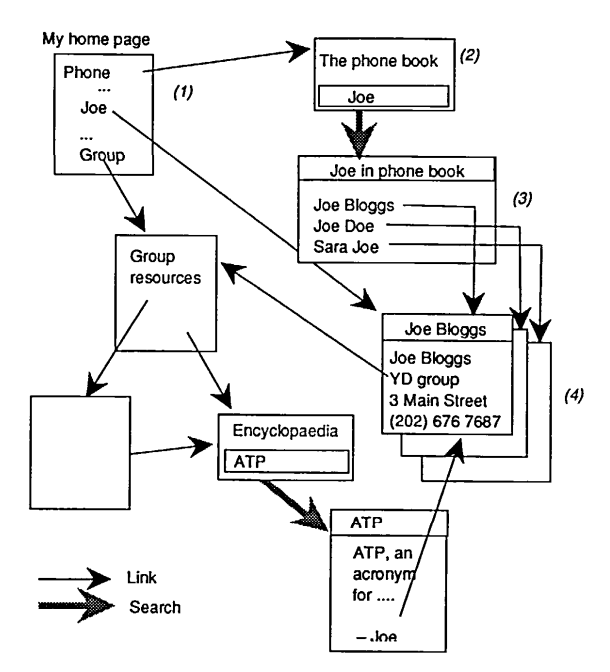
\includegraphics[keepaspectratio, width=7cm]{gambar/w3_model}
	\caption{Gambar sebuah web yang terdiri atas kumpulan \textit{link} dan indeks \citep{bernersLee1992}}
	\label{gambar:w3_model}
\end{figure}

WWW merupakan proyek Tim Berner-lee bersama teman-temannya, yang ditunjukan pada publik pada tahun 1991. WWW didesain untuk membawa sebuah semesta informasi global menggunakan teknologi yang ada. Dengan adanya WWW manusia dapat mengakses seluruh informasi melalui sebuah \textit{platform browsing} apapun. Pada masa itu, sudah ada teknologi serupa yang membuat WWW mungkin untuk dilakukan. Sistem \textit{hypertext} yang sudah ada pada saat itu, terbatas pada sistem \textit{file} lokal atau terdistribusi dan kadang hanya dikembangkan pada \textit{platform} tertentu. Selain itu, juga ada sistem pengambilan dan akses informasi seperti Alex, Gopher, Prospero, dan WAIS yang sudah mencakup area yang luas, tetapi tanpa fungsionalitas \textit{hypertext}. WWW menggabungkan teknik \textit{hypertext}, \textit{information retrieval}, dan \textit{wide area networking} \citep{bernersLee1992}.

Model yang dipakai WWW menggunakan dua paradigma dari \textit{hypertext link} dan pencarian teks yang saling melengkapi. Gambar \ref{gambar:w3_model} menunjukkan bagaimana sebuah web yang berisi informasi pribadi terbentuk pada paradigma ini. Pembaca mulai pada halaman \textit{home} (1) lalu menggunakan \textit{link} grup atau publik untuk mencari bahan informasi. Indeks seperti buku telepon (2) ditampilkan sebagai dokumen yang memungkinkan untuk melakukan input pencarian. Hasil dari pencarian berupa dokumen \textit{hypertext} virtual (3) yang menunjuk pada dokumen yang ditemukan (4) \citep{bernersLee1992}.

Terdapat fitur-fitur yang ditawarkan pada WWW yaitu:

\begin{itemize}
  \item Informasi hanya direpresentasikan sekali, sebuah rujukan (\textit{reference}) dibuat menggantikan salinan informasi.
  \item \textit{Link} memungkinkan untuk topologi informasi terus berkembang, sehingga dapat memodelkan pengetahuan manusia setiap saat tanpa kendala.
  \item Web berisi hal yang beragam mulai dari catatan kecil pada sebuah ruang kerja sampai pada basis data raksasa di benua lain.
  \item Indeks berasal dari dokumen dan dapat dicari atau melalui penelusuran \textit{link}. Sebuah indeks ditampilkan ke pengguna sebagai "halaman sampul" yang mendeskripsikan data yang diindeks dan properti dari \textit{search engine}.
  \item Dokumen pada web tidak harus memiliki bentuk fisik layaknya \textit{file}. Dokumen bisa berbentuk virtual yang dibentuk oleh server sebagai respon dari sebuah pencarian atau nama dokumen. Akibatnya dokumen dapat berbentuk \textit{views} dari basis data, atau \textit{snapshot} perubahan data.
\end{itemize}

Kebanyakan pengembangan tentang sistem \textit{hypertext} pada saat itu kebanyakan hanya berfokus pada \textit{User Interface} (UI) dan penulisan pertanyaan alih-alih pengembangan sistem yang bersifat luas (\textit{wide-area}) dan distribusi informasi dalam jangka panjang. Akibatnya, arsitektur pada sistem tersebut mengasumsikan bahwa pengguna menggunakan program aplikasi komputer yang sama pada sistem \textit{file} yang sama. Berbeda dengan WWW yang bersifat global, sehingga dihadapi dengan komputer pengguna terdistribusi dan beragam dengan tipe perangkat yang berbeda-beda. Hal ini membuat arsitektur WWW mengadopsi model klien-server. Klien bertugas memproses sebuah alamat dokumen menjadi sebuah dokumen dengan protokol jaringan tertentu. Sedangkan server menyediakan data dalam bentuk \textit{hypertext} sederhana atau dalam bentuk teks biasa, atau format data lain dengan bernegosiasi dengan klien \citep{bernersLee1992}.

Tantangan dari arsitektur tersebut adalah harus mengembangkan sebuah \textit{hypertext browser}, lebih sulit daripada mengembangkan tampilan \textit{front-end} pada sistem informasi tertentu. Walaupun demikian, memisahkan program klien dan server dengan "\textit{information bus}" akan terbayar ketika semakin banyak klien dan server bermunculan dan pembacaan universal tercapai. Menulis kode untuk sebuah server untuk data secara umum lebih sederhana karena tidak membutuhkan UI \citep{bernersLee1992}. 

\begin{figure}[H]
	\centering
	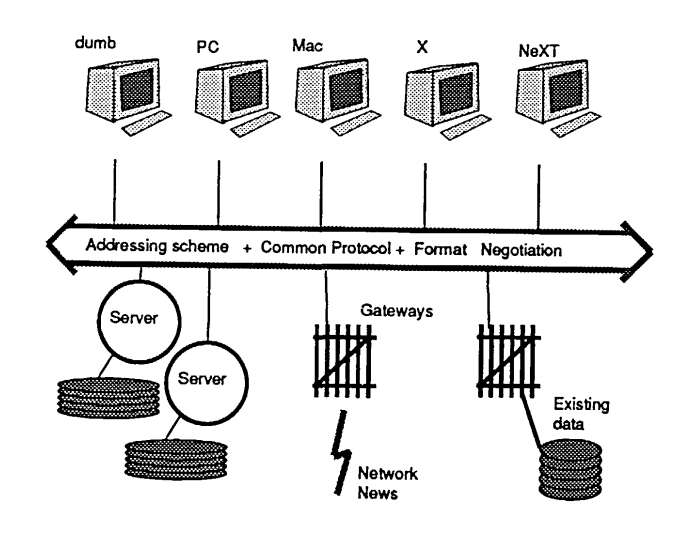
\includegraphics[keepaspectratio, width=7cm]{gambar/w3_architecture}
	\caption{Gambar arsitektur WWW \textit{link} dan indeks \citep{bernersLee1992}}
	\label{gambar:w3_architecture}
\end{figure}

Terdapat beberapa protokol yang dipakai WWW, \textit{File Transfer Protocol} (FTP), \textit{Network New Transfer Protocol} (NNTP), akses ke sistem \textit{file} terpasang (\textit{mounted}). Sebuah protokol baru yang bersifat cari dan dapatkan (\textit{search and retrieve} yang disebut HTTP, juga dianggap penting dan digunakan WWW. Lebih cepat dari FTP untuk menarik dokumen, HTTP juga memungkinkan untuk pencarian indeks. HTTP mirip dengan implementasi protokol internet yang disebutkan sebelumnya dan mirip dengan fungsionalitas protokol WAIS.

Saat ini WWW terbukti sukses dalam mewujudkan cita-citanya dalam memudahkan akses informasi global ke pengguna. Terdapat lebih dari 1 miliar situs web yang terindeks WWW \citep{huss2022} dan angka tersebut akan terus bertambah. Selain itu juga, terdapat miliaran pengguna internet yang secara otomatis juga merasakan manfaat WWW ketika melakukan pencarian di \textit{browser}. Belum lagi menyebutkan teknologi turunan yang muncul karena WWW, seperti \textit{web development}, \textit{search engine}, \textit{web API}, dan masih banyak lagi.

\section{\textit{Search Engine}}

\textit{Search engine} adalah program perangkat lunak yang memungkinkan untuk mencari kumpulan situs web berdasarkan kata kunci yang dimasukkan oleh pengguna. \textit{Search engine} lalu mencocokkan kata pencarian dengan basis data yang dimiliki. \textit{Search engine} adalah contoh sistem pengambilan informasi berskala masif \citep{seymour2011}.

Sejarah dimulai pengembangan \textit{search engine} dimulai pada tahun 1990. Alat pertama yang digunakan untuk mencari di internet adalah Archie. Archie dibuat pada 1990 oleh Alan Emtage, seorang mahasiswa di universitas McGill di Montreal. Basis data Archie terdiri atas direktori \textit{file} dari ratusan sistem. Ketika pengguna mencari di basis data Archie dalam bentuk nama \textit{file}, Archie dapat memberi tahu lokasi dari salinan \textit{file} tersebut. Archie tidak mengindeks konten dari \textit{file} tersebut. Pada periode tertentu, Archie mengunjungi situs - situs FTP terbuka yang diketahui, membuat daftar \textit{file} tersebut, dan membuat indeks yang dapat dicari. Perintah-perintah yang digunakan untuk Archie adalah perintah UNIX, sehingga untuk bisa menggunakan Archie, pengguna harus memiliki pengetahuan tentang UNIX \citep{seymour2011}.

Pada tahun 1994, seorang mahasiswa \textit{Computer Science Engineer} Universitas Washington, membuat WebCrawler pada waktu senggangnya. Awalnya WebCrawler merupakan aplikasi Desktop, bukan layanan web seperti saat ini. WebCrawler hidup di atas web dengan basis data berisi halaman dari 4000 situs web berbeda. WebCrawler merupakan \textit{search engine} web pertama yang menyediakan fitur pencarian teks secara penuh. WebCrawler berhasil dibuat pada 20 April 1994 oleh Brian Pinkerton dan dibeli America Online pada 1 Juni 1995, lalu dijual lagi ke Excite pada 1 April 1997. Yang membedakan WebCrawler dengan pendahulunya adalah penggunaan robot web pertama yang mampu mengindeks setiap kata pada halaman web, menyimpan URL, dan sebuah judul maksimal 100 kata \citep{seymour2011}.

AltaVista, dibuat pada tahun 1995, pernah menjadi \textit{search engine} yang paling populer sebelum naiknya Google. \textit{Crawler} yang dipakai AltaVista dibuat oleh Louis Moner, dan yang membuat pengindeks adalah Michael Burrows. AltaVista merupakan \textit{search engine} tercepat pada masanya yang dapat menangani jutaan \textit{hit} tiap harinya tanpa adanya penurunan performa. Satu hal yang sangat membedakan AltaVista dengan \textit{search engine} lain pada masa itu adalah mampu memproses bahasa natural sebagai kata masukan untuk mencari web. Pengguna dapat menulis kalimat atau pertanyaan untuk mendapatkan respon pintar. Sebagai contoh, pengguna dapat menulis “Dimana London ?” tanpa mendapatkan jutaan hasil pencarian yang tidak diinginkan karena mengandung “di” atau “mana” \citep{seymour2011}.

\begin{figure}[H]
	\centering
	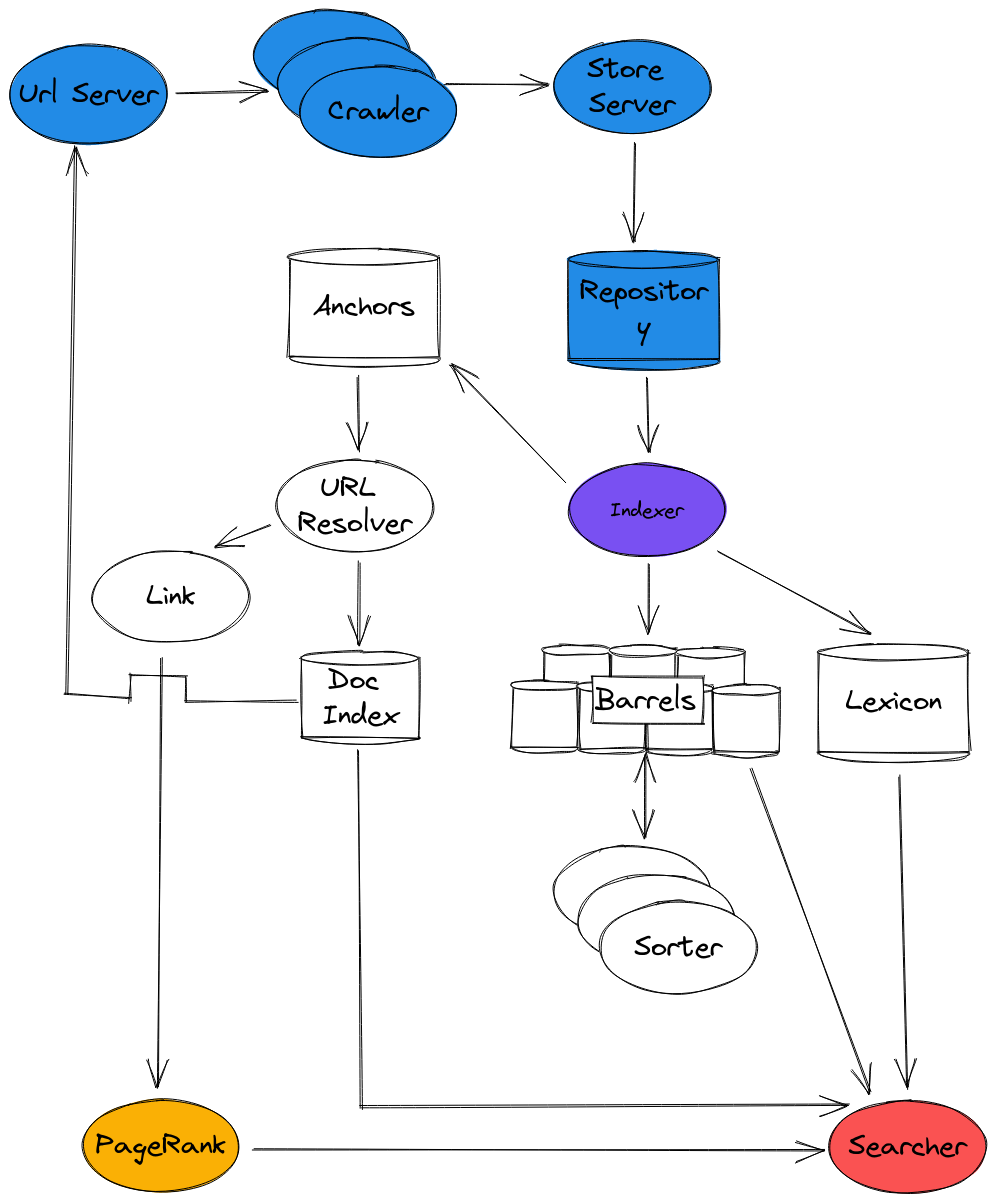
\includegraphics[keepaspectratio, width=\textwidth]{gambar/google_architecture_filled}
	\caption{\emph{High Level Google Architecture} \citep{brin1998anatomy}}
	\label{gambar:google_architecture_filled}
\end{figure}

Google dibuat pada tahun 1998, oleh Lawrence Page dan Sergey Brin. Pada saat itu, metode utama untuk menelusuri WWW adalah dengan menggunakan \textit{search engine} atau melalui situs kumpulan indeks berkualitas tinggi yang disusun oleh manusia, yang pada saat itu, yang paling populer adalah Yahoo!. Kedua metode tersebut memiliki permasalahan. Yahoo! walaupun mampu menyajikan topik - topik populer tetapi bersifat sangat subjektif, memiliki biaya yang mahal karena membutuhkan tenaga manusia, dan tidak bisa mencakup topik-topik yang bersifat esoterik \citep{brin1998anatomy}. Sedangkan untuk \textit{search engine} otomatis yang berlandaskan pada pencocokkan kata kunci biasanya menampilkan halaman web berkualitas rendah. Untuk memperburuk keadaan, pengiklan berusaha menarik perhatian pengguna dengan memanfaatkan kelemahan \textit{search engine}. Google dibuat dengan harapan untuk menjawab masalah - masalah tersebut.

Google diharapkan dapat menjadi \textit{search engine} yang \textit{scalable}, karena halaman web yang terus bertumbuh pesat. Dibutuhkan teknologi \textit{crawling} yang cepat untuk bisa mengumpulkan dokumen web dan memperbaharuinya. Perangkat penyimpanan harus digunakan seefisien mungkin untuk menyimpan indeks, dan jika memungkinkan, menyimpan dokumen web itu sendiri. Sistem pengindeksan harus bisa memproses ratusan \textit{Giga Byte} data secara efisien. Pemrosesan kueri harus ditangani secepat mungkin pada tingkat ratusan atau ribuan kueri per-detik. Hal ini juga didukung dengan semakin cepat, besar, dan murahnya perangkat keras komputer dari waktu ke waktu.

Selain \textit{scalable}, Google juga diharapkan menghasilkan hasil pencarian yang lebih berkualitas. Pada saat Google dikembangkan, hasil pencarian \textit{search engine} dipenuhi dengan hasil "sampah" karena hanya mengandalkan indeks tanpa menilai apakah halaman web yang ditampilkan memenuhi keinginan pengguna. Pengguna tidak dapat mengecek satu-per-satu dari ratusan sampai ribuan hasil pencarian yang ditampilkan. Algoritma Pagerank dikembangkan untuk Google digunakan untuk merangking seberapa penting halaman web berdasarkan struktur \textit{link} graf WWW.

Sampai saat ini, \textit{search engine} baru terus bermunculan. Pada 2004, Yahoo! yang sebelumnya terkenal sebagai direktori web, alih-alih sebagai \textit{search engine} otomatis, meluncurkan \textit{search engine} sendiri dengan menggabungkan fitur-fitur beberapa \textit{search engine} yang mereka akuisisi. Dilanjutkan pada tahun 2005 MSN Search, dan pada tahun 2009 Bing oleh Microsoft \citep{seymour2011}. Walaupun demikian, Google tetap mendominasi pasar \textit{search engine} hingga saat ini (lihat gambar \ref{gambar:search_engine_market_share}).

\begin{figure}[H]
	\centering
	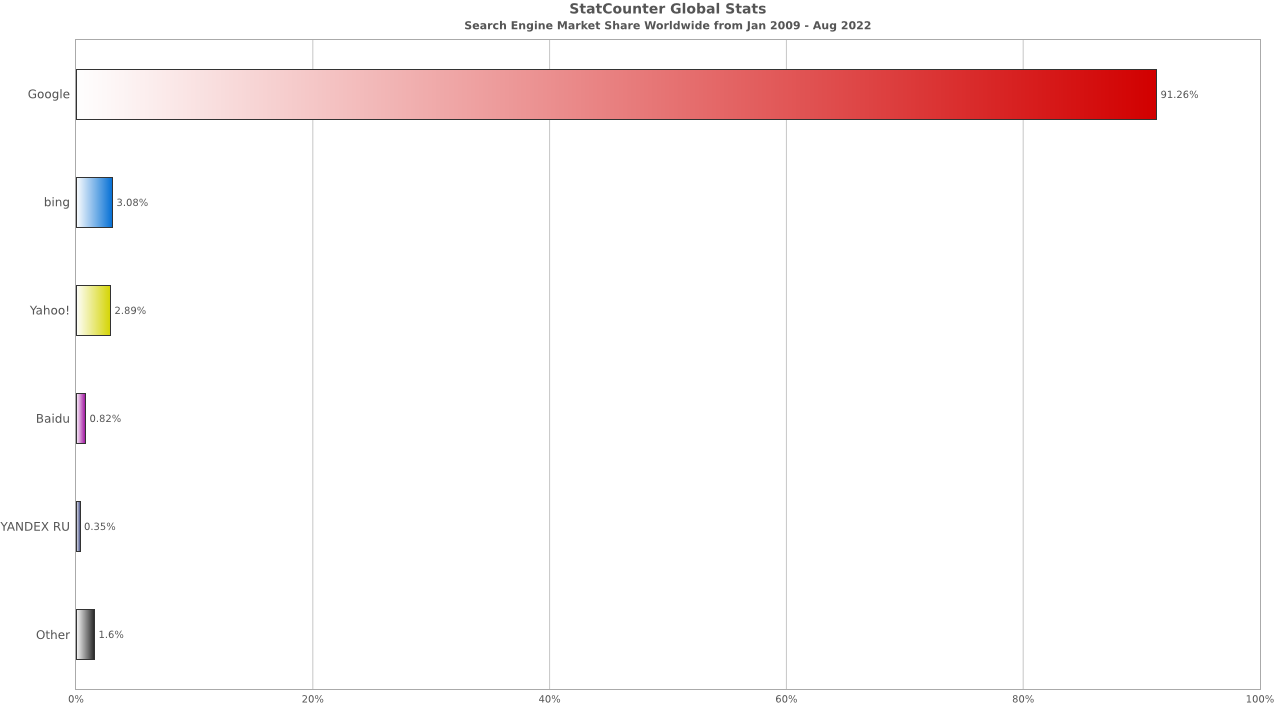
\includegraphics[keepaspectratio, width=14cm]{gambar/search_engine_market_share}
	\caption{Pangsa pasar \textit{search engine} \citep{gsc2022marketshare}}
	\label{gambar:search_engine_market_share}
\end{figure}

\section{Teori Graf}

\begin{figure}[!htb]
\begin{minipage}{0.48\textwidth}
	\centering
	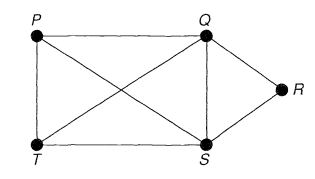
\includegraphics[width=.7\linewidth]{gambar/graph_example}
	\caption{Contoh graf \citep{wilson1996}}
	\label{gambar:graph_example}
\end{minipage}\hfill
\begin{minipage}{0.48\textwidth}
	\centering
	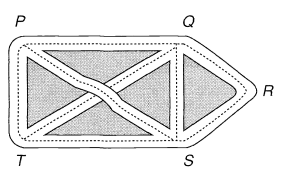
\includegraphics[width=.7\linewidth]{gambar/graph_example_2}
	\caption{Contoh peta jalan yang dapat diandaikan sebagai graf \citep{wilson1996}}
	\label{gambar:graph_example_2}
\end{minipage}
\end{figure}

\begin{figure}[H]
	\centering
	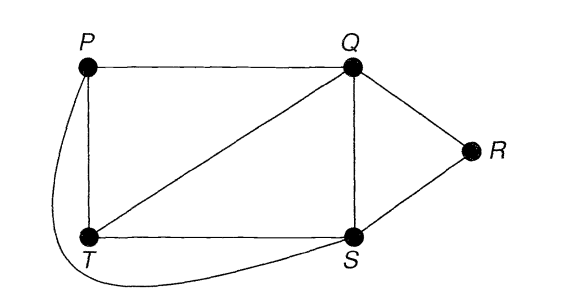
\includegraphics[keepaspectratio, width=0.48\textwidth]{gambar/graph_example_3}
	\caption{}
	\label{gambar:graph_example_3}
\end{figure}

Graf adalah sebuah representasi dari himpunan titik (\textit{node / vertice}) dan bagaimana titik-titik tersebut saling terhubung tanpa memperdulikan sifat metriknya \citep{wilson1996}. Pada gambar \ref{gambar:graph_example} merupakan contoh graf, dengan $P$, $Q$, $R$, $S$, $T$ merupakan titik, dan masing-masing terhubung dengan garis (\textit{edge}). Garis yang menghubungkan titik $P$ dan $S$ disebut dengan $PS$, sedangkan garis yang menghubungkan titik $Q$ dan $T$ disebut dengan $QT$. Persilangan antara $PS$ dan $QT$ tidak disebut sebagai titik, karena keduanya tidak saling bersilangan, melainkan saling melompati layaknya gambar \ref{gambar:graph_example_2}. Selanjutnya, kedua graf dianggap sama, jika dan hanya jika titik yang berkorespondensi sama-sama terhubung dengan garis yang sama dengan garis pada graf lainnya \citep{wilson1996}. Sebagai contoh, graf pada gambar \ref{gambar:graph_example_3} merupakan graf yang sama dengan graf pada gambar \ref{gambar:graph_example} \citep{wilson1996}. 


\begin{figure}[!htb]
\begin{minipage}{0.48\textwidth}
	\centering
	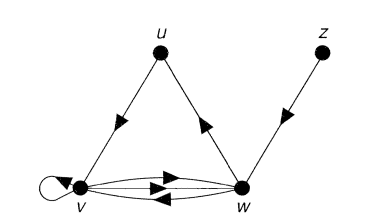
\includegraphics[width=.7\linewidth]{gambar/digraph_example}
	\caption{Contoh digraf \citep{wilson1996}}
	\label{gambar:digraph_example}
\end{minipage}\hfill
\begin{minipage}{0.48\textwidth}
	\centering
	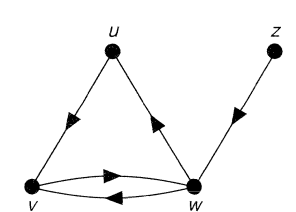
\includegraphics[width=.7\linewidth]{gambar/simple_digraph_example}
	\caption{Contoh digraf sederhana \citep{wilson1996}}
	\label{gambar:simple_digraph_example}
\end{minipage}
\end{figure}

Garis pada graf dapat diberikan arah. Garis pada graf yang berarah disebut sebagai busur (\textit{arc}). Graf yang memiliki arah pada garisnya disebut dengan graf berarah (\textit{directed graph / digraph} / digraf) yang terdiri atas himpunan titik dan busur \citep{wilson1996}. Pada digraf di gambar \ref{gambar:digraph_example} terdapat himpunan titik $u$, $v$, $w$, dan $z$, dengan busur $uv$, $vv$, $vw (2\times)$, $wv$, $wu$, dan $zw$. Sebuah digraf disebut sebagai digraf sederhana jika himpunan busurnya tidak ada yang sama (\textit{distinct}) dan tidak memiliki \textit{loop} (contoh: busur $vv$) \citep{wilson1996}. Digraf pada gambar \ref{gambar:simple_digraph_example} adalah contoh digraf sederhana.

\section{Pagerank}

World Wide Web memberikan tantangan baru dalam hal memperoleh informasi karena besar dan beragam isi-nya. Terdapat miliaran halaman web saat ini. Halaman web tersebut sangat beragam mulai dari "Apa yang Joe makan hari ini ?" sampai ke jurnal tentang \textit{information retrieval}. Belum lagi tantangan lain \textit{search engine} harus menghadapi pengguna yang kurang berpengalaman dan banyaknya halaman web yang sudah dibuat sedemikian rupa untuk memanipulasi fungsi perangkingan yang dipakai \textit{search engine}.

Walaupun demikian, tidak seperti dokumen biasa, halaman web berisi \textit{hypertext} dan menyediakan banyak informasi tambahan pada setiap teks yang ada pada halaman web, seperti struktur \textit{link} dan \textit{link} teks. Pagerank memanfaatkan keuntungan struktur \textit{link} pada web untuk menghasilkan sebuah \textit{ranking} seberapa penting pada setiap halaman web secara global. \textit{Ranking} ini membantu \textit{search engine} dan pengguna untuk menelusuri luas dan beragamnya World Wide Web.

Jika World Wide Web diibaratkan pada sebuah graf berarah, halaman web adalah titik graf, \textit{link} adalah garis. Lalu \textit{link} yang menunjuk keluar dari titik disebut \textit{forward link}, sedangkan \textit{link} yang menunjuk kedalam titik disebut \textit{backlink} (Lihat gambar \ref{gambar:web_graph_ilustration}). Sangat sulit untuk mengetahui semua \textit{backlink} suatu halaman web, tetapi sangat mudah untuk mengetahui semua \textit{forward link} suatu halaman web yaitu dengan cara mengunduh halaman web tersebut \citep{ilprints422}. Setiap halaman web memiliki jumlah \textit{backlink} yang beragam. Pada saat Pagerank diteliti, halaman \textit{home} NetScape memiliki 62.804 \textit{backlink} dibandingkan halaman web kebanyakan yang hanya memiliki beberapa \textit{backlink}. Secara umum suatu halaman web jika memiliki banyak \textit{backlink} dapat dianggap lebih penting daripada halaman web lain yang memiliki lebih sedikit \textit{backlink}. Perhitungan jumlah sitasi sederhana pernah digunakan untuk memprediksi pemenang Nobel masa depan \citep{ilprints422}. 

\begin{figure}[H]
	\centering
	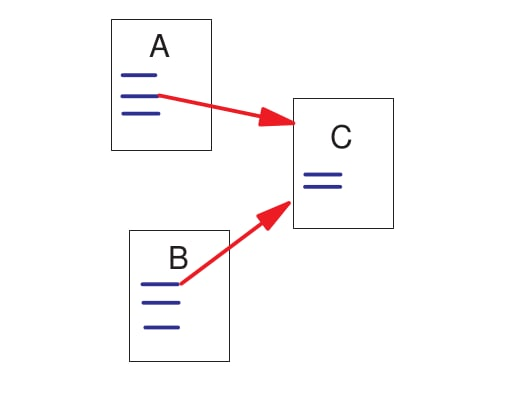
\includegraphics[keepaspectratio, width=7cm]{gambar/web_graph_ilustration}
	\caption{A dan B adalah \textit{backlink} dari C \citep{ilprints422}}
	\label{gambar:web_graph_ilustration}
\end{figure}

Yang membuat Pagerank menarik adalah sekedar menghitung jumlah sitasi atau \textit{backlink} saja tidak cukup untuk membuat \textit{ranking} halaman web sesuai dengan apa yang pengguna anggap sebagai penting. Sebagai contoh, jika ada suatu halaman web yang memiliki \textit{backlink} dari situs terkenal, misal halaman \textit{home} Yahoo.com, mungkin itu hanya satu \textit{link} tetapi berasal dari halaman yang penting. Halaman tersebut seharusnya memiliki \textit{ranking} di atas halaman web yang memiliki banyak \textit{backlink} tetapi berasal dari tempat yang tidak jelas. Pagerank berusaha untuk mewujudkan perangkingan yang selaras dengan makna penting di mata pengguna hanya dengan menggunakan struktur \textit{link} \citep{ilprints422}.

Pagerank dapat didefinisikan pada persamaan \ref{eq:1}. Halaman web merupakan $u$. Himpunan $F_u$ adalah kumpulan halaman $u$ yang menunjuk halaman lain atau disebut dengan \textit{forward link} dan $B_u$ adalah himpunan halaman yang menunjuk ke $u$ atau disebut dengan \textit{backlink}. $C_u = |F_u|$ adalah jumlah \textit{link} dari $u$, sedangkan $c$ adalah faktor yang digunakan untuk normalisasi (sehingga jumlah total \textit{ranking} semua halaman web adalah konstan) dan $c < 1$. $E(u)$ adalah vektor yang berkorespondensi dengan \textit{ranking} halaman web. $||\pi'||_1 = 1$. Iterasi perhitungan terus dilakukan sampai konvergen. Jika diubah kedalam persamaan matriks, maka persamaan \ref{eq:1} dapat diubah menjadi persamaan \ref{eq:2}. Dimana $X$ adalah matriks persegi yang baris dan kolomnya berkorespondensi dengan halaman web, dengan elemen $X_{u,v} = \frac{1}{C_v}$ jika terdapat \textit{link} pada halaman $v$ ke halaman $u$ atau $X_{u,v} = 0$ jika tidak ada.

Berdasarkan persamaan \ref{eq:2}, Algoritma Pagerank secara sederhana dapat didefinisikan pada algoritma \ref{alg:1}. Vektor ranking awal-awal dapat didefinisikan sebagai vektor apapun yang berkorespondensi dengan halaman web (misal $E$). 

\begin{breakablealgorithm}
\label{alg:1}
\floatname{algorithm}{Algoritma}
\caption{Algoritma Pagerank \citep{ilprints422}}
\begin{algorithmic}[1]
  \State $\pi_0 \gets \text{vektor ranking awal-awal (misal $E$)}$
  \Do
    \State $\pi_{i+1} \gets X\pi_i$
    \State $\delta \gets ||\pi_i||_1 - ||\pi_{i+1}||_1$
    \State $\pi_{i+1} \gets \pi_{i+1} + \delta E$
  \doWhile{$||\pi_{i+1} - \pi_i||_1 > \epsilon$}
\end{algorithmic}
\end{breakablealgorithm}

\section{\textit{Distributed Pagerank Computation} (DPC)}

Telah dijelaskan sebelumnya, masalah dari algoritma Pagerank biasa adalah besarnya memori utama yang dibutuhkan untuk bisa menyimpan matriks $X$ (lihat persamaan \ref{eq:2}). Oleh karena itu, dirumuskan algoritma Pagerank terdistribusi. DPC, dirumuskan oleh \citet{zhuetal2005distributedPagerank}, memakai mekanisme interaksi sederhana antara \textit{cluster} dan lalu lintas komunikasi rendah. Ditinjau dari perspektif matematika, dibuktikan bahwa algoritma DPC setara dengan metode \textit{Iterative Aggregation-Disaggregation} (IAD) dengan \textit{Block Jacobi smoothing}. DPC juga memiliki keunggulan dibandingkan dengan algoritma Pagerank biasa yaitu, matriks-matriks dipecah menjadi matriks agregasi dan matriks lokal sehingga ukurannya cukup kecil untuk disimpan di memori utama, sehingga mempercepat komputasi karena tiap iterasi memerlukan sedikit operasi I/O pada \textit{disk}. Selanjutnya, Vektor Pagerank lokal konvergen lebih cepat pada beberapa \textit{cluster} tertentu, berbeda dengan Pagerank biasa karena terdapat komputasi tidak perlu pada \textit{cluster} yang sudah konvergen \citep{zhuetal2005distributedPagerank}.

\subsection{Algoritma Pagerank versi DPC}

Secara esensi algoritma Pagerank pada artikel asli \citet{ilprints422}, dan algoritma Pagerank yang dipakai pada algoritma DPC pada artikel \citet{zhuetal2005distributedPagerank} adalah sama. Hanya terdapat beberapa penyesuaian. Pertama vektor $E$, merupakan probabilitas \textit{random walker} melompat ke halaman web lain secara acak, diganti dengan $(1 - d)$. $d$ disebut sebagai \textit{damping factor} merupakan probabilitas \textit{random walker} mengikuti \textit{link} yang tersedia. Nilai $d$ pada penelitian \citet{zhuetal2005distributedPagerank} adalah $0.85$. Yang kedua, jika vektor $E$ pada algoritma Pagerank di artikel \citet{ilprints422} digunakan pada langkah tersendiri, sedangkan nilai $d$ pada artikel \citet{zhuetal2005distributedPagerank} dipakai langsung dalam menentukan nilai elemen pada matriks transisi.

\begin{equation}
	\label{eq:5-1}
	P_{ij}= 
	\begin{cases}
		\frac{d}{C_j} + \frac{(1-d)}{N} & j \to i \\
		\frac{(1-d)}{N} & j \not\to i \text{ dan } C_j \not=0 \\
		\frac{1}{N} & C_j = 0
	\end{cases}
\end{equation}

Matriks transisi pada algoritma DPC didefinisikan sebagai matriks $P$. Matriks $P$ didefinisikan pada persamaan \ref{eq:5-1}. $C_j$ adalah jumlah \textit{forward link} dari halaman $j$. $j \to i$ adalah halaman $j$ memiliki \textit{link} menuju halaman $i$.

Selanjutnya algoritma Pagerank yang dipakai DPC didefinisikan pada algoritma \ref{alg:1.1}

\begin{breakablealgorithm}
	\label{alg:1.1}
	\floatname{algorithm}{Algoritma}
	\caption{Algoritma Pagerank yang dipakai DPC \citep{zhuetal2005distributedPagerank}}
	\begin{algorithmic}[1]
		\State Definisikan $\pi^0$ awal-awal
		\State $k \gets 0$
		\State \label{alg:1.1.step:start_loop} $\pi^{\sim k+1} \gets P \pi^k$
		\State $\pi^{k+1} \gets \frac{\pi^{\sim k+1}}{||\pi^{\sim k+1}||_1}$
		\State Jika $||\pi^{k+1} - \pi^k|| < \epsilon$  berhenti dan kembalikan nilai $\pi^{k+1}$
		\State $k \gets k+1$
		\State Ulangi langkah \ref{alg:1.1.step:start_loop}
	\end{algorithmic}
\end{breakablealgorithm}

\subsection{Algoritma IAD}

Jika \textit{link} pada kumpulan web dibuat kedalam graf, maka graf tersebut akan memiliki sebuah struktur menyerupai blok, karena mayoritas dari \textit{link} tersebut bersifat \textit{intra-host}, merujuk halaman yang masih di dalam \textit{host} yang sama. Oleh karena itu, jika dilakukan perjalanan acak pada kumpulan web tersebut dapat dilihat sebagai rantai Markov \textit{Nearly Completely Decomposable} (NCD) \citep{zhuetal2005distributedPagerank}. Rantai Markov NCD adalah rantai Markov yang dapat dipartisi sehingga peluang dari keadaan awal ke keadaan selanjutnya lebih sering menunjuk keadaan yang berada di dalam partisinya dibandingkan di luar partisinya \citep{kontovasilisMitrou1995}. Sebelum dijelaskan tentang DPC, akan dijelaskan metode IAD terlebih dahulu.

Misal G adalah himpunan bilangan bulat $\{1,...,N\}$. Misal $G_1,...G_n, n \leq N$ adalah grup agregasi dari elemen-elemen di $G$. Himpunan-himpunan $G_i, i = 1,...,n$, adalah saling lepas dan $\cup^n_{i=1}G_i=G$. Misal $N_i$ adalah ordo dari himpunan $G_i$, atau jumlah elemen-elemen di $G_i$ \citep{zhuetal2005distributedPagerank}. 

Misal $R$ adalah matriks agregasi $n \times N$, yang memenuhi persamaan \ref{eq:3} \citep{zhuetal2005distributedPagerank}.

\begin{equation}
	\label{eq:3}
	R_{ij}= 
	\begin{cases}
			1 & j \in G_i\\
			0 & \text{lainnya}
	\end{cases}
\end{equation}

Dilakukan partisi pada vektor positif $\pi$ menjadi $(\pi^T_1,\pi^T_2,...,\pi^T_n)^T$ berdasarkan $\{G_i\}$. $\pi_i$ adalah subvektor dengan dimensi $N_i$ \citep{zhuetal2005distributedPagerank}.

Maka dapat didefinisikan matriks disagregasi $S(\pi)$ $N \times n$ sebagai persamaan \ref{eq:4} \citep{zhuetal2005distributedPagerank}.
\begin{equation}
	\label{eq:4}
	S(\pi) = 
	\begin{pmatrix}
		S(\pi)_1 & 0 & \ldots & 0 \\
		0 & S(\pi)_2 & \ldots & 0 \\
		\vdots & \vdots & \ddots & \vdots \\
		0 & 0 & \ldots & S(\pi)_n
	\end{pmatrix}
\end{equation}
Dimana $S(\pi)_i$ adalah sebuah kolom vektor yang mewakili \textit{censored stationary distribution} dari halaman-halaman di \textit{cluster} $G_i$. Ingat bahwa $RS(\pi) = I$ \citep{zhuetal2005distributedPagerank}.

\begin{breakablealgorithm}
	\label{alg:2}
	\floatname{algorithm}{Algoritma}
	\caption{Algoritma IAD \citep{zhuetal2005distributedPagerank}}
	\begin{algorithmic}[1]
		\State $||\pi^0|| \gets 1$
		\State $\pi^0 \gets$ Pilih bilangan bulat positif
		\State $k \gets 0$
		\Do
			\State Buat matriks agregasi $RPS(\pi^k)$ dan selesaikan persamaan linear \ref{eq:5}. Dimana $||z|| = 1$
			\begin{equation}
				\label{eq:5}
				RPS(\pi^k)z^k = z^k
			\end{equation}
			\State $\pi^{\sim k+1} \gets TS(\pi^k)z^k$
			\State $\pi^{k+1} \gets \frac{\pi^{\sim k+1}}{||\pi^{\sim k+1}||_1}$
			\State $k \gets k + 1$
		\doWhile{$||\pi^{k+1} - \pi^k|| < \epsilon$}
	\end{algorithmic}
\end{breakablealgorithm}

Misal $T = M^{-1}N$ adalah sebuah matriks berasal dari operasi pemisahan matriks dari $I - P = M - N$. Dimana $M$ adalah matriks non-singular (bisa dilakukan invers) dan operasi pemisahan matriksnya adalah \textit{weak regular}, yang berarti $M^{-1} \geq 0$ dan $M^{-1}N \geq 0$ \citep{mishra2016}. Untuk menyelesaikan persamaan linear $(I - P)\pi = 0$, maka dapat dirumuskan algoritma Iteration Aggregation Disaggregation (IAD) yang dapat dilihat pada algoritma \ref{alg:2} \citep{zhuetal2005distributedPagerank}.

\subsection{Algoritma DPC}

Sebelum langsung membahas algoritma DPC, akan didefinisikan beberapa notasi terlebih dahulu. $e=(1,...,1)^T$. Matriks transisi $P$ dipartisi menjadi beberapa blok berdasarkan $\{G_i\}$ menjadi seperti persamaan \ref{eq:6} \citep{zhuetal2005distributedPagerank}.
\begin{equation}
\label{eq:6}
	P =
	\begin{pmatrix}
		P_{11} & P_{12} & \ldots & P_{1n} \\
		P_{21} & P_{22} & \ldots & P_{2n} \\
		\vdots & \vdots & \ddots & \vdots \\
		P_{n1} & P_{n2} & \ldots & P_{nn}
	\end{pmatrix}
\end{equation}
Dilambangkan blok baris ke-$i$ sebagai persamaan \ref{eq:7}
\begin{equation}
\label{eq:7}
	P_{i*} \overset{\Delta}{=} (P_{i1},\ldots,P_{in})
\end{equation}
dan dilambangkan blok kolom ke-$i$ sebagai persamaan \ref{eq:8}
\begin{equation}
\label{eq:8}
	P_{*i} \overset{\Delta}{=}
	\begin{pmatrix}
		P_{1i} \\
		\vdots \\
		P_{ni} 
	\end{pmatrix}
\end{equation} 

Setiap blok diagonal $P_{ii}$ adalah matriks persegi dan merupakan matriks \textit{intra-cluster} \textit{link} dari \textit{cluster} $G_i$, sementara blok-blok di luar diagonal merupakan struktur \textit{link} antar-\textit{cluster}. Selanjutnya, matriks agregat $A = RPS(\pi)$ adalah matriks transisi antar \textit{cluster}. Maka dapat dibuat algoritma DPC pada algoritma \ref{alg:3} \citep{zhuetal2005distributedPagerank}.

\begin{breakablealgorithm}
\label{alg:3}
\floatname{algorithm}{Algoritma}
\caption{Algoritma DPC \citep{zhuetal2005distributedPagerank}}
\begin{algorithmic}[1]
  \State Buat matriks transisi lokal untuk tiap \textit{cluster} $G_i$ berdasarkan $P$ 
		\begin{equation} \label{alg:3.step:trivial:1} Q_i = LocalTransitionMatrix(G_i) \forall G_i \in G \end{equation}
  \State 
		\begin{equation} \label{alg:3.step:trivial:2} \pi_i^0 = Pagerank(Q_i, \frac{e}{N_i}, \epsilon) \forall G_i \in G \end{equation}
		Ket: $e = [1, 1, ..., 1]^T; N_i \rightarrow \text{jumlah anggota $G_i$}$
  \State Inisialisasi $k = 0$
	\State
		\begin{equation} \label{alg:3.step:2:1} A^k = RPS(\pi^k) \end{equation}
		Ket: $R \rightarrow \text{persamaan \ref{eq:3}}; P \rightarrow \text{persamaan \ref{eq:5-1}}; S(\pi) \rightarrow \text{persamaan \ref{eq:4}}$
	\State
		\begin{equation} \label{alg:3.step:2:2} z^k = Pagerank(A^k, \frac{e}{n}, \epsilon) \end{equation}
		Ket: $n \rightarrow \text{banyaknya anggota }G$
	\State \label{alg:3.step:3:1} $\forall G_i \in G$ buat sebuah \textit{extended local transition matrix} $(N_i + 1) \times (N_i + 1)$. Dimana skalar $\alpha^k$ membuat jumlah nilai kolom dari $B^k_i$ adalah satu
		\begin{equation}
			\label{eq:9}
			B_i^k =
			\begin{pmatrix}
				P_{ii} 		& \frac{(P_{i*}S(\pi^k)z^k - P_{ii}\pi_i^kz_i)}{(1 - z^k_i)} \\
				e^TP_{*i} & \alpha^k
			\end{pmatrix}
		\end{equation}
	\State \label{alg:3.step:3:2} Hitung vektor \textit{extended local Pagerank}. Dimana $\beta^{k+1}_i$ adalah skalar
		\begin{equation}
			\begin{pmatrix}
				\omega^{k+1}_i \\
				\beta^{k+1}_i
			\end{pmatrix}
			= Pagerank(B^k_i, \frac{e}{(N_i + 1)}, \epsilon)
		\end{equation}
	\State \label{alg:3.step:3:3} \begin{equation} \pi^{\sim k+1}_i = \frac{1 - z^k_i}{\beta^{k+1}_i} \omega^{k+1}_i \end{equation}
	\State \label{alg:3.step:normalization} \begin{equation} \pi^{k+1} = \frac{\pi^{\sim k+1}}{||\pi^{\sim k+1}||_1} \end{equation}
	\State $k = k+1$
	\State Jika persamaan \ref{alg:3.eq:1} terpenuhi, berhenti dan berikan $\pi^{k}$ sebagai hasil akhir. Jika sebaliknya, kembali ke langkah \ref{alg:3.step:2:1}
		\begin{equation} \label{alg:3.eq:1} ||\pi^{k+1} - \pi^k|| < \epsilon \end{equation}
\end{algorithmic}
\end{breakablealgorithm}

\subsection{Contoh Nilai dari tiap simbol algoritma DPC}

Akan diberikan contoh nilai dari tiap simbol algoritma DPC yang sudah dijelaskan sebelumnya. Misal diberikan graf berarah halaman web pada gambar \ref{gambar:web_graph}. Jika dibuat matriks $P$, berdasarkan persamaan \ref{eq:5-1}, dan jika $d = 0,85$, maka matriks P yang terbentuk akan menjadi seperti matriks \ref{eq:p_matrix_example}. Nilai dari elemen $P_{1,1}$ diperoleh dari perhitungan $\frac{1 - d}{N} = \frac{1 - 0,85}{7} = 0,02143$, karena antara halaman 1 ("unj.ac.id") tidak memiliki \textit{forward link} ke dirinya sendiri. Nilai dari elemen $P_{2,1}$ diperoleh dari perhitungan  $\frac{d}{C_j} + \frac{1 - d}{N} = \frac{0,85}{5} + \frac{1 - 0,85}{7} = 0,23393$ karena antara halaman 1 memiliki \textit{forward link} ke halaman 2 ("unj.ac.id/sejarah-unj"). Nilai elemen $P_{1,2}$ sampai elemen $P_{7,2}$ diperoleh dari perhitungan $\frac{1}{N} = \frac{1}{7} = 0,14286$, karena halaman 2 tidak memiliki \textit{forward link} ke halaman manapun.

\begin{figure}[H]
	\centering
	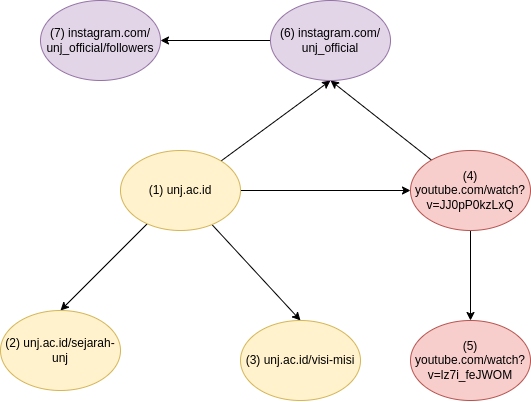
\includegraphics[height=7cm, keepaspectratio]{gambar/web_graph}
	\caption{}
	\label{gambar:web_graph}
\end{figure}

\begingroup
\makeatletter
\def\f@size{10}
\check@mathfonts
\begin{equation}
\label{eq:p_matrix_example}
	P =
	\begin{pmatrix}
		0,02143 & 0,14286 & 0,14286 & 0,02143 & 0,14286 & 0,02143 & 0,14286 \\
		0,23393 & 0,14286 & 0,14286 & 0,02143 & 0,14286 & 0,02143 & 0,14286 \\
		0,23393 & 0,14286 & 0,14286 & 0,02143 & 0,14286 & 0,02143 & 0,14286 \\
		0,23393 & 0,14286 & 0,14286 & 0,02143 & 0,14286 & 0,02143 & 0,14286 \\
		0,02143 & 0,14286 & 0,14286 & 0,44643 & 0,14286 & 0,02143 & 0,14286 \\
		0,23393 & 0,14286 & 0,14286 & 0,44642 & 0,14286 & 0,02143 & 0,14286 \\
		0,02143 & 0,14286 & 0,14286 & 0,02143 & 0,14286 & 0,87143 & 0,14286 \\
	\end{pmatrix}
\end{equation}
\endgroup

Dari matriks P sebelumnya, maka dapat dipecah layaknya pada persamaan \ref{eq:6}, menjadi matriks \ref{eq:separated_p_matrix_example}.

\begin{equation}
\label{eq:separated_p_matrix_symbol}
	P =
	\begin{pmatrix}
		P_{1,1} & P_{1,2} & P_{1,3} \\
		P_{2,1} & P_{2,2} & P_{2,3} \\
		P_{3,1} & P_{3,2} & P_{3,3} \\
	\end{pmatrix}
\end{equation}

\begingroup
\makeatletter
\def\f@size{8}
\check@mathfonts
\begin{equation}
\label{eq:separated_p_matrix_example}
	P =
	\begin{pmatrix}
		\begin{pmatrix}
			0,02143 & 0,14286 & 0,14286 \\
			0,23393 & 0,14286 & 0,14286 \\
			0,23393 & 0,14286 & 0,14286 \\
		\end{pmatrix} &
		\begin{pmatrix}
			0,02143 & 0,14286 \\
			0,02143 & 0,14286 \\
			0,02143 & 0,14286 \\
		\end{pmatrix} &
		\begin{pmatrix}
			0,02143 & 0,14286 \\
			0,02143 & 0,14286 \\
			0,02143 & 0,14286 \\
		\end{pmatrix} \\ \\

		\begin{pmatrix}
			0,23393 & 0,14286 & 0,14286 \\
			0,02143 & 0,14286 & 0,14286 \\
		\end{pmatrix} &
		\begin{pmatrix}
			0,02143 & 0,14286 \\
			0,44643 & 0,14286 \\
		\end{pmatrix} &
		\begin{pmatrix}
			0,02143 & 0,14286 \\
			0,02143 & 0,14286 \\
		\end{pmatrix} \\ \\

		\begin{pmatrix}
			0,23393 & 0,14286 & 0,14286 \\
			0,02143 & 0,14286 & 0,14286 \\
		\end{pmatrix} &
		\begin{pmatrix}
			0,44642 & 0,14286 \\
			0,02143 & 0,14286 \\
		\end{pmatrix} &
		\begin{pmatrix}
			0,02143 & 0,14286 \\
			0,87143 & 0,14286\\
		\end{pmatrix} \\
	\end{pmatrix}
\end{equation}
\endgroup

Dari matriks $P_{1,1}$, $P_{2,2}$, dan $P_{3,3}$ dapat diperoleh matriks transisi lokal $Q_1$, $Q_2$, dan $Q_3$ yang tiap kolomnya dinormalisasi yang dapat dilihat pada matriks \ref{eq:q_i_example}.

\begingroup
\makeatletter
\def\f@size{10}
\check@mathfonts
\begin{align}
\label{eq:q_i_example}
	Q_1 =
	\begin{pmatrix}
		0,0438 & 0,33333 & 0,33333 \\
		0,4781 & 0,33333 & 0,33333 \\
		0,4781 & 0,33333 & 0,33333 \\
	\end{pmatrix} &
	Q_2 =
	\begin{pmatrix}
		0,0458 & 0,5 \\
		0,9542 & 0,5 \\
	\end{pmatrix} &
	Q_3 =
	\begin{pmatrix}
		0,024 & 0,5 \\
		0,976 & 0,5 \\
	\end{pmatrix}
\end{align}
\endgroup

Selanjutnya dari graf di gambar \ref{gambar:web_graph} dapat ditemukan 3 domain, yaitu domain 1 adalah "unj.ac.id" dengan anggota halaman "unj.ac.id", "unj.ac.id/sejarah-unj", dan "unj.ac.id/visi-misi" yang dapat dinotasikan sebagai $G_1 = \{1, 2, 3\}$. Domain 2 adalah "youtube.com" dengan anggota halaman "youtube.com/watch?v=JJ0pP0kzLxQ" dan "youtube.com/watch?v=lz7i$\_$feJWOM" yang dapat dinotasikan sebagai $G_2 = \{4, 5\}$. Yang terakhir domain 3 "instagram.com" dengan anggota halaman "instagram.com/unj$\_$official" dan "instagram.com/unj$\_$official/followers" $G_3 = \{6, 7\}$. Jika dibuat matriks R maka dapat dilihat pada matriks \ref{eq:r_matrix_example}. Elemen $R_{1,1}$ sampai elemen $R_{1,3}$ mendapat nilai 1 karena halaman 1 sampai 3 merupakan anggota $G_1$, sedangkan elemen $R_{1,4}$ sampai elemen $R_{1,7}$ mendapat nilai 0 karena halaman 4 sampai 7 bukan anggota $G_1$.

\begin{equation}
\label{eq:r_matrix_example}
	R =
	\begin{pmatrix}
		1 & 1 & 1 & 0 & 0 & 0 & 0 \\
		0 & 0 & 0 & 1 & 1 & 0 & 0 \\
		0 & 0 & 0 & 0 & 0 & 1 & 1 \\
	\end{pmatrix}
\end{equation}

Pada setiap halaman web tersebut, pada tiap anggota domain-nya dapat dijalankan algoritma Pagerank. Setelah konvergen, keluaran dari algoritma Pagerank pada tiap domainnya adalah beberapa vektor $S(\pi)_1 = \{0,25974; 0,37013;  0,37013\}$, $S(\pi)_2 = \{0,35088; 0,64912\}$, dan $S(\pi)_3 = \{0,35088; 0,64912\}$. Jika dibuat matriks $S(\pi)$ maka akan terbentuk matriks \ref{eq:s_phi_matrix_example}.

\begingroup
\makeatletter
\def\f@size{10}
\check@mathfonts
\begin{equation}
\label{eq:s_phi_matrix_example}
	S(\pi) =
	\begin{pmatrix}
		0,25974 & 0 & 0 \\
		0,37013 & 0 & 0 \\
		0,37013 & 0 & 0 \\
		0 & 0,35088 & 0 \\
		0 & 0,64912 & 0 \\
		0 & 0 & 0,35088 \\
		0 & 0 & 0,64912 \\
	\end{pmatrix}
\end{equation}
\endgroup

Setelah diperoleh matriks $R$, $P$, $S(\pi)$ maka dapat diperoleh matriks $A$, dengan mengalikan ketiga matriks tersebut, sehingga memperoleh matriks \ref{eq:a_matrix_example}.

\begin{equation}
\label{eq:a_matrix_example}
	A =
	\begin{pmatrix}
		0,44434882 & 0,30075792 & 0,30075792 \\
		0,27783429 & 0,34962928 & 0,20050528 \\
		0,27783429 & 0,34962577 & 0,49875328 \\
	\end{pmatrix}
\end{equation}

Selanjutnya diperoleh vektor $z$ dengan melakukan perhitungan Pagerank sampai konvergen dengan memasukan matriks $A$ sebagai matriks transisi, dan vektor $\frac{e}{n} = [\frac{1}{3}, \frac{1}{3}, \frac{1}{3}]^T$ sebagai vektor \textit{ranking} awal-awal. Hasil dari vektor $z$ dapat dilihat pada vektor \ref{eq:z_vector_example}.      

\begin{equation}
\label{eq:z_vector_example}
	z =
	\begin{pmatrix}
		0,35118 \\ 
		0,26756 \\ 
		0,38127 \\
	\end{pmatrix}
\end{equation}

Dari vektor dan matriks sebelumnya dapat dibentuk matriks $B_i$. Karena terdapat 3 domain, maka matriks $B_i$ yang terbetuk adalah matriks $B_1$, $B_2$, dan $B_3$. Proses pembentukan matriks $B_1$ dapat dilihat pada persamaan \ref{eq:b_1_example}.

\begin{align}
\label{eq:b_1_example}
	B_1 & = & 
	\begin{pmatrix}
		P_{1,1} & \frac{P_{1,\ast} \times S(\pi) \times z - P_{1,1} \times \pi_1 \times z_1}{1 - z_1} \\
		e^T \times P_{\ast,1} & \alpha
	\end{pmatrix} \nonumber \\
	%%%%%
	& = &
	\begin{pmatrix}
		\begin{pmatrix}
			0,02143 & 0,14286 & 0,14286 \\
			0,23393 & 0,14286 & 0,14286 \\
			0,23393 & 0,14286 & 0,14286 \\
		\end{pmatrix} & 
		\begin{pmatrix}
			0,10025 \\ 
			0,10025 \\ 
			0,10025 \\
		\end{pmatrix} \\\\
		\begin{pmatrix}
			1,00001 & 1,00002 & 1,00002
		\end{pmatrix} & 
		\begin{pmatrix}
			0,69924
		\end{pmatrix}
	\end{pmatrix} \\ \nonumber
	%%%%%%%
	& = &
	\begin{pmatrix}
		0,02143 & 0,14286 & 0,14286 & 0,10025 \\
		0,23393 & 0,14286 & 0,14286 & 0,10025 \\
		0,23393 & 0,14286 & 0,14286 & 0,10025 \\
		1,00001 & 1,00002 & 1,00002 & 0,69924 \\
	\end{pmatrix} \\ \nonumber
\end{align}

Dari \textit{extended local matrix} $B_1$ dapat diperoleh \textit{local pagerank vector} untuk domain 1. Vektor yang diperoleh dapat dilihat pada vektor \ref{eq:extended_local_pagerank_vector_example}. Di mana elemen baris 1 sampai baris 3 merupakan nilai vektor $\omega_1$, sedangkan baris 4 merupakan nilai $\beta_1$.

\begin{equation}
\label{eq:extended_local_pagerank_vector_example}
	\begin{pmatrix}
		\omega_1 \\
		\beta_1
	\end{pmatrix}
	=
	\begin{pmatrix}
		0,09005 \\
		0,10689 \\
		0,10689 \\
		0,69617
	\end{pmatrix}
\end{equation}

\subsection{Analisis Konvergen}

Dibuktikan konvergensi metode \textit{Block Jacobi} pada skenario Pagerank. Pertama-tama diberikan sebuah lema yang diambil dari penelitian \citet{courtoisSemal1986} \citep{zhuetal2005distributedPagerank}:

\textbf{Lema 1}. Iterasi
\begin{equation}
	\label{eq:11}
	\pi^{k+1} = \frac{T\pi^k}{||T\pi^k||_1}
\end{equation}  
akan konvergen ketika kondisi-kondisi berikut terpenuhi:
\begin{itemize}
	\item $\rho(T) = 1$
	\item $T$ \textit{irreducible}
	\item $T$ asiklik
\end{itemize}

$\rho(T)$ adalah \textit{spectral radius} dari matriks $T$ atau merupakan nilai mutlak terbesar dari himpunan \textit{eigenvalue} matriks $T$. Nilai \textit{eigenvalue} dari matriks $T$ dapat diperoleh dengan cara menghitung determinan dari $T - \lambda I$. Dimana $\lambda$ adalah vektor atau himpunan \textit{eigenvalue}.

\citet{neumannPlemmons1978} membuktikan bahwa iterasi matriks yang diturunkan dari \textit{weak regular splitting} matriks $I - P$ akan memenuhi syarat pertama dan kedua dari Lema 1 jika matriks $P$ stokastik dan \textit{irreducible}.

Misal $D$ adalah blok diagonal dari $I - P$. Misal $L$ adalah blok bagian segitiga bawah dari $P$, dan $U$ adalah blok bagian segitiga atas dari $P$. Berdasarkan dari operasi pemisahan matriks $I - P = D - (L + U)$, iterasi matriks dari metode \textit{Block Jacobi} adalah persamaan \ref{eq:12}

\begin{equation}
	\label{eq:12}
	T = D^{-1}(L+U)
\end{equation}

Karena $(I - P_{ii})^{-1} \geq 0$ dan $(L + U) \geq 0$, maka operasi pemisahan di atas adalah \textit{weak regular}. Karena $P$ adalah stokastik dan \textit{irreducible}, maka $T$ memenuhi syarat pertama dan kedua Lema 1.

Namun, sifat asiklik dari $P$ tidak cukup untuk menjadi sifat asiklik dari $T$. Untungnya skenario Pagerank juga terdapat lema lain:

\textbf{Lema 2}. Jika $P > 0$ adalah matriks transisi dari sebuah rantai markov dan dipartisi berdasarkan persamaan \ref{eq:6}. Misal $T$ adalah matriks iterasi yang didefinisikan pada persamaan \ref{eq:12}, atau disebut dengan matriks \textit{Block Jacobi}. $T$ adalah asiklik jika dan hanya jika $n > 2$.

Semua syarat pada Lema 1 terpenuhi ketika $n > 2$. Akibatnya dapat dirumuskan teorema:

\textbf{Teorema 1}. Jika $P > 0$ adalah matriks transisi dari rantai Markov dan dipartisi berdasarkan persamaan \ref{eq:6}. Misal T adalah matriks iterasi yang didefinisikan pada persamaan \ref{eq:12}, atau disebut dengan matriks \textit{Block Jacobi}. Jika $n > 2$, maka persamaan \ref{eq:11} akan selalu konvergen tepat pada titik $\hat{x}$ dari $P\hat{x} = \hat{x}$. 

Penjelasan lebih lengkap dari analisis konvergen dapat dibaca pada penelitian \citet{zhuetal2005distributedPagerank}.

\subsection{\textit{Communication Overhead}}

Karena DPC bersifat distributif, maka dibutuhkan komunikasi bagi setiap \textit{cluster} untuk menyatukan \textit{ranking} halaman web. Dianalisa \textit{communication overhead} atau ongkos memori saat komunikasi dari algoritma DPC. Pesan yang dikirim berupa vektor dan tidak ada matriks yang dikirim. Vektor $v$ dikirim kedalam bentuk kumpulan data berbentuk \textit{pair} yang berisi index $i$ dan nilai $v_i$ > 0. Index adalah kombinasi dari ID \textit{cluster} dan sebuah nilai \textit{hash} dari string URL. $Pos(.)$ melambangkan jumlah elemen positif pada sebuah vektor atau matriks. Sehingga ukuran dari pesan sebanding dengan nilai $Pos(v)$. Matriks \textit{sparse} (matriks yang mengandung banyak nilai 0) $\bar{P}$ dipakai dibandingkan matriks $P$. Misal $\bar{L}$ dan $\bar{U}$ adalah blok yang terletak di segitiga bawah dan atas pada matriks $\bar{P}$ secara terpisah. Matriks $\bar{P}$ dapat didefinisikan sebagai berikut:

\begin{equation}
	\bar{P_{ij}} =
	\begin{cases}
		\frac{d}{C_j} & j \rightarrow i \\
		0 & \text{lainnya}
	\end{cases}
\end{equation}

Baris ke-\ref{alg:3.step:trivial:1} dan ke-\ref{alg:3.step:trivial:2} dari algoritma DPC membutuhkan komunikasi \textit{trivial}. Pada baris ke-\ref{alg:3.step:2:1} dan baris ke-\ref{alg:3.step:2:2} algoritma DPC, \textit{cluster} $G_i$ mengirim koordinator dalam bentuk sebuah vektor $\bar{P}_{*i}\pi_i$, yang sama dengan kolom ke-$i$ dari $\bar{P}S(\pi)$. Perlu dicatat bahwa subvektor ke-$i$ dari $\bar{P}_{*i}\pi_i$ dikirim sebagai skalar $e^T\bar{P}_{ii}\pi_i$. Nilai dari lalu lintas komunikasi sebanding dengan $Pos((\bar{L} + \bar{U})S(\pi))$ yang berarti lebih kecil dari $Pos(\bar{L} + \bar{U})$. Tabel \ref{table:2} menunjukkan perbandingan pada graf web nyata \citep{zhuetal2005distributedPagerank}.

\begin{table}[h!]
	\centering
	\caption{Perbandingan jumlah elemen positif pada graf web yang diuji \citep{zhuetal2005distributedPagerank}}
	\label{table:2} 
	\begin{tabular}{|c|c|c|}
		\hline
			Graf web & $Pos(\bar{L} + \bar{U})$ (juta) & $Pos((\bar{L} + \bar{U})S(\pi))$ (juta) \\
		\hline
		
		\hline
			ST01 & 40 & 8 \\
			ST03 & 484 & 165 \\
			CN04 & 150 & 35 \\
		\hline
	\end{tabular}
\end{table}

Pada baris ke-\ref{alg:3.step:3:1} sampai baris ke-\ref{alg:3.step:3:3}, koordinator mengirim subvektor ke-$i$ dari $\bar{P}S(\pi)z$ ke \textit{cluster} $G_i$. Jadi biaya komunikasi adalah $Pos((\bar{L} + \bar{U})S(\pi)z)$, lebih kecil dari $N$.

Pada baris ke-\ref{alg:3.step:normalization}, \textit{cluster}-\textit{cluster} lokal mengirim vektor $\widetilde{\pi}^{k+1}_i$ ke koordinator yang melakukan normalisasi. Biaya komunikasinya adalah $O(N)$.

Secara keseluruhan, seluruh \textit{communication overhead} besarnya adalah $O(Pos((\bar{L} + \bar{U})S(\pi))) + O(N)$.
%!TEX root = ./template-skripsi.tex
%-------------------------------------------------------------------------------
%                            BAB III
%               			PEMBAHASAN
%-------------------------------------------------------------------------------

\chapter{METODOLOGI PENELITIAN}

\section{Tahapan Penelitian}

Terdapat tahapan-tahapan yang harus dilalui untuk melaksanakan penelitian ini. Tahapan penelitian dapat dilihat pada diagram \ref{gambar:tahapan_penelitian}. Terdapat beberapa algoritma yang belum dijelaskan sebelumnya seperti Modified DPC (MDPC) dan Random Walker. Algoritma MDPC dirumuskan karena kekurangan dari algoritma DPC yang akan dijelaskan pada bagian selanjutnya. Sedangkan algoritma Random Walker merupakan program yang mensimulasikan pergerakan kunjungan halaman web dan merupakan basis dari algoritma Pagerank \citep{ilprints422}, sehingga sangat cocok untuk dijadikan sebagai acuan untuk melakukan verifikasi hasil.

\begin{figure}[H]
	\centering
	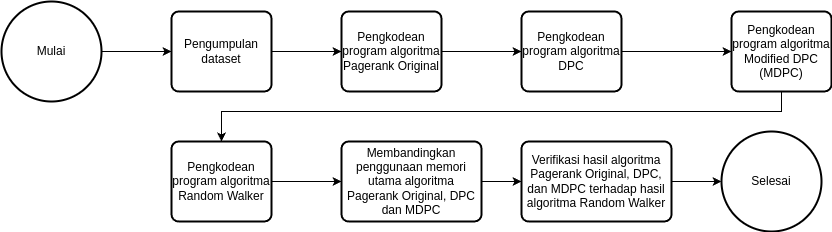
\includegraphics[keepaspectratio, width=\textwidth]{gambar/tahapan_penelitian.png}
	\caption{Diagram tahapan penelitian}
	\label{gambar:tahapan_penelitian}
\end{figure}

\section{Pengumpulan Dataset}

Penelitian ini menggunakan data yang berasal dari basis data penelitian \citet{khatulistiwa2022SearchEngine} ditambah dengan mengumpulkan data tambahan yang sama-sama diperoleh dengan menjalankan program \textit{crawling}. Data yang diperoleh disimpan ke dalam basis data MySQL dan terdapat 13 tabel atau \textit{entity} yang strukturnya dapat dilihat pada tabel-tabel berikut:
	
\begin{table}[h!]
	\centering
	\caption{Struktur tabel \textit{crawling}}
	\label{table:entity_crawling}
	\begin{tabular}{|c|c|c|}
		\hline
		\multicolumn{3}{|c|}{\textit{crawling}} \\
		\hline
		\textbf{No.} & \textbf{Atribut} & \textbf{Tipe Data} \\
		\hline
		1. & id\_crawling & int \\
		2. & start\_urls & text \\
		3. & keyword & text \\
		4. & total\_page & int \\
		5. & duration\_crawl & time \\
		6. & created\_at & timestamp \\
		\hline
	\end{tabular}
\end{table}
 
 \begin{table}[h!]
	\centering
	\caption{Struktur tabel \textit{page\_information}}
	\label{table:entity_page_information}
	\begin{tabular}{|c|c|c|}
		\hline
		\multicolumn{3}{|c|}{\textit{page\_information}} \\
		\hline
		\textbf{No.} & \textbf{Atribut} & \textbf{Tipe Data} \\
		\hline
		1. & id\_page & int \\
		2. & crawl\_id & int \\
		3. & url & text \\
		4. & html5 & tinyint \\
		5. & title & text \\
		6. & description & text \\
		7. & keywords & text \\
		8. & content\_text & text \\
		9. & hot\_url & tinyint \\
		10. & size\_bytes & bigint \\
		11. & model\_crawl & text \\
		12. & duration\_crawl & time \\
		13. & created\_at & timestamp \\
		\hline
	\end{tabular}
\end{table}

\begin{table}[h!]
	\centering
	\caption{Struktur tabel \textit{tfidf\_word}}
	\label{table:tfidf_word}
	\begin{tabular}{|c|c|c|}
		\hline
		\multicolumn{3}{|c|}{\textit{tfidf\_word}} \\
		\hline
		\textbf{No.} & \textbf{Atribut} & \textbf{Tipe Data} \\
		\hline
		1. & id\_word & int \\
		2. & word & text \\
		3. & page\_id & int \\
		4. & tfidf\_score & double \\
		\hline
	\end{tabular}
\end{table}

\begin{table}[h!]
	\centering
	\caption{Struktur tabel \textit{tfidf}}
	\label{table:entity_tfidf}
	\begin{tabular}{|c|c|c|}
		\hline
		\multicolumn{3}{|c|}{\textit{tfidf}} \\
		\hline
		\textbf{No.} & \textbf{Atribut} & \textbf{Tipe Data} \\
		\hline
		1. & id\_tfidf & int \\
		2. & keyword & text \\
		3. & page\_id & int \\
		4. & tfidf\_total & double \\
		\hline
	\end{tabular}
\end{table}

\begin{table}[h!]
	\centering
	\caption{Struktur tabel \textit{pagerank}}
	\label{table:entity_pagerank}
	\begin{tabular}{|c|c|c|}
		\hline
		\multicolumn{3}{|c|}{\textit{pagerank}} \\
		\hline
		\textbf{No.} & \textbf{Atribut} & \textbf{Tipe Data} \\
		\hline
		1. & id\_pagerank & int \\
		2. & page\_id & int \\
		3. & pagerank\_score & double \\
		\hline
	\end{tabular}
\end{table}

\begin{table}[h!]
	\centering
	\caption{Struktur tabel \textit{page\_linking}}
	\label{table:entity_page_linking}
	\begin{tabular}{|c|c|c|}
		\hline
		\multicolumn{3}{|c|}{\textit{page\_linking}} \\
		\hline
		\textbf{No.} & \textbf{Atribut} & \textbf{Tipe Data} \\
		\hline
		1. & id\_linking & int \\
		2. & page\_id & int \\
		3. & outgoing\_link & text \\
		\hline
	\end{tabular}
\end{table}

\begin{table}[h!]
	\centering
	\caption{Struktur tabel \textit{page\_tables}}
	\label{table:entity_page_tables}
	\begin{tabular}{|c|c|c|}
		\hline
		\multicolumn{3}{|c|}{\textit{page\_tables}} \\
		\hline
		\textbf{No.} & \textbf{Atribut} & \textbf{Tipe Data} \\
		\hline
		1. & id\_table & int \\
		2. & page\_id & int \\
		3. & table\_str & text \\
		\hline
	\end{tabular}
\end{table}

\begin{table}[h!]
	\centering
	\caption{Struktur tabel \textit{page\_forms}}
	\label{table:entity_page_forms}
	\begin{tabular}{|c|c|c|}
		\hline
		\multicolumn{3}{|c|}{\textit{page\_forms}} \\
		\hline
		\textbf{No.} & \textbf{Atribut} & \textbf{Tipe Data} \\
		\hline
		1. & id\_form & int \\
		2. & page\_id & int \\
		3. & form & text \\
		\hline
	\end{tabular}
\end{table}

\begin{table}[h!]
	\centering
	\caption{Struktur tabel \textit{page\_images}}
	\label{table:entity_page_images}
	\begin{tabular}{|c|c|c|}
		\hline
		\multicolumn{3}{|c|}{\textit{page\_images}} \\
		\hline
		\textbf{No.} & \textbf{Atribut} & \textbf{Tipe Data} \\
		\hline
		1. & id\_image & int \\
		2. & page\_id & int \\
		3. & image & text \\
		\hline
	\end{tabular}
\end{table}

\begin{table}[h!]
	\centering
	\caption{Struktur tabel \textit{page\_scripts}}
	\label{table:entity_page_scripts}
	\begin{tabular}{|c|c|c|}
		\hline
		\multicolumn{3}{|c|}{\textit{page\_scripts}} \\
		\hline
		\textbf{No.} & \textbf{Atribut} & \textbf{Tipe Data} \\
		\hline
		1. & id\_script & int \\
		2. & page\_id & int \\
		3. & script & text \\
		\hline
	\end{tabular}
\end{table}

\begin{table}[h!]
	\centering
	\caption{Struktur tabel \textit{page\_list}}
	\label{table:entity_page_list}
	\begin{tabular}{|c|c|c|}
		\hline
		\multicolumn{3}{|c|}{\textit{page\_list}} \\
		\hline
		\textbf{No.} & \textbf{Atribut} & \textbf{Tipe Data} \\
		\hline
		1. & id\_list & int \\
		2. & page\_id & int \\
		3. & list & text \\
		\hline
	\end{tabular}
\end{table}

\begin{table}[h!]
	\centering
	\caption{Struktur tabel \textit{page\_styles}}
	\label{table:entity_page_styles}
	\begin{tabular}{|c|c|c|}
		\hline
		\multicolumn{3}{|c|}{\textit{page\_styles}} \\
		\hline
		\textbf{No.} & \textbf{Atribut} & \textbf{Tipe Data} \\
		\hline
		1. & id\_style & int \\
		2. & page\_id & int \\
		3. & style & text \\
		\hline
	\end{tabular}
\end{table}

Dari 13 tabel tersebut, nantinya tabel yang akan dipakai adalah tabel \textit{page\_linking}, \textit{page\_information}, dan tabel \textit{pagerank}. Tabel \textit{page\_linking} memuat informasi dari halaman mana \textit{link} berasal melalui atribut \textit{page\_id} dan ke mana \textit{link} tersebut menunjuk melalui atribut \textit{url}. Untuk tabel \textit{page\_information} atribut yang dipakai hanya \textit{id\_page} dan \textit{url}. Lalu setelah perhitungan selesai, maka hasilnya akan disimpan kedalam tabel \textit{pagerank}.

Pada penelitian ini digunakan dua \textit{dataset}. \textit{Dataset} pertama yang nantinya disebut sebagai Dataset 1 merupakan \textit{dataset} gabungan dari \textit{dataset} yang diperoleh dari penelitian \citet{khatulistiwa2022SearchEngine} dan data lanjutan yang diperoleh dengan cara \textit{crawling}. Sebelumnya Dataset 1 hanya memiliki tidak lebih dari 11.000 baris halaman web \textit{page\_information} menjadi 20.493 baris dan 2.915.842 baris \textit{page\_linking}. Data \textit{page\_information} pada Dataset 1 dapat dikelompokan ke dalam 560 \textit{cluster} berdasarkan \textit{domain}-nya yang dapat dilihat pada tabel \ref{domain:dataset1}.

\begin{longtable}{|c|c|c|}
\caption{Data \textit{cluster} pada Dataset 1}
\label{domain:dataset1} \\
\hline
\textbf{No.} & \textbf{Domain} & \textbf{Jumlah Halaman} \\
\hline
1 & detik.com & 2.215 \\
2 & unj.ac.id & 2.208 \\
3 & sport.detik.com & 1.279 \\
4 & finance.detik.com & 1.098 \\
5 & repository.unj.ac.id & 1.089 \\
6 & news.detik.com & 802 \\
7 & oto.detik.com & 779 \\
8 & inet.detik.com & 671 \\
9 & support.google.com & 630 \\
10 & food.detik.com & 626 \\
\vdots & \vdots & \vdots \\
558 & codingcompetitions.withgoogle.com & 1 \\
559 & googledevelopers.blogspot.com & 1 \\
560 & skillshop.exceedlms.com & 1 \\
\hline
\end{longtable}

%filling%
Dapat dilihat pada tabel \ref{domain:dataset1}, halaman web didominasi oleh domain "detik.com" dan "unj.ac.id" beserta sub domainnya, hal ini karena saat dilakukan \textit{crawling} titik halaman web awal-awal yang di-\textit{crawl} adalah "detik.com" dan "unj.ac.id". Hal ini juga membuktikan kecendrungan dari halaman web memiliki \textit{link} yang bersifat \textit{intra-link} yaitu \textit{link} yang menunjuk halaman lain yang masih di dalam satu domain-nya, yang merupakan salah satu basis dari algoritma DPC \citep{zhuetal2005distributedPagerank}. 
%filling end%

Yang kedua, Dataset 2 merupakan \textit{dataset} kecil dan \textit{domain} kecil yang sengaja dikumpulkan untuk melihat perbedaan performa algoritma antara \textit{dataset} yang berisi banyak \textit{domain} besar dengan \textit{dataset} yang berisi \textit{domain} kecil. Batasan pada tiap \textit{domain} yang dipakai ketika mengumpulkan data adalah 20 halaman web per \textit{domain}. Pada Dataset 2 terdapat 100 baris \textit{page\_information}, 5.944 baris \textit{page\_linking}, serta 5 \textit{cluster} atau \textit{domain}. Data \textit{cluster} pada Dataset 2 dapat dilihat pada tabel \ref{domain:dataset2}.

\begin{longtable}{|c|c|c|}
\caption{Data \textit{cluster} pada Dataset 2}
\label{domain:dataset2} \\
\hline
\textbf{No.} & \textbf{Domain} & \textbf{Jumlah Halaman} \\
\hline
1 & unj.ac.id & 20 \\
2 & ppid.unj.ac.id & 20 \\
3 & fip.unj.ac.id & 20 \\
4 & fbs.unj.ac.id & 20 \\
5 & fmipa.unj.ac.id & 20 \\
\hline
\end{longtable}

\section{Kelemahan Algoritma Pagerank Original}

Algoritma Pagerank Original bekerja dengan cara melakukan iterasi perkalian antara vektor \textit{ranking} halaman web terhadap matriks transisi graf situs-situs web. Permasalahan muncul karena matriks transisi tersebut membutuhkan memori utama yang cukup besar, yaitu dengan kompleksitas $O(N^2)$. Misal jika tipe data yang dipakai adalah \textit{floating point} 64 bit dan jika pada dataset terdapat 10 ribu halaman web, maka matriks transisi yang terbentuk adalah matriks persegi 10 ribu $\times$ 10 ribu dan secara memori utama diperlukan $10.000 \times 10.000 \times 64 \text{ bit} = 6.400.000.000 \text{ bit} = 800 \text{ Mega Byte}$. Walaupun pada contoh sebelumnya cukup kecil, pada kenyataannya internet memiliki miliaran halaman web yang, jika menggunakan algoritma Pagerank Original tanpa penanganan khusus, akan memakan \textit{Peta Byte} atau bahkan \textit{Exa Byte} memori. Akibatnya jika dilakukan pada satu mesin komputer pribadi yang hanya menggunakan memori 4 \textit{Giga Byte} sampai 32 \textit{Giga Byte}, program akan \textit{crash}.

\section{Penjelasan Lanjut Algoritma DPC}

Algoritma dimulai dengan memasukan input matriks transisi $P$ dan himpunan \textit{cluster} halaman web $G$. Keduanya didapatkan dari basis data penelitian \citet{khatulistiwa2022SearchEngine}, tersusun atas dua \textit{entity} yang akan dijelaskan pada nanti pada bagian berikutnya. \textit{damping factor} $d$ yang nilainya mengikuti penelitian \citet{zhuetal2005distributedPagerank} yakni $d=0.85$, dan nilai $0 < \epsilon < 1$ untuk toleransi \textit{error}.

Selanjutnya untuk setiap \textit{cluster} $G_i$ dibuat matriks lokal transisi ukuran $N_i \times N_i$ diambil dari nilai matriks transisi $P$. Setelah itu hitung nilai Pagerank lokal $\pi^0_i$ dengan memasukan $Q_i$, nilai toleransi \textit{error} $\epsilon$, dan nilai Pagerank awal-awal adalah $\frac{e}{N_i}$. Ingat $\epsilon = [1,1,...,1]^T$ atau vektor kolom seragam yang semua nilainya satu dan $N_i$ adalah jumlah anggota $G_i$ maka $\frac{e}{N_i}$ = $[\frac{1}{N_i}, \frac{1}{N_i},...,\frac{1}{N_i}]$. Hasil dari Pagerank lokal awal tersebut adalah vektor dengan dimensi $N_i \times 1$.

Langkah selanjutnya sudah memasuki \textit{looping}. $k$ adalah jumlah iterasi. Dibuat matriks agregat $A^k = RPS(\pi^k)$. $R$ adalah matriks $n \times N$, dimana $n$ adalah panjang $G_i$ dan $N$ adalah banyaknya halaman web secara keseluruhan. $R$ didefinisikan pada persamaan \ref{eq:3}. $P$ adalah matriks transisi secara keseluruhan dengan dimensi $N \times N$. $S(\pi^k)$ matriks disagregasi $N \times n$ yang didefinisikan pada persamaan \ref{eq:4}. Matriks $A^k$ dipakai sebagai input matriks transisi untuk perhitungan Pagerank pada level kasar $z^k = Pagerank(A^k, \frac{e}{n}, \epsilon)$. Perlu diingat, karena dimensi $A^k$ adalah $n \times n$, maka dimensi vektor $\frac{e}{n}$ adalah $n \times 1$. Akibatnya dimensi vektor $z^k$ adalah $n \times 1$. Langkah ini disebut dengan solusi kasar \textit{coarse level} \citep{zhuetal2005distributedPagerank}.

Setelah itu, setiap \textit{cluster} $G_i$ buat sebuah matriks $(N_i + 1) \times (N_i + 1)$ lokal transisi yang diperbesar $B^k_i$ seperti persamaan \ref{eq:9}. Pada bagian kiri atas matriks $B^k_i$, $P_{ii}$ adalah matriks transisi lokal \textit{cluster} $G_i$. Pada bagian kiri bawah terdapat perkalian vektor baris $e^T$ dengan dimensi $1 \times N$ dan $P_{*i}$ yang merupakan matriks transisi dari halaman anggota $G_i$ ke halaman anggota $G$ dengan dimensi $N \times N_i$. Hasil akhir dari perkalian tersebut adalah sebuah vektor baris $1 \times N_i$ yang akan menempati baris terbawah dari matriks $B^k_i$ bersama dengan skalar $\alpha^k$, yang menjadi elemen paling bawah dan kanan dari matriks $B^k_i$. Nilai dari $\alpha^k$ tergantung dari jumlah total kolom paling kanan matriks $B^k_i$ yaitu sama dengan 1. Pada bagian kanan atas terdapat matriks $P_{i*}$, berdimensi $N_i \times N$ sekaligus merupakan matriks transisi dari halaman anggota $G$ ke halaman anggota $G_i$, dikalikan dengan matriks disagregasi $S(\pi^k)$ dan vektor $z^k$. Selanjutnya hasil perkalian dari ketiga matriks dan vektor tersebut dikurangi dengan perkalian matriks $P_{ii}$, vektor $\pi^k_i$, dan skalar $z_i$. Dari hasil pengurangan tersebut dibagi dengan pengurangan 1 dikurangi $z^k_i$. Hasil akhir dari operasi bagian kanan atas matriks $B^k_i$ adalah sebuah vektor kolom $N_i \times 1$ sekaligus, bersama $\alpha^k$ merupakan kolom paling kanan dari matriks $B^k_i$.

Selanjutnya hitung algoritma Pagerank dengan masukan matriks $B^k_i$ sebagai matriks transisi, vektor $\frac{e}{(N_i + 1)}$ sebagai vektor \textit{ranking} awal-awal, dan nilai $\epsilon$. Hasil akhir dari Pagerank adalah vektor kolom $N_i \times 1$. Baris pertama sampai baris ke-$N_i$ adalah vektor $\omega^{k+1}_i$ dan baris ke-$(N_i + 1)$ adalah nilai skalar $\beta^{k+1}_i$. Langkah ini disebut sebagai penghalusan (\textit{smoothing}) pada tingkat lebih halus \citep{zhuetal2005distributedPagerank}.

Setelah itu, nilai \textit{ranking} halaman pada tiap \textit{cluster} yang dilambangkan dengan $\pi^{\sim k+1}_i$ diperbaharui dengan melakukan perhitungan sesuai persamaan \ref{alg:3.step:3:3}. Selanjutnya \textit{ranking} halaman tersebut dinormalisasi sesuai persamaan \ref{alg:3.step:normalization}. Hitung selisih \textit{ranking} halaman web iterasi saat ini dengan terasi sebelumnya, jika sudah kurang dari toleransi \textit{error} $\epsilon$ maka algoritma selesai mengembalikan nilai $\pi^{k+1}$. Jika tidak, maka ulangi langkah \textit{looping}.

\section{Kelemahan Algoritma DPC}

Pada algoritma DPC, langkah untuk mendapatkan matriks $A$ memerlukan perkalian matriks $R$, matriks $P$, dan matriks $R(\pi)$. Melakukan perkalian matriks $P$ secara utuh akan menimbulkan masalah dan memakan memori utama yang cukup besar, permasalahan yang sama yang dihadapi pada Pagerank Original. Untuk mengatasi hal tersebut, diperlukan penanganan khusus saat melakukan perkalian agar bisa muat pada memori utama, dengan konsekuensi algoritma dijalankan lebih lambat karena terdapat proses memecah matriks $P$ lebih kecil, dalam penelitian ini memecah matriks $P$ menjadi beberapa vektor kolomnya ketika akan mengalikan matriks $R$ dengan $P$.

Esensi pada langkah empat sampai langkah tujuh algoritma DPC adalah mencari \textit{ranking} domain dan menyesuaikan \textit{ranking} domain tersebut dengan \textit{ranking} halaman web yang masih terisolasi pada domain-nya masing-masing. Matriks $A$ sejatinya adalah matriks transisi domain, sedangkan vektor $z$ adalah vektor \textit{ranking} dari domain. Langkah-langkah tersebut dapat disimplifikasi, pada penelitian ini dirumuskan algoritma modifikasi dari algoritma DPC yang dinamakan algoritma Modified DPC (MDPC).

\section{Algoritma Modified DPC}

Sebelumnya telah dibahas dua algoritma yaitu Pagerank Original pada penelitian \citet{ilprints422}, dan Distributed Pagerank Computation pada penelitian \citet{zhuetal2005distributedPagerank}. Diusulkan algoritma modifikasi dari algoritma DPC atau Modified DPC (MDPC). Secara garis besar MDPC hanya memangkas langkah-langkah pada algoritma DPC, berdasarkan gagasan utama DPC yaitu melakukan perhitungan terpisah \textit{ranking} halaman web berdasarkan \textit{domain}-nya, dan melakukan perhitungan penggabungan dengan menghitung \textit{ranking} \textit{domain} itu sendiri. Masalah utama dari algoritma DPC adalah langkah memperoleh matriks $A$ pada langkah \ref{alg:3.step:2:1} yang melakukan perkalian matriks $P$ secara utuh.

Definisi matriks $A$ versi MDPC yang selanjutnya akan berganti notasi menjadi $A_{mdpc}$ dapat dilihat pada persamaan \ref{eq:a_mdpc}. Makna notasi $P_{**}$ merupakan partisi matriks transisi $P$ yang sudah didefinisikan pada persamaan \ref{eq:6}, sedangkan makna dari \textit{sum} adalah nilai total dari elemen matriks.

\begin{equation}
	\label{eq:a_mdpc}
	A_{mdpc} =
	\begin{pmatrix}
		\frac{\text{sum}(P_{11})}{\text{sum}(P_{*1})} & \cdots & \frac{\text{sum}(P_{1i})}{\text{sum}(P_{*i})} \\
		\vdots & \ddots & \vdots \\
		\frac{\text{sum}(P_{i1})}{\text{sum}(P_{*1})} & \cdots & \frac{\text{sum}(P_{ii})}{\text{sum}(P_{*i})}
	\end{pmatrix}
\end{equation}

Dari web graf di gambar \ref{gambar:web_graph}, dapat dibuat contoh matriks $A_{mdpc}$. Proses perhitungan matriks $A_{mdpc}$ dapat dilihat pada persamaan \ref{eq:a_mdpc_example}.

\begingroup
\makeatletter
\def\f@size{8}
\check@mathfonts
\begin{align*}
	\text{sum}(P_{\ast,1}) = \text{sum}(
		\begin{pmatrix}
			0,02143 & 0,14286 & 0,14286 \\
			0,23393 & 0,14286 & 0,14286 \\
			0,23393 & 0,14286 & 0,14286 \\
			0,23393 & 0,14286 & 0,14286 \\
			0,02143 & 0,14286 & 0,14286 \\
			0,23393 & 0,14286 & 0,14286 \\
			0,02143 & 0,14286 & 0,14286
		\end{pmatrix}
	) = 3,00005 \\
\end{align*}

\begin{align}
	\label{eq:a_mdpc_example}
	\text{sum}(P_{\ast,2}) = \text{sum}(
		\begin{pmatrix}
			0,02143 & 0,14286 \\
			0,02143 & 0,14286 \\
			0,02143 & 0,14286 \\
			0,02143 & 0,14286 \\
			0,44643 & 0,14286 \\
			0,44642 & 0,14286 \\
			0,02143 & 0,14286
		\end{pmatrix}
	) = 2,00002 & &
	\text{sum}(P_{\ast,3}) = \text{sum}(
		\begin{pmatrix}
			0,02143 & 0,14286 \\
			0,02143 & 0,14286 \\
			0,02143 & 0,14286 \\
			0,02143 & 0,14286 \\
			0,02143 & 0,14286 \\
			0,02143 & 0,14286 \\
			0,87143 & 0,14286
		\end{pmatrix}
	) = 2,00003
\end{align}

\begin{align*}
	A_{mdpc} & = &
	\begin{pmatrix}
		\frac{\text{sum}(\begin{pmatrix}
			0,02143 & 0,14286 & 0,14286 \\
			0,23393 & 0,14286 & 0,14286 \\
			0,23393 & 0,14286 & 0,14286
		\end{pmatrix})}{3,00005} &
		\frac{\text{sum}(\begin{pmatrix}
			0,02143 & 0,14286 \\
			0,02143 & 0,14286 \\
			0,02143 & 0,14286
		\end{pmatrix})}{2,00002} &
		\frac{\text{sum}(\begin{pmatrix}
			0,02143 & 0,14286 \\
			0,02143 & 0,14286 \\
			0,02143 & 0,14286
		\end{pmatrix})}{2,00003} \\
		\frac{\text{sum}(\begin{pmatrix}
			0,23393 & 0,14286 & 0,14286 \\
			0,02143 & 0,14286 & 0,14286
		\end{pmatrix})}{3,00005} &
		\frac{\text{sum}(\begin{pmatrix}
			0,02143 & 0,14286 \\
			0,44643 & 0,14286
		\end{pmatrix})}{2,00002} &
		\frac{\text{sum}(\begin{pmatrix}
			0,02143 & 0,14286 \\
			0,02143 & 0,14286
		\end{pmatrix})}{2,00003} \\
		\frac{\text{sum}(\begin{pmatrix}
			0,23393 & 0,14286 & 0,14286 \\
			0,02143 & 0,14286 & 0,14286
		\end{pmatrix})}{3,00005} &
		\frac{\text{sum}(\begin{pmatrix}
			0,44642 & 0,14286 \\
			0,02143 & 0,14286
		\end{pmatrix})}{2,00002} &
		\frac{\text{sum}(\begin{pmatrix}
			0,02143 & 0,14286 \\
			0,87143 & 0,14286
		\end{pmatrix})}{2,00003}
	\end{pmatrix} \\
	A_{mdpc} & = &
	\begin{pmatrix}
		\frac{1,34645}{3,00005} & \frac{0,49287}{2,00002} & \frac{0,49287}{2,00003} \\
		\frac{0,8268}{3,00005} & \frac{0,75358}{2,00002} & \frac{0,32858}{2,00003} \\
		\frac{0,8268}{3,00005} & \frac{0,75357}{2,00002} & \frac{1,17858}{2,00003}
	\end{pmatrix} \\
	A_{mdpc} & = &
	\begin{pmatrix}
		0,44881 & 0,24643 & 0,24643 \\
		0,2756 & 0,37679 & 0,16429 \\
		0,2756 & 0,37678 & 0,58928
	\end{pmatrix}
\end{align*}
\endgroup

Langkah-langkah algoritma MDPC dapat dilihat pada algoritma \ref{alg:mdpc}.

\begin{breakablealgorithm}
	\label{alg:mdpc}
	\floatname{algorithm}{Algoritma}
	\caption{Algoritma MDPC}
	\begin{algorithmic}[1]
		\State Buat matriks transisi lokal $N_i \times N_i$ untuk tiap \textit{cluster} $G_i$ berdasarkan $P$ 
			\begin{equation} Q_i = LocalTransitionMatrix(G_i) \forall G_i \in G \end{equation}
			Ket:  $N_i \rightarrow \text{jumlah anggota } G_i$
		\State 
			\begin{equation} \label{alg:mdpc.step.1} \pi_i = Pagerank(Q_i, \frac{e}{N_i}, \epsilon) \forall G_i \in G \end{equation}
			Ket: $e = [1, 1, ..., 1]^T$; Dimensi $\pi_i$ adalah $N_i \times 1$ 
		\State
			\begin{equation}  z = Pagerank(A_{mdpc}, \frac{e}{n}, \epsilon) \end{equation}
			Ket: $n \rightarrow \text{banyaknya anggota }G$; Dimensi $z$ adalah $n \times 1$
		\State Perbaharui nilai $\pi_i$ dengan dikalikan nilai skalar $z_i$
			\begin{equation} \pi_i \gets \pi_i \times z_i \forall i \in 1 \ldots n \end{equation}
		\State kembalikan $\pi$ sebagai hasil akhir. $\pi$ adalah vektor gabungan $N \times 1$ dari semua $\pi_i$.
	\end{algorithmic}
\end{breakablealgorithm}

\section{Algoritma Random Walker}

Basis intiutif dari algoritma Pagerank adalah \textit{random walk} pada graf. Versi penyederhanaan dalam bentuk distribusi probabilitas \textit{random walk} pada sebuah graf web \citep{ilprints422}. Akan dibuat sebuah program yang mensimulasikan dari proses \textit{random walk} ini yang disebut Algoritma Random Walker. Algoritma Random Walker dipakai untuk membandingkan hasil perhitungan algoritma DPC, MDPC, dan Pagerank asli. Langkah-langkah pada Algoritma Random Walker dapat dilihat pada algoritma \ref{alg:random_walker}.

%filling%
Pada langkah pertama jumlah iterasi diperlukan karena pada dasarnya, berbeda dengan algoritma Pagerank yang bisa konvergen, algoritma Random Walker tidak bisa berhenti selain membatasi jumlah iterasinya. Langkah kedua mensimulasikan bahwa pengguna internet dapat berasal dari halaman web mana pun. Langkah ketiga untuk menentukan besarnya peluang \textit{walker} berpindah dari halaman web awal ke halaman lain. Matriks $P$ ini juga berisi peluang \textit{walker} melompat ke halaman web lain yang tidak memiliki \textit{link} satu sama lain atau tidak terhubung langsung.
%end filling%

\begin{breakablealgorithm}
	\label{alg:random_walker}
	\floatname{algorithm}{Algoritma}
	\caption{Algoritma Random Walker}
	\begin{algorithmic}[1]
		\State Tentukan jumlah iterasi dan jumlah $walker$ awal-awal pada setiap halaman web
		\State Instansiasi $walker$ sama banyak pada setiap halaman web
		\State Bentuk matriks $P$ sesuai persamaan \ref{eq:5-1}
		\State Untuk setiap $walker$, pindahkan $walker$ ke halaman web selanjutnya berdasarkan peluang $P_{*i}$, untuk $i$ adalah indeks halaman web $walker$ saat ini.
		\State Ulangi langkah 4 sebanyak jumlah iterasi. \textit{Ranking} halaman web ditentukan pada banyaknya jumlah $walker$ yang tinggal.
	\end{algorithmic}
\end{breakablealgorithm}

Pada penelitian ini, algoritma Random Walker tidak dipakai untuk membandingkan performa, melainkan sebatas pembanding hasil dari algoritma Pagerank, DPC, dan MDPC.

\section{Alat dan Bahan Penelitian}

Untuk melaksanakan penelitian ini digunakan perangkat keras dan lunak untuk membuat program. Perangkat keras dan perangkat lunak yang digunakan adalah sebagai berikut:

\begin{enumerate}
	\item Komputer \textit{Desktop} dengan spesifikasi CPU AMD Ryzen 5 3600, GPU RTX 2060, dan RAM 16GB
	\item Monitor Resolusi 1920x1080
	\item Koneksi internet
	\item Sistem Operasi Ubuntu 22.04
	\item Editor kode Visual Studio Code
	\item DBeaver Community Edition untuk akses basis data MySQL
	\item Bahasa pemrograman Python 3
\end{enumerate}

\section{Tahapan Pengembangan}

Akan dilakukan pengkajian efisiensi penggunaan memori utama pada algoritma Pagerank, DPC, dan MDPC. Penelitian ini merupakan sub-penelitian dari penelitian utama tentang pengembangan \textit{search engine}. Telah dilakukan penelitian sebelumnya oleh \citet{qoriiba2021perancangan} yang membuat modul \textit{crawler} dan modul pendukung lain. Selanjutnya \citet{khatulistiwa2022SearchEngine} menggabungkan modul \textit{crawler} \citet{qoriiba2021perancangan}, Google Pagerank, dan \textit{searcher} berbasis TF IDF menjadi \textit{search engine} berbasis konsol. Di saat yang berdekatan, \citet{pratama2022indexer} membuat modul \textit{indexer} menggunakan \textit{Induced Generalized Suffix Tree} dan \citet{zalghornain2022indexer} menggunakan \textit{Continuous-Bag-of-Words} dan Model \textit{Continuous Skip-Gram}. 

Karena penelitian ini merupakan sub-penelitian, maka \textit{stack} teknologi yang digunakan dalam implementasi penelitian ini akan disamakan dengan penelitian induk yaitu menggunakan bahasa pemrograman Python 3 dan basis data MySQL. Implementasi algoritma akan mengikuti algoritma-algoritma yang sudah dijelaskan sebelumnya. Perkiraan pengerjaan adalah satu bulan, dan tidak menutup kemungkinan akan memakan waktu lebih lama atau lebih cepat tergantung kesulitan dan kompleksitas yang dihadapi.

Untuk menguji penggunaan memori, waktu eksekusi, dan hasil algoritma \textit{ranking} halaman web maka dilakukan langkah-langkah berikut:
\begin{enumerate}
	\item{Dilakukan pengkodean empat program algoritma yaitu Pagerank Original, DPC, MDPC, dan Random Walker}
	\item{Ditentukan nilai masukan \textit{damping factor}, toleransi \textit{error}, serta dataset yang sama}
	\item{Jalankan program Pagerank Original, DPC, MDPC, dan Random Walker terhadap dataset 1 (20.493 Halaman)}
	\item{Bandingkan lamanya waktu, dan penggunaan memori utama algoritma Pagerank Original, DPC, dan MDPC}
	\item{Verifikasi kemiripan hasil antara algoritma Pagerank Original, DPC, dan MDPC terhadap algoritma Random Walker}
	\item{Jalankan program Pagerank Original, DPC, MDPC, dan Random Walker terhadap dataset 2 (100 Halaman)}
	\item{Bandingkan lamanya waktu, dan penggunaan memori utama algoritma Pagerank Original, DPC, dan MDPC}
	\item{Verifikasi kemiripan hasil antara algoritma Pagerank Original, DPC, dan MDPC terhadap algoritma Random Walker}
\end{enumerate}

\section{Metode Perbandingan}

Terdapat tiga hal yang dibandingkan pada penelitian ini, yang pertama adalah perbandingan penggunaan memori utama, lama waktunya algoritma dijalankan, dan kemiripan hasil yang dikeluarkan oleh ketiga algoritma. Tidak ada metode khusus untuk membandingkan penggunaan memori utama, dan lama waktu eksekusi. Ketiga algoritma hanya dijalankan lalu dapat dilihat dan dibandingkan penggunaan memori utama dan lamanya waktu eksekusi tiap algoritma. Sedangkan untuk kemiripan hasil, penelitian ini mengikuti metode yang dipakai oleh \citet{zhuetal2005distributedPagerank}, digunakan perhitungan jarak \textit{Kendall's $\tau$} atau dapat disebut sebagai $KDist$.

Rumus dari jarak $KDist$ antara vektor \textit{ranking} halaman web $\pi$ terhadap $\hat{\pi}$ secara berurutan dapat dilihat pada persamaan \ref{eq:kendall_distance}, di mana $0 \leq KDist(\pi, \hat{\pi}) \leq 1$. Semakin kecil nilai jaraknya maka dianggap lebih mirip.

\begin{equation}
	K_{ij}(\pi, \hat{\pi}) = 
	\begin{cases}
		1 & \pi_i \geq \pi_j \text{ and } \hat{\pi}_i < \hat{\pi}_j \\
		1 & \pi_i < \pi_j \text{ and } \hat{\pi}_i \geq \hat{\pi}_j \\
		0 & \text{lainnya}
	\end{cases}
\end{equation}

\begin{equation}
	\label{eq:kendall_distance}
	KDist(\pi, \hat{\pi}) = \frac{\Sigma_{1 \leq i < j \leq N} K_{ij}(\pi, \hat{\pi})}{\frac{1}{2} N(N-1)}
\end{equation}
%!TEX root = ./template-skripsi.tex
%-------------------------------------------------------------------------------
%                            	BAB IV
%               		KESIMPULAN DAN SARAN
%-------------------------------------------------------------------------------

\chapter{HASIL DAN PEMBAHASAN}

Pada bab ini akan dibagi ke dalam dua bagian yaitu pengkodean dan hasil. Pada bagian pengkodean akan dibahas implementasi algoritma ke dalam kode pemrograman. Selanjutnya pada bagian hasil akan dijelaskan hasil pengujian program terhadap data yang dipakai sehingga dapat dibuat sebuah kesimpulan pada bab selanjutnya.

\section{Pengkodean}

Akan dibahas implementasi algoritma ke dalam kode pemrograman Python. Program dapat dipisah menjadi empat bagian, yaitu tiga bagian berbeda berdasarkan algoritma yang dipakai dan bagian kode program yang dipakai bersama (\textit{shared code}). Pada bagian kode program bersama, terdapat \textit{Helper Class} yang bertugas untuk \textit{caching} dan mengakses basis data atau \textit{Helper Function} yang melakukan tugas umum seperti perhitungan matematika, mengambil alamat \textit{domain} dari \textit{string url}.

\subsection{\textit{Shared Code}}

Untuk melakukan \textit{caching}, \textit{library} Pickle dipakai. Pickle mengubah objek pada program menjadi \textit{byte stream} yang disimpan ke dalam \textit{file} berformat ".pkl". Tujuan dilakukan \textit{caching} ini untuk meringankan penggunaan memori utama dengan menyimpan objek ke \textit{disk}, dan hanya dimuat ke memori utama ketika hanya akan digunakan. Objek-objek yang disimpan ke dalam \textit{cache} adalah matriks $P$ yang dipecah berdasarkan kolomnya, matriks $Q$, matriks $P_{ii}$, matriks $P_{i*}$, matriks $P_{*i}$, dan matriks $RP$. 

Potongan kode \ref{listing:caching_class} berisi \textit{class} untuk \textit{caching} \textit{Class} Cache merupakan \textit{Parent Class} dari PCache, yang sesuai namanya, bertugas melakukan \textit{Caching} untuk matriks $P$. Selain PCache juga ada \textit{Cache Class} lain seperti, QListCache untuk matriks $Q$, PiiListCache untuk matriks $P_{ii}$, PiastListCache untuk matriks $P_{i*}$, PastiListCache untuk matriks $P_{*i}$, dan RPCache untuk matriks $RP$. Secara garis besar \textit{class} tersebut memiliki \textit{method} dan \textit{property} yang mirip, seperti nama \textit{file}, dan \textit{method} untuk menyimpan dan memuat \textit{cache}.

\begin{figure}[H]
  \centering
  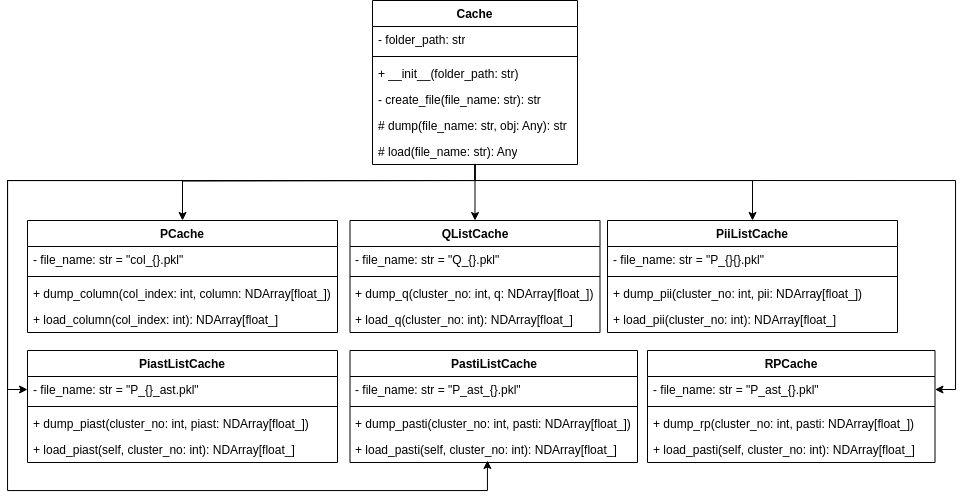
\includegraphics[keepaspectratio, width={\textwidth}]{gambar/cache_class_diagram}
  \caption{\textit{Class Diagram} dari \textit{class} Cache dan turunannya}
	\label{gambar:cache_class_diagram}
\end{figure}

Selanjutnya terdapat \textit{Class} yang bertugas menghubungkan basis data ke program. \textit{Class} DB merupakan \textit{Class} dasar untuk mengurus koneksi basis data ke program. \textit{Class} DB dibungkus ke dalam \textit{Repository Class} yang dibatasi oleh tabel tertentu dengan maksud agar tidak ada \textit{Class} yang terlalu besar karena bertanggung jawab pada banyak tugas. Sebagai contoh pada \textit{Class} PageInformationRepository bertugas mengurus tabel \textit{page\_information}. PageInformationRepository memiliki \textit{method} \textit{get\_all\_page\_informations}, sesuai namanya, mengambil semua baris dari tabel \textit{page\_information} dan dikembalikan dalam bentuk List yang berisi \textit{Class} PageInformation (lihat kode \ref{listing:db.py} dan kode \ref{listing:page_information_repository.py}). Selain PageInformationRepository, juga ada \textit{Repository Class} lain seperti PageLinkingRepository yang tugas utamanya mengambil data tabel \textit{page\_linking}, dan PagerankRepository yang tugas utamanya memasukan data hasil \textit{ranking} halaman ke tabel \textit{page\_rank\_original\_pagerank\_dpc\_paper\_version}, \textit{page\_rank\_dpc}, dan \textit{page\_rank\_modified\_dpc\_v2}.

\begin{figure}[H]
  \centering
  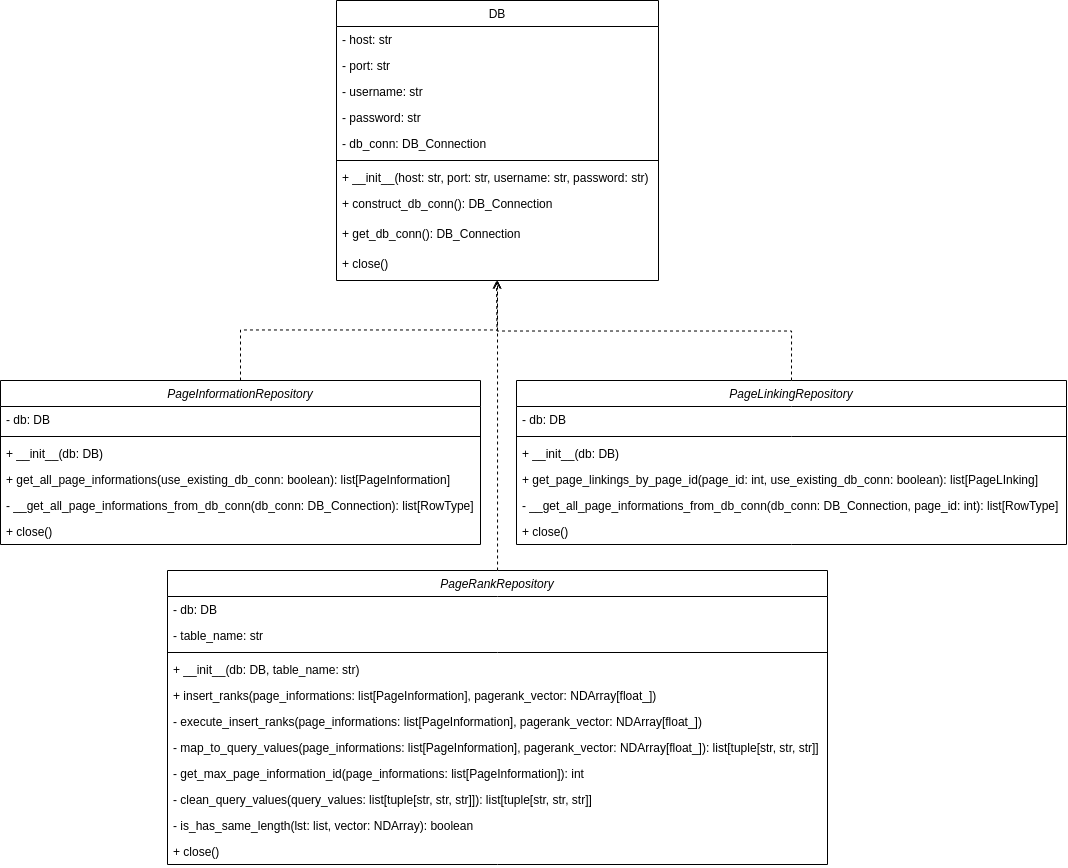
\includegraphics[keepaspectratio, width={\textwidth}]{gambar/db_class_diagram}
  \caption{\textit{Class Diagram} dari \textit{class} DB dan \textit{class} lain yang memiliki dependensi terhadapnya}
	\label{gambar:db_class_diagram}
\end{figure}

Sebelumnya sempat disinggung \textit{Class} PageInformation tanpa penjelasan lebih lanjut. \textit{Class} PageInformation merupakan salah satu dari dua \textit{Model Class} yang ada di program penelitian ini. \textit{Model Class} merupakan \textit{Class} sederhana yang memodelkan data pada program. Pada kode \ref{listing:model.py} terdapat PageInformation dan PageLinking. PageInformation menampung data baris pada tabel \textit{page\_information}. PageInformation memiliki tiga atribut yaitu \textit{index} urutan PageInformation dalam matriks, \textit{id\_page} yang diambil dari basis data, dan url yang juga diambil dari basis data. Yang kedua ada PageLinking menampung data baris pada tabel \textit{page\_linking} yang memiliki atribut \textit{outgoing\_link} yang diambil dari basis data.

Pada kode \ref{listing:helper_functions.py} terlihat \textit{helper functions} yang memiliki kegunaan tertentu yang bersifat umum. Sebagai contoh fungsi \textit{l1\_norm} mengembalikan nilai \textit{l1 norm} dari suatu List. Selanjutnya ada \textit{create\_url\_to\_page\_information\_dict} yang mengubah List yang berisi PageInformation menjadi sebuah \textit{dictionary} dengan \textit{url} sebagai kunci, dan PageInformation merupakan isinya. Fungsi \textit{sort\_page\_information\_by\_domain} mengurutkan List PageInformation berdasarkan domain-nya. Selain \textit{helper functions}, di \textit{file} yang sama, juga ada \textit{class} PageInformationClusterizer yang tugasnya adalah mengelompokan List yang berisi PageInformation berdasarkan domain-nya, hasil akhirnya adalah sebuah \textit{dictionary} yang \textit{key}-nya merupakan domain, dan \textit{value}-nya merupakan List PageInformation yang sudah dikelompokan sebelumnya.

\begin{figure}[H]
  \centering
  
\includegraphics[keepaspectratio, width={\textwidth}]{gambar/page_information_clusterizer_class_diagram}
  \caption{\textit{Class Diagram} dari \textit{class} PageInformationClusterizer}
	\label{gambar:page_information_clusterizer_class_diagram}
\end{figure}

\textit{Class} PHelper adalah sebuah \textit{class} yang bertugas untuk membuat matriks transisi $P$. \textit{Class} PHelper memiliki dependensi terhadap \textit{class} PageLinkingRepository karena untuk menentukan nilai elemennya didasari pada \textit{link} pada halaman web. Kode dan \textit{Class Diagram} PHelper secara berurutan dapat dilihat pada kode \ref{listing:PHelper.py} dan gambar \ref{gambar:p_helper_class_diagram_2}.

\begin{figure}[H]
\centering
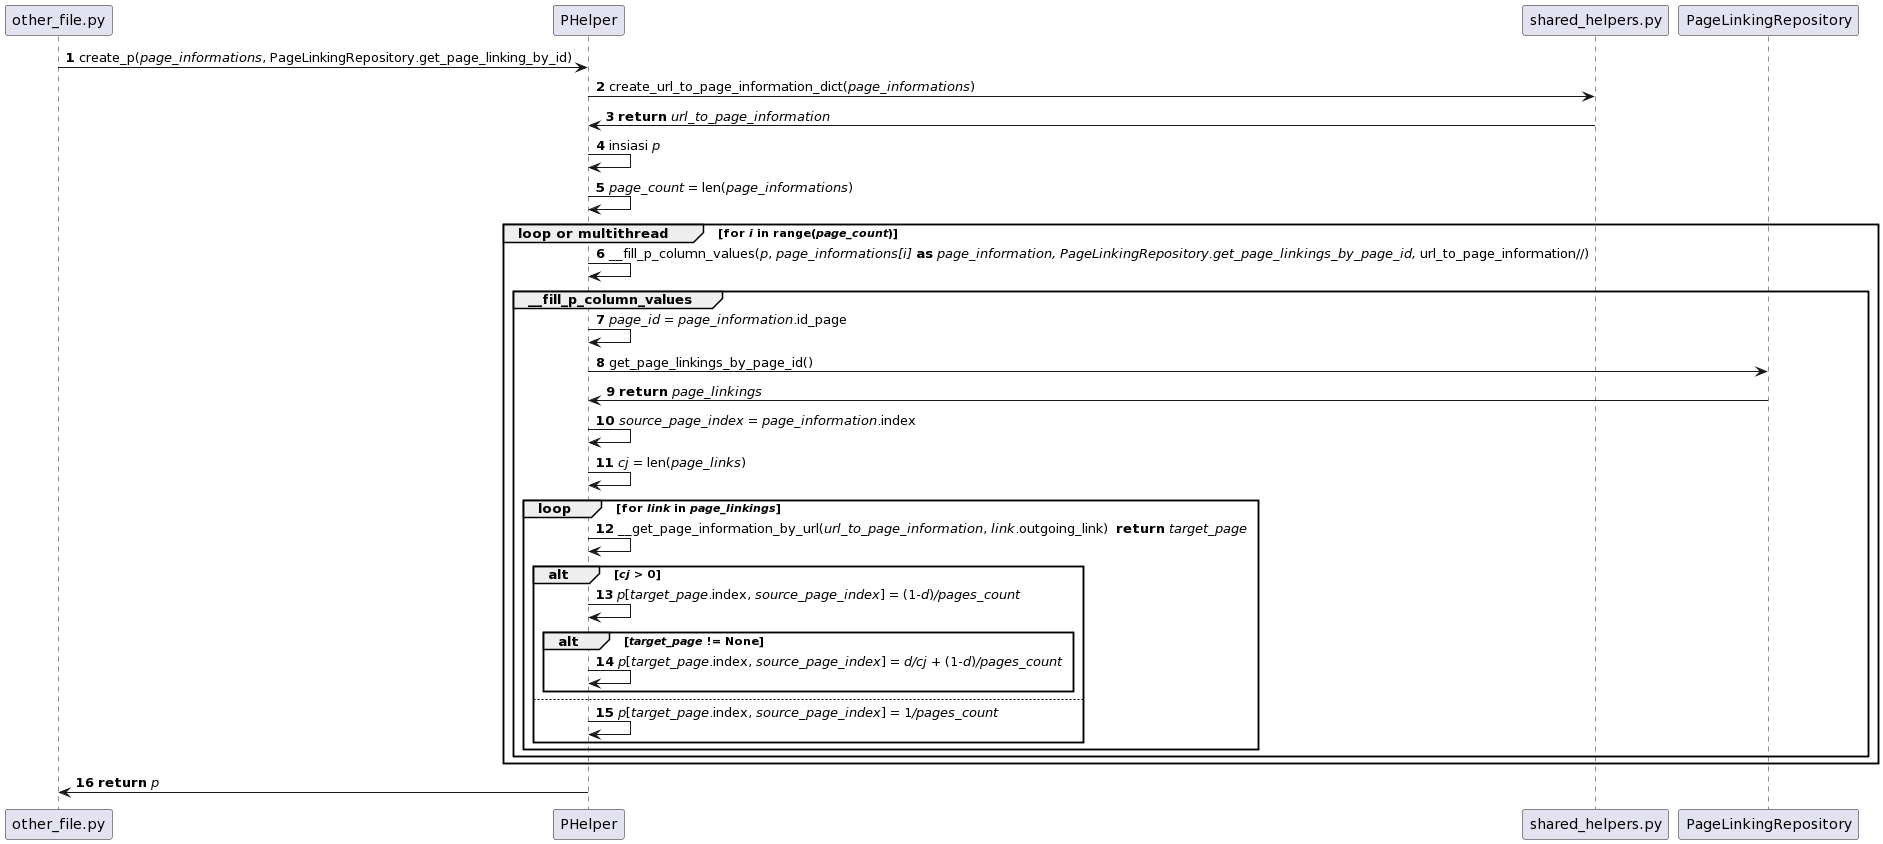
\includegraphics[width={\textheight}, height={\textwidth}, angle=270]{gambar/p_helper_sequence_diagram_2}
\caption{Diagram alir ketika membentuk matriks transisi $P$ di \textit{class} PHelper}
\label{gambar:p_helper_sequence_diagram_2}
\end{figure}

\begin{figure}[H]
\centering
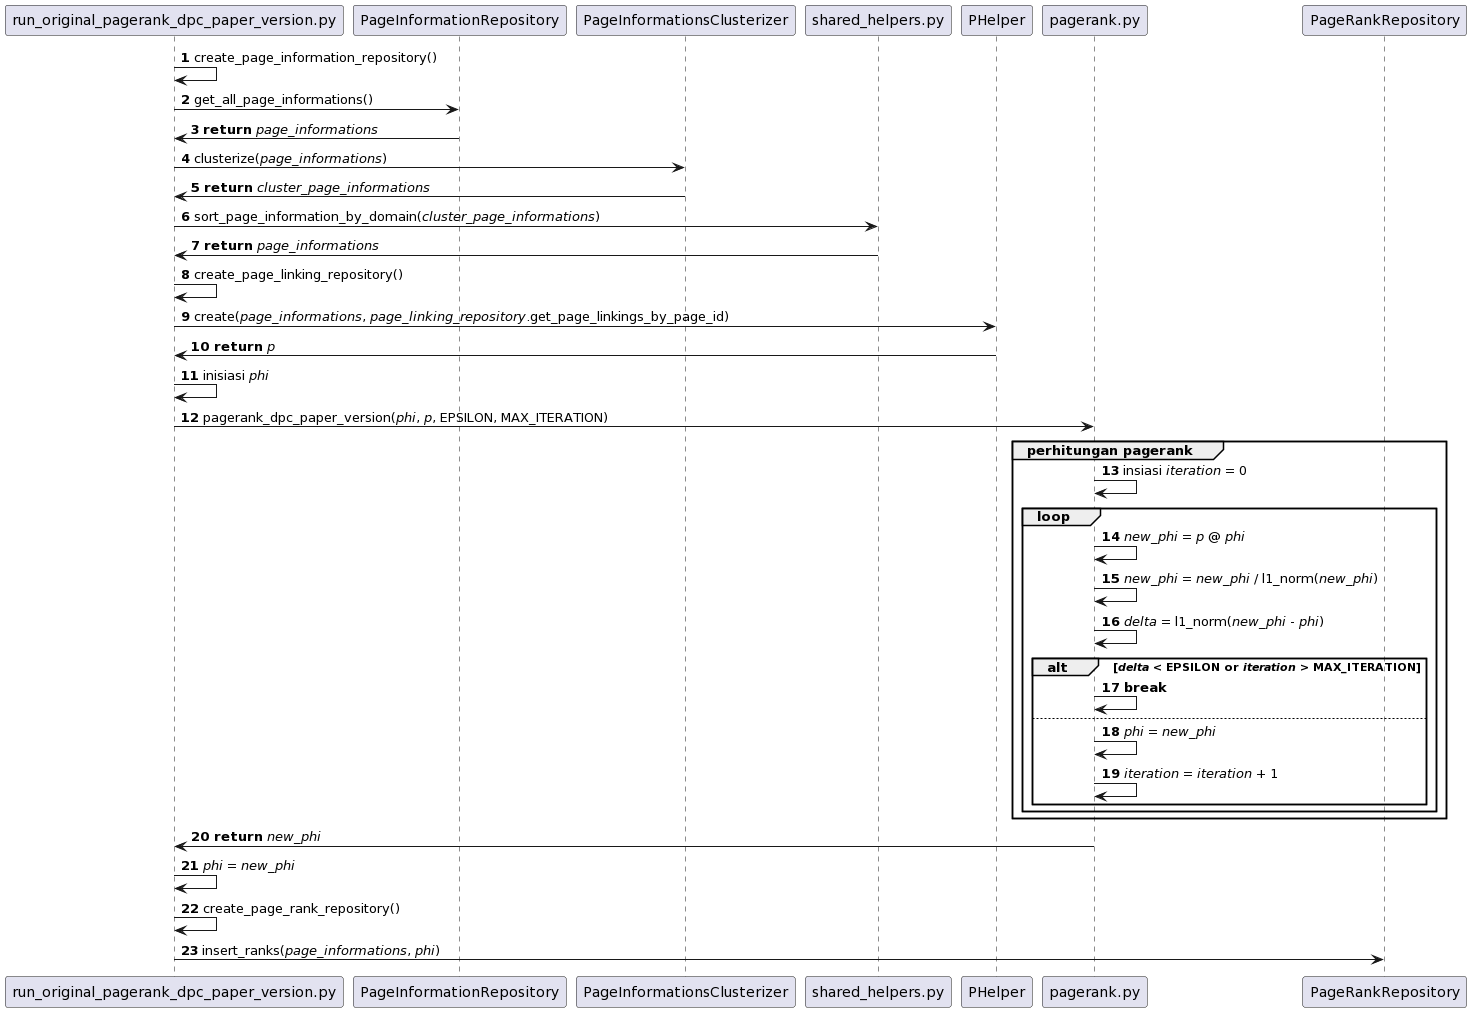
\includegraphics[width={\textheight}, height={\textwidth}, angle=270]{gambar/run_original_pagerank_dpc_paper_version_sequence_diagram}
\caption{Diagram alir dari program Pagerank}
\label{gambar:run_original_pagerank_dpc_paper_version_sequence_diagram}
\end{figure}

\begin{figure}[H]
\centering

\includegraphics[keepaspectratio, width={\textwidth}]{gambar/p_helper_class_diagram(2)}
\caption{\textit{Class Diagram} PHelper}
\label{gambar:p_helper_class_diagram_2}
\end{figure}

Alur kerja dari PHelper dapat dilihat pada diagram alir \ref{gambar:p_helper_sequence_diagram_2}. Kotak abu-abu pada kiri dan kanan diagram menunjukan nama \textit{file} atau \textit{class} terjadinya proses, tanda panah menunjukan perpindahan alur eksekusi dari \textit{file}/\textit{class} yang satu ke yang lainnya, nama di atas panah merupakan nama \textit{method} atau \textit{function} yang dipanggil, kata "\textit{return}" berarti hasil keluaran dari \textit{method}/\textit{function}, kata "\textit{loop}" berarti pengulangan, kata "\textit{alt}" berarti percabangan alur program. Pada langkah satu \textit{method} \textit{create\_p} dipanggil dengan argumen \textit{page\_informations} dan sebuah \textit{method} \textit{PageLinkingRepository.get\_page\_linking\_by\_id}. Pada langkah dua dibuat sebuah \textit{dictionary} yang berisi PageInformation dan \textit{url}-nya sebagai kunci. Selanjutnya pada langkah enam, dilakukan \textit{looping} berdasarkan jumlah banyaknya halaman web yang ada pada \textit{dataset}, proses ini juga dapat dilakukan secara pararel dengan \textit{multi threading}. Pada langkah enam dilakukan pengisian matriks $P$ pada setiap kolomnya. Alasan dilakukan pada tiap kolom karena terdapat nilai yang dipakai secara bersama yaitu banyaknya jumlah \textit{PageLinking} suatu halaman web. Langkah 12 merupakan langkah penting, yaitu perhitungan nilai elemen matriks $P$. Dasar dari perhitungan dari persamaan \ref{eq:5-1}.

\subsection{Program Pagerank}

Alur algoritma Pagerank dalam program dapat dilihat pada gambar \ref{gambar:run_original_pagerank_dpc_paper_version_sequence_diagram}. Langkah satu dilakukan instansiasi PageInformationRepository untuk mengambil semua data dari tabel \textit{page\_information} dari basis data. Selanjutnya pada langkah empat dilakukan klasterisasi dari data \textit{page\_information} untuk dilakukan pengurutan berdasarkan \textit{cluster}-nya. Hal ini dilakukan untuk mempermudah proses pemetaan antara vektor \textit{ranking} halaman web $\pi$ dengan \textit{list} \textit{page\_information}. Pada langkah delapan dilakukan instansiasi PageLinkingRepository untuk membuat matriks transisi $P$ yang memerlukan koneksi basis data untuk memperoleh data dari tabel \textit{page\_linking}. Setelah membuat matriks $P$, pada langkah sepuluh dilakukan inisiasi nilai $\pi$ dan $e$, dan selanjutnya dilakukan perhitungan \textit{pagerank}. Setelah melakukan perhitungan \textit{pagerank}, pada langkah 22 dilakukan instansiasi PagerankRepository, untuk menyimpam hasil perhitungan \textit{pagerank} ke basis data.

\subsection{Program DPC}

\quad Selanjutnya akan dibahas kode program DPC. Berbeda dengan program Pagerank yang cenderung lebih sederhana, perhitungan pada program DPC lebih kompleks. Akibatnya dibutuhkan \textit{class} pendukung yang lebih banyak. Terdapat delapan \textit{class} pendukung yang dipakai oleh program DPC, yaitu ClusterSeparatedPhiHelper, ExtendedLocalTransitionMatrixHelper, PWithCacheHelper, PartitionedPHelper, PastiHelper, PiastHelper, RPHelper, dan DPCExecutor.

ClusterSeparatedPhiHelper merupakan salah satu \textit{helper class} yang berisi \textit{method}-\textit{method} yang berkaitan dengan vektor $\pi$ yang dipecah sesuai dengan \textit{cluster}-nya masing-masing. \textit{Method} \textit{construct\_cluster\_separated\_phi} melakukan perhitungan pada langkah \ref{alg:3.step:trivial:2} pada algoritma DPC, menghitung nilai $\pi$ pada tiap \textit{cluster}. Selanjutnya \textit{method} \textit{flatten\_cluster\_separated\_phi} menyatukan vektor-vektor $\pi$ yang terpisah menjadi ke dalam satu vektor. \textit{Method} \textit{update\_cluster\_separated\_phi} melakukan perhitungan untuk memperbaharui nilai vektor $\pi$ sesuai dengan langkah \ref{alg:3.step:3:3} pada algoritma DPC. Yang terakhir ada \textit{method} \textit{construct\_s} yang membuat sebuah matriks $S$ berdasarkan vektor-vektor $\pi$ yang terpisah berdasarkan \textit{cluster}-nya.

\begin{figure}[H]
  \centering
  
\includegraphics[keepaspectratio, width={\textwidth}]{gambar/cluster_separated_phi_helper_class_diagram}
  \caption{\textit{Class Diagram} ClusterSeparatedPhiHelper}
	\label{gambar:cluster_separated_phi_helper_class_diagram}
\end{figure}

\begin{figure}[H]
  \centering
  
\includegraphics[keepaspectratio, width={\textwidth}]{gambar/extended_local_transition_matrix_helper_class_diagram}
  \caption{\textit{Class Diagram} ExtendedLocalTransitionMatrixHelper}
	\label{gambar:extended_local_transition_matrix_helper_class_diagram}
\end{figure}

ExtendedLocalTransitionMatrixHelper, sesuai namanya, merupakan \textit{helper class} yang berkaitan dengan matriks \textit{extended local transition matrix} yang dalam algoritma DPC berada pada langkah \ref{eq:9}. Pada \textit{method} \textit{construct\_extended\_local\_transition\_matrice} membentuk himpunan matriks $B$ pada setiap \textit{cluster}. Sesuai dengan langkah \ref{eq:9} pada algoritma DPC, \textit{method} ini memuat matriks $P_{ii}$ yang sudah di-\textit{caching} untuk dimasukkan ke beberapa kolom dan baris pertama matriks $B$. Selanjutnya, pada baris paling bawah diisi hasil perkalian vektor $e$ dan matriks $P_{*i}$ yang dimuat dari \textit{class} PastiListCache. Selanjutnya pada kolom paling kanan dilakukan perhitungan yang cukup panjang sesuai pada langkah \ref{eq:9} algoritma DPC. Sel kanan bawah matriks $B$ dapat bernilai apa saja, selama nilai total dari kolom paling kanan matriks $B$ bernilai satu.

Selanjutnya, PWithCacheHelper, sama dengan PHelper, menangani proses pembentukan matriks $P$ tetapi juga menyimpannya ke dalam \textit{disk} atau \textit{caching}. \textit{Class} PWithCacheHelper hanya memiliki satu \textit{public method} yaitu \textit{create\_and\_dump\_p}. Proses pembentukan matriks $P$ pada \textit{class} ini adalah dengan melakukan perhitungan layaknya matriks $P$ pada \textit{class} PHelper tetapi yang membedakan adalah, untuk mengakomodasi matriks yang lebih besar, dilakukan \textit{caching} pada setiap kolom matriksnya.

\begin{figure}[H]
  \centering
  
\includegraphics[keepaspectratio, width={\textwidth}]{gambar/p_with_cache_helper_class_diagram}
  \caption{\textit{Class Diagram} PWithCacheHelper}
\end{figure}

\begin{figure}[H]
  \centering
  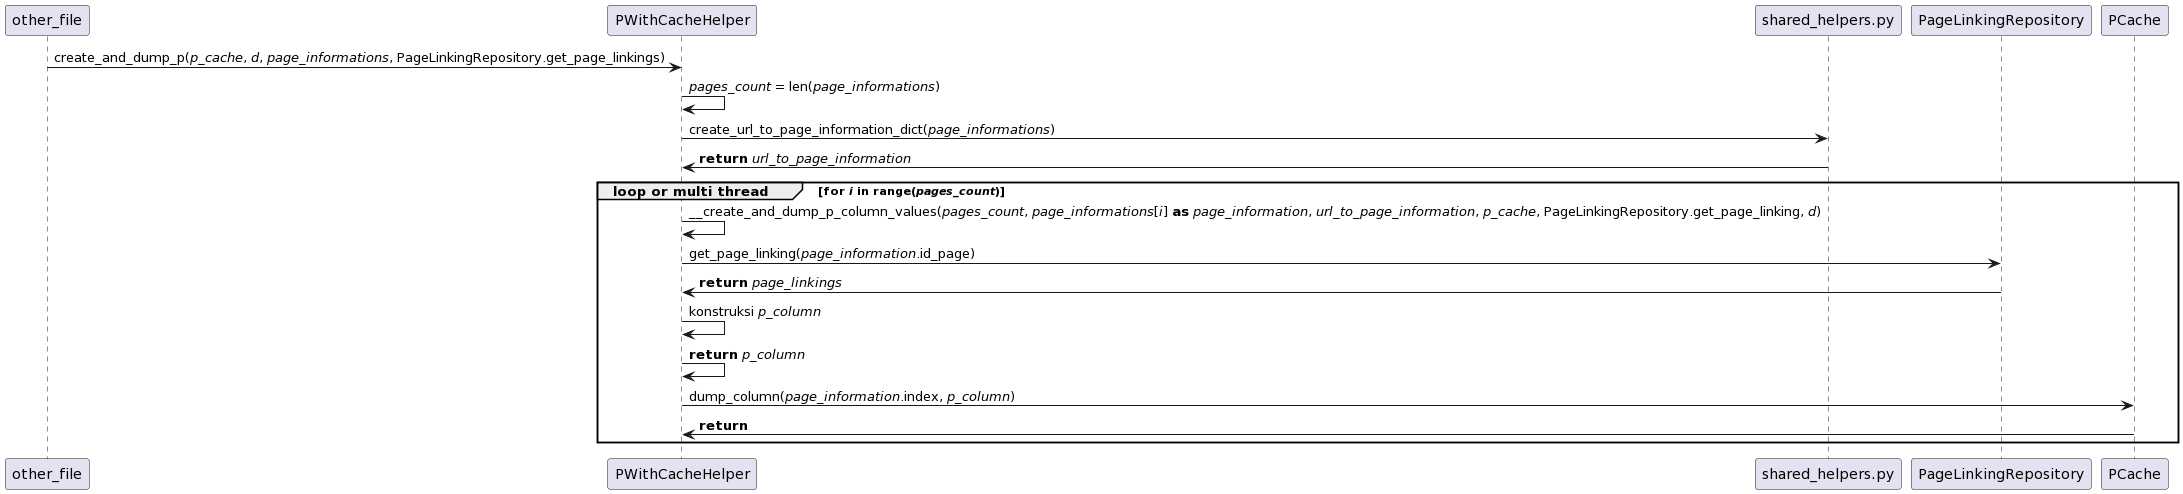
\includegraphics[width={\textwidth}, height={170px}]{gambar/p_with_cache_helper_sequence_diagram}
  \caption{Diagram alir PWithCacheHelper}
\end{figure}

Setelah matriks $P$ terbentuk menggunakan \textit{class} PWithCacheHelper, selanjutnya matriks $P$ dapat dipecah menjadi matriks $P_{ii}$ dan matriks $Q_i$. Matriks $P_{ii}$ mirip dengan matriks $Q_i$ yang merupakan matriks transisi lokal antara halaman web \textit{cluster}-$i$ terhadap \textit{cluster}-$i$, tetapi yang membedakan adalah nilai kolom dari matriks $Q_i$ sudah dinormalisasi. \textit{Class} PartitionedPHelper melalui \textit{method} \textit{dump\_partitioned\_p} memuat kolom-kolom pada matriks $P$ di PCache dipecah menjadi matriks-matriks $P_{ii}$ dimasukkan ke PiiListCache, lalu tiap kolom $P_{ii}$ dinormalisasi menjadi matriks $Q_i$ dan dimasukkan ke dalam QListCache. PiastHelper dan PastiHelper memiliki cara kerja mirip dengan PartitionedPHelper, memuat matriks $P$ dari PCache untuk dibentuk matriks $P_{i*}$ dan matriks $P_{*i}$. 

\begin{figure}[H]
  \centering
  
\includegraphics[keepaspectratio, width={\textwidth}]{gambar/partitioned_p_helper_class_diagram}
  \caption{\textit{Class Diagram} PartitionedPHelper}
	\label{gambar:partitioned_p_helper_class_diagram}
\end{figure}

\begin{figure}[H]
  \centering
  
\includegraphics[keepaspectratio, width={\textwidth}]{gambar/pasti_helper_class_diagram}
  \caption{\textit{Class Diagram} PastiHelper}
	\label{gambar:pasti_helper_class_diagram}
\end{figure}

\begin{figure}[H]
  \centering
  
\includegraphics[keepaspectratio, width={\textwidth}]{gambar/piast_helper_class_diagram}
  \caption{\textit{Class Diagram} PiastHelper}
	\label{gambar:piast_helper_class_diagram}
\end{figure}

RPHelper bertugas menangani perkalian matriks $R$ dan matriks $P$ pada langkah \ref{alg:3.step:2:1} algoritma DPC. Alasan kenapa dibutuhkan \textit{Helper Class} untuk perkalian kedua matriks tersebut, alih-alih menggunakan operator perkalian matriks biasa, karena matriks $P$ memiliki dimensi yang besar dan harus dipecah ke dalam bentuk yang kecil, dalam penelitian ini, matriks $P$ dipecah berdasarkan kolom. Akibatnya, dalam sudut pandang program, perkalian matriks $R$ dan $P$ membutuhkan langkah-langkah kecil. Agar kode lebih rapih langkah-langkah kecil tersebut dimasukkan ke dalam \textit{class} tersendiri. Pada \textit{method} \textit{dump\_and\_mult\_rp} dilakukan \textit{looping} terhadap kolom matriks $RP$ yang nilainya masih kosong, tiap elemen dari kolom $R$ didapatkan dari perkalian antara baris matriks $R$ dan kolom matriks $P$. Hasil perkalian yaitu matriks $RP$ disimpan ke dalam \textit{class} RPCache.

\begin{figure}[H]
	\centering
	
\includegraphics[keepaspectratio, width={\textwidth}]{gambar/rp_helper_class_diagram}
	\caption{\textit{Class Diagram} RPHelper}
	\label{gambar:rp_helper_class_diagram}
\end{figure}	

DPCExecutor merupakan kelas utama yang mengorkestrasi \textit{class} dan fungsi pendukung dalam mengeksekusi program DPC. Terdapat tiga \textit{public method} yang dimiliki DPCExecutor. \textit{insert\_caches} menerima \textit{class} Cache yang sudah diinstansiasi untuk disimpan ke dalam properti DPCExecutor. Selanjutnya, \textit{insert\_helpers} menerima \textit{helper class} yang sudah diinstansiasi untuk disimpan ke dalam properti DPCExecutor. Yang terakhir ada \textit{method execute} yang mengeksekusi program DPC dibantu dengan \textit{cache class} dan \textit{helper class} yang sudah dimasukkan terlebih dahulu.

Sama seperti program Pagerank yang sudah dibahas sebelumnya, program DPC dijalankan dimulai dari sebuah \textit{file} Python, \textit{run\_dpc.py}. Kode dari \textit{run\_dpc.py} dapat dilihat pada kode \ref{listing:run_dpc.py}. Langkah-langkah dari program DPC di \textit{run\_dpc.py} dapat dilihat di gambar \ref{gambar:run_dpc_sequence_diagram}. Langkah pertama dilakukan instansiasi PageInformationRepository untuk mengambil semua data PageInformation di langkah dua. PageInformation yang diambil dari PageInformationRepository, dilakukan klasterisasi pada langkah empat, hasil dari klasterisasi tersebut adalah sebuah klaster dalam bentuk \textit{hashmap}, \textit{key}-nya adalah domain, dan isinya adalah \textit{list} yang berisi PageInformation. Dari data klaster tersebut dapat dilakukan pengurutan \textit{list} PageInformation berdasarkan domain-nya di langkah enam. Selanjutnya pada langkah delapan dilakukan instansiasi PageLinkingRepository untuk mengambil data PageLinking untuk menghitung nilai dari sel matriks transisi $P$ yang dibuat pada langkah sembilan, lalu disimpan ke dalam PCache. Selanjutnya, akan dijalankan algoritma DPC di program melalui DPCExecutor. Setelah dilakukan instansiasi, pada langkah sebelas dan dua belas dimasukkan \textit{cache class} dan \textit{helper class} ke DPCExecutor. Algoritma DPC dijalankan pada langkah 13, yang secara detil dapat dilihat pada gambar \ref{gambar:dpc_executor_sequence_diagram}. Setelah selesai, dikembalikan nilai $\pi$ lalu disimpan ke basis data melalui PagerankRepository.

\begin{figure}[H]
	\centering
	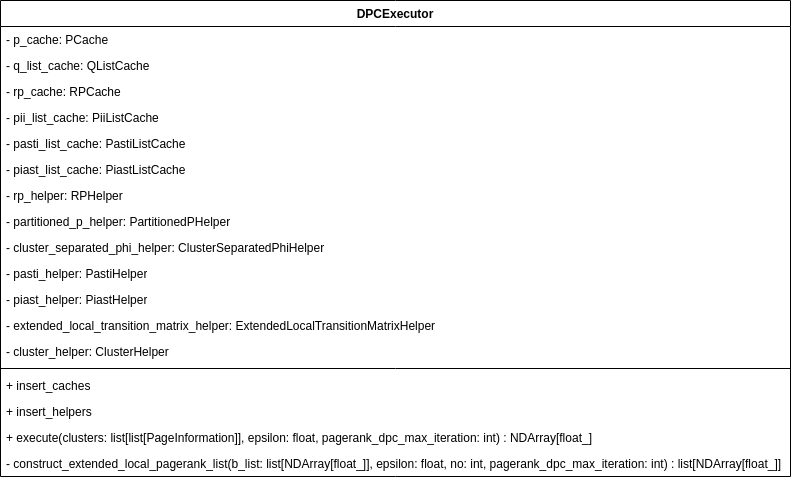
\includegraphics[keepaspectratio, width={\textwidth}]{gambar/dpc_executor_class_diagram}
	\caption{\textit{Class Diagram} DPCExecutor}
	\label{gambar:dpc_executor_class_diagram}
\end{figure}

DPCExecutor dipanggil melalui \textit{method} \textit{execute} dengan memasukan data klaster, $\epsilon$, dan max iterasi. Pertama-tama pada langkah dua sampai lima dengan data klaster dibentuk matriks $R$ dan diperoleh jumlah total halaman. Selanjutnya pada langkah enam dan tujuh, dipartisi nilai matriks $P$ yang diambil dari PCache menjadi himpunan matriks $Q$ dan $P_{ii}$. Lalu pada langkah delapan dan sembilan, dilakukan perhitungan Pagerank pada setiap halaman web yang masih terpisah pada tiap domainnya. Pada langkah sepuluh dan sebelas dilakukan perkalian matriks $R$ dan $P$. Alasan perkalian matriks $R$ dan $P$ dilakukan secara terpisah alih-alih langsung dikalikan dengan matriks $S$, karena dimensi matriks $P$ sangat besar dan nilai matriks $R$ dan $P$ tidak akan berubah, sehingga lebih baik dilakukan secara terpisah terlebih dahulu, dan disimpan ke dalam \textit{cache}. Selanjutnya pada langkah 12 sampai 15 dibentuk matriks $P_{*i}$ dan $P_{i*}$, dengan alasan yang sama dengan matriks $R$ dan $P$ yang nilainya tidak akan berubah. Setelah itu, pada langkah 16 nilai vektor $\pi$ yang masih terpisah pada tiap domainnya, disatukan tanpa ada perubahan nilai. Memasuki \textit{loop} dibentuk matriks $S$ berdasarkan nilai vektor $\pi$ yang masih terpisah terhadap domainnya. Setelah itu, dilakukan perkalian matriks $RP$ dengan matriks $S$ untuk menghasilkan matriks $A$. Matriks $A$ dapat disebut sebagai matriks transisi antara domain/klaster. Pada langkah 25, diperoleh nilai vektor $z$ dengan melakukan perhitungan Pagerank dengan masukan matriks $A$. Vektor $Z$ dapat disebut sebagai \textit{ranking} pada tiap domain. Pada langkah 26 sampai 28 dilakukan \textit{smoothing} dengan membentuk matriks \textit{extended local transition matrix} $B$, dan vektor \textit{extended local pagerank} pada setiap domain-nya. Selanjutnya pada langkah 29 nilai vektor $\pi$ diperbaharui seperti pada langkah \ref{alg:3.step:3:3} algoritma DPC. Setelah itu, nilai $\pi$ dinormalisasi pada langkah 33 dan dihitung nilai delta antara $\pi$ saat ini, dengan $\pi$ iterasi sebelumnya. Jika nilai deltanya kurang dari $\epsilon$, maka perhitungan selesai dan dikembalikan nilai $\pi$ sebagai nilai akhir. Jika tidak, kembali pada langkah awal ketika memasuki \textit{loop}, diawali dengan menambahkan variabel $iteration\_count$ dengan satu untuk menghitung jumlah iterasi yang sudah dilalui. Jumlah iterasi maksimal dapat ditentukan, apabila iterasi tidak kunjung konvergen. Jadi selain nilai delta, jumlah iterasi dapat ditentukan batasnya untuk keluar dari \textit{loop}.

\begin{figure}[H]
\centering
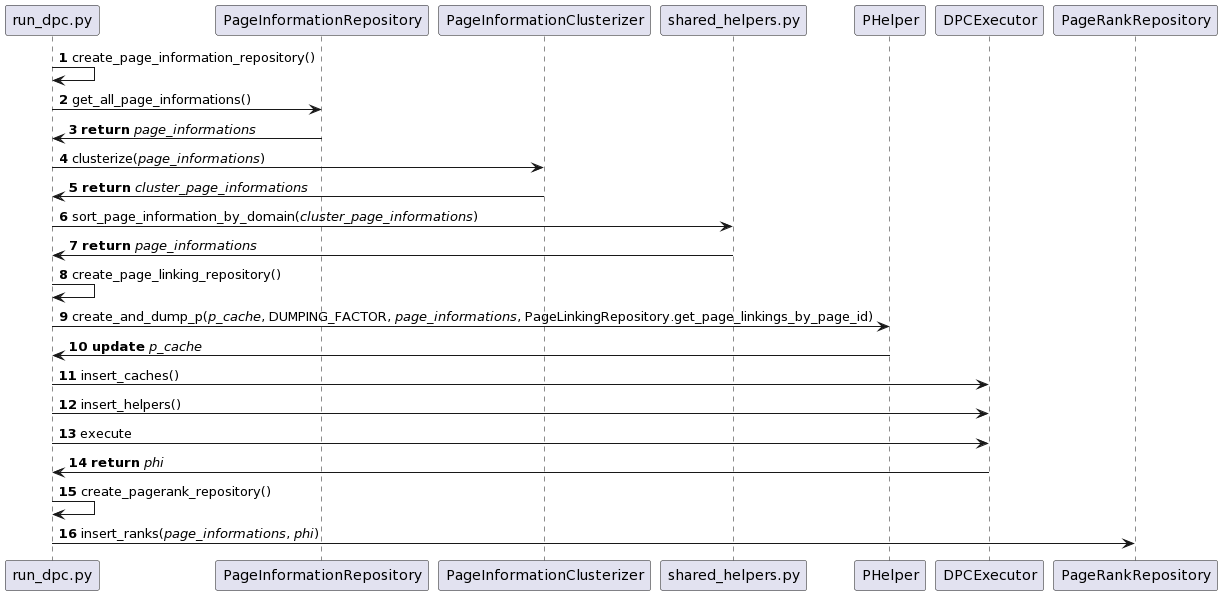
\includegraphics[width={\textheight}, height={\textwidth}, angle=270]{gambar/run_dpc_sequence_diagram}
\caption{Diagram alir \textit{run\_dpc.py}}
\label{gambar:run_dpc_sequence_diagram}
\end{figure}

\begin{figure}[H]
\centering
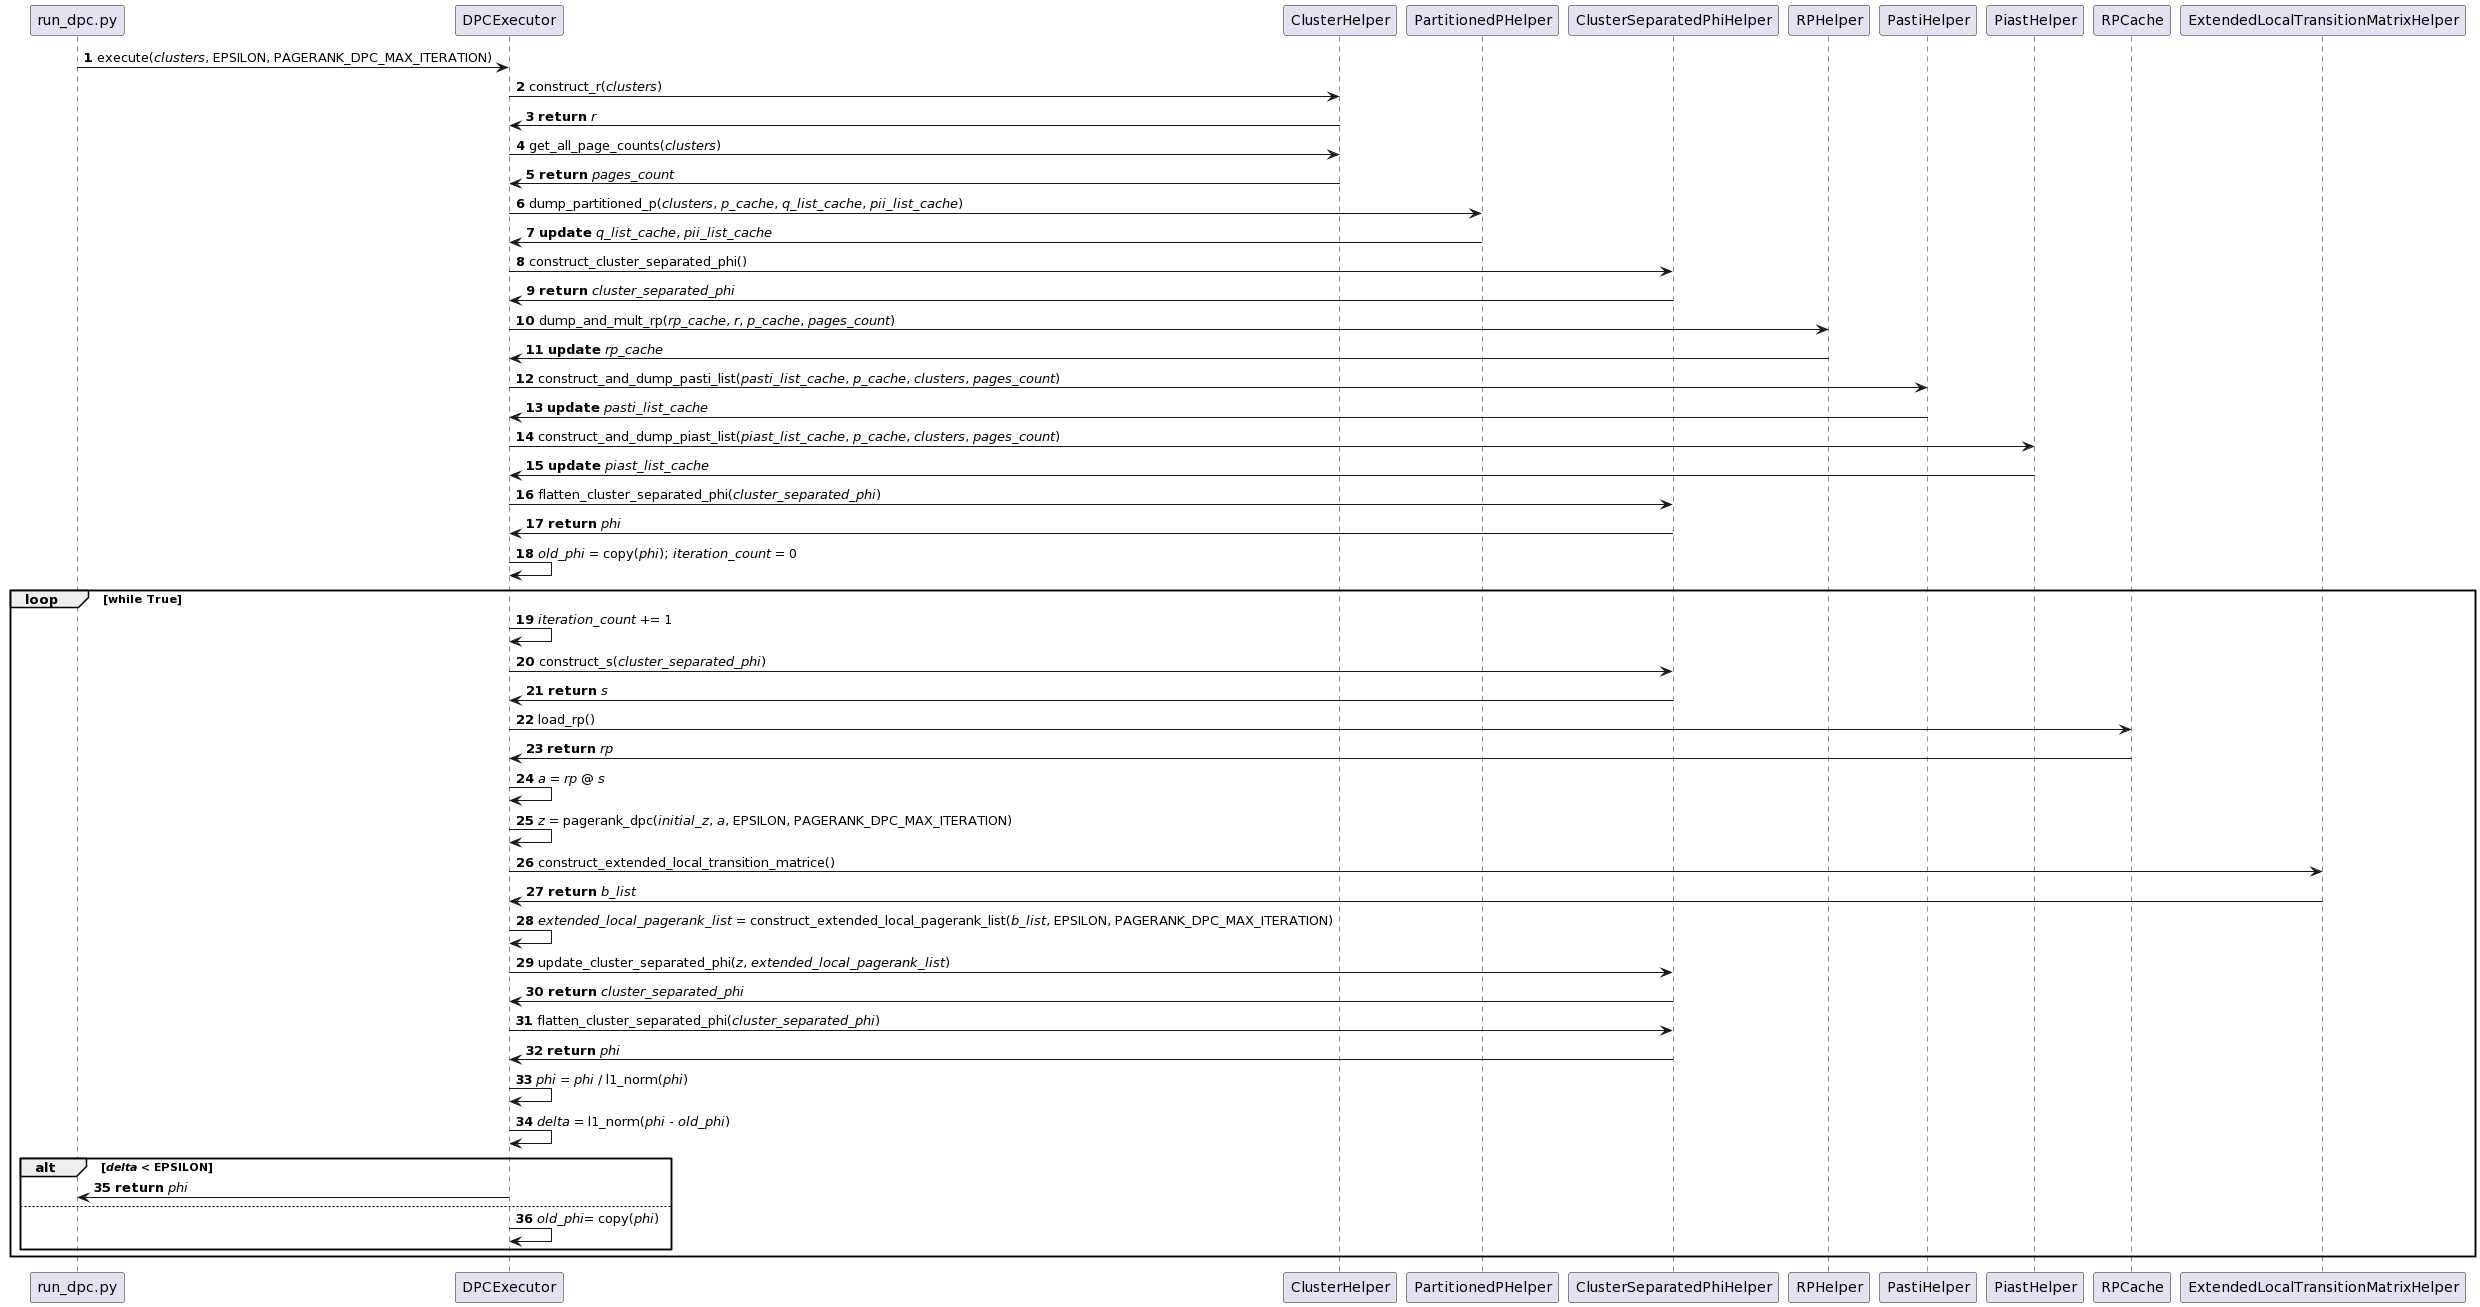
\includegraphics[width={\textheight}, height={\textwidth}, angle=270]{gambar/dpc_executor_sequence_diagram}
\caption{Diagram alir DPCExecutor}
\label{gambar:dpc_executor_sequence_diagram}
\end{figure}

\subsection{Program MDPC}

MDPC merupakan versi lebih sederhana dari algoritma DPC, sehingga kode yang dibuat sangat lebih sedikit dibanding program DPC. Selain itu juga, ada beberapa \textit{class} yang ada pada DPC juga dipakai pada program MDPC. Namun, karena matriks transisi antar \textit{cluster} $A_{mdpc}$ tidak ada pada DPC, maka dibuat \textit{class} AHelper untuk melakukan perhitungan dan membentuk matriks tersebut. Kode program dari \textit{class} AHelper dapat dilihat pada kode \ref{listing:ahelper_class}. Secara garis besar, proses pembentukan matriks $A_{mdpc}$ di \textit{class} ini dimulai dari \textit{public method} \textit{construct\_a}, dilakukan perhitungan nilai pada tiap sel matriks, lalu dilakukan normalisasi pada setiap kolom-nya. Adapun untuk dasar perhitungannya sesuai dengan persamaan \ref{eq:a_mdpc} dan dilakukan pada \textit{method \_\_sum\_sub\_transition\_matrix}.

\begin{figure}[H]
	\centering
	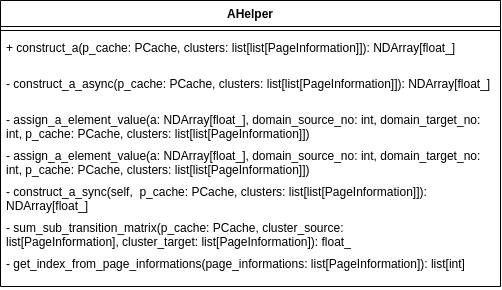
\includegraphics[keepaspectratio, width={\textwidth}]{gambar/a_helper_class_diagram}
	\caption{\textit{Class Diagram} AHelper}
\end{figure}

Selain AHelper, program MDPC juga memiliki \textit{class} ModifiedDPCV2Executor yang berperan sebagai eksekutor dari program MDPC. Secara struktur ModifiedDPCV2Executor mirip dengan \textit{class} DPCExecutor, terdapat \textit{public method insert\_caches, insert\_helpers} dan masing-masing dimulai dari \textit{public method execute}. 

\begin{figure}[H]
	\centering
	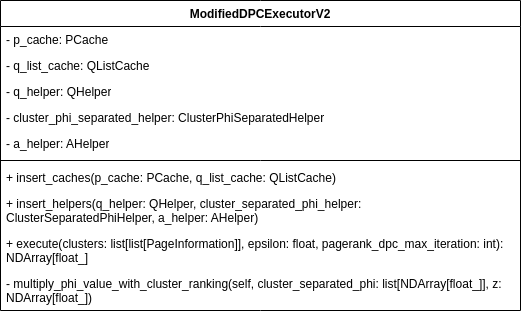
\includegraphics[keepaspectratio, width={\textwidth}]{gambar/modified_dpc_executor_v2_class_diagram}
	\caption{\textit{Class Diagram} ModifiedDPCExecutorV2}
\end{figure}

Ketika \textit{method execute} pada \textit{class} ModifiedDPCV2Executor dipanggil, hal pertama yang dilakukan adalah mengkonstruksi matriks $Q$ dan disimpan ke dalam \textit{cache}. Selanjutnya dilakukan perhitungan \textit{ranking} halaman web atau Pagerank yang masih terisolasi pada setiap domain-nya, di dalam program disimpan ke dalam variabel \textit{cluster\_separated\_phi}, sesuai dengan langkah \ref{alg:mdpc.step.1} algoritma MDPC. Setelah itu dibuat matriks transisi antar \textit{cluster} $A_{mdpc}$ menggunakan \textit{class} AHelper. Selanjutnya dilakukan perhitungan \textit{ranking} tiap \textit{cluster} dengan menggunakan $A_{mdpc}$ sebagai matriks transisi. Setelah diperoleh \textit{cluster ranking}, dilakukan perkalian \textit{ranking} halaman web yang masih terisolasi terhadap \textit{cluster} dengan \textit{cluster ranking}. Nilai Pagerank pada \textit{cluster\_separated\_phi} dianggap tidak terisolasi terhadap \textit{cluster} dan dilakukan penggabungan menjadi sebuah vektor Pagerank tunggal dan dikembalikan sebagai hasil akhir.

\begin{figure}[H]
\centering
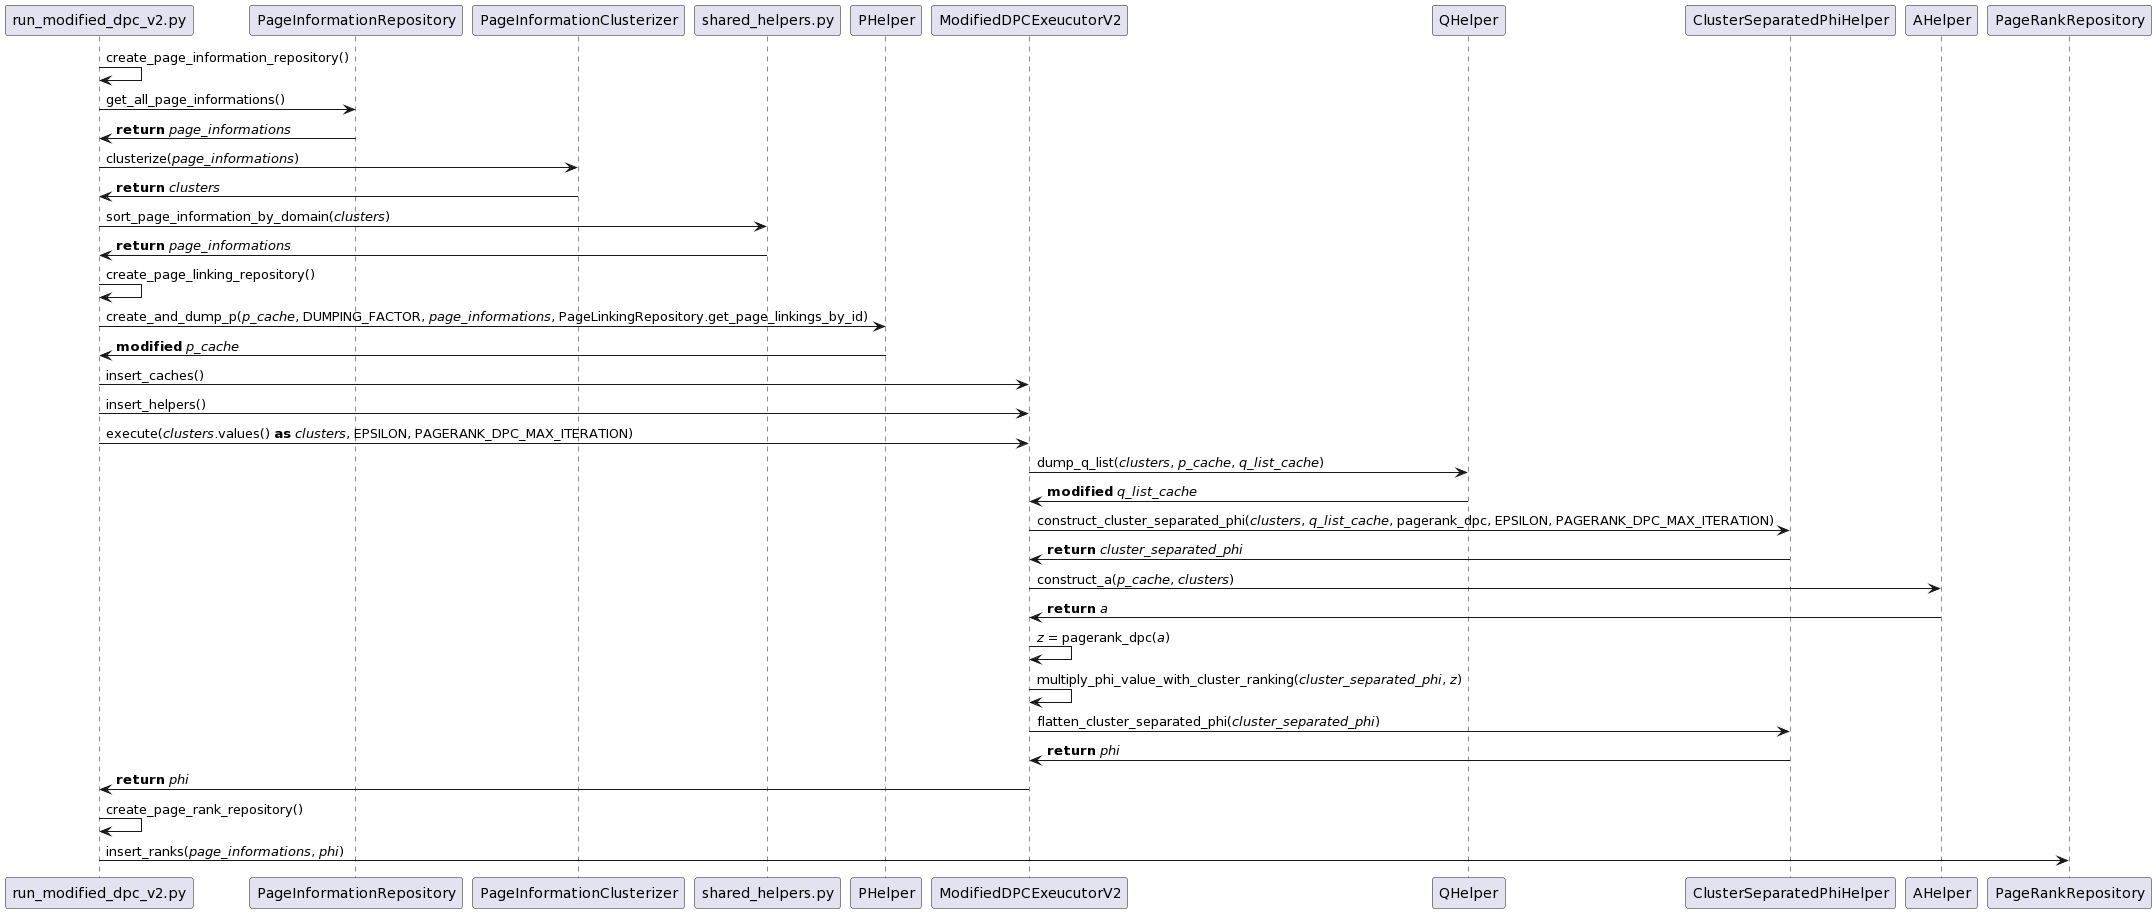
\includegraphics[width={\textheight}, height={\textwidth}, angle=270]{gambar/run_modified_dpc_v2_sequence_diagram}
\caption{Diagram alir program MDPC}
\label{gambar:run_modified_dpc_v2_sequence_diagram}
\end{figure}

Serupa dengan program DPC, program MDPC dimulai dari sebuah \textit{Python file run\_modified\_dpc\_v2.py}. Alur dari program MDPC secara keseluruhan dapat dilihat pada diagram alir gambar \ref{gambar:run_modified_dpc_v2_sequence_diagram}. Sama dengan program-program sebelumnya, langkah awal yaitu instansiasi repositori dan diambil semua data informasi halaman web PageInformation, diklasterisasi, diurutkan, dan lalu dapat dibentuk matriks $P$ yang disimpan ke dalam PCache. Selanjutnya dilakukan instansiasi \textit{cache class} dan \textit{helper class} lain lalu dimasukkan ke dalam ekskutor ModifiedDPCExecutorV2. Selanjutnya dipanggil \textit{public method execute}. Setelah diperoleh nilai $\pi$, lalu disimpan ke basis data melalui PagerankRepository.

\subsection{Program Random Walker}

\begin{figure}[H]
	\centering
	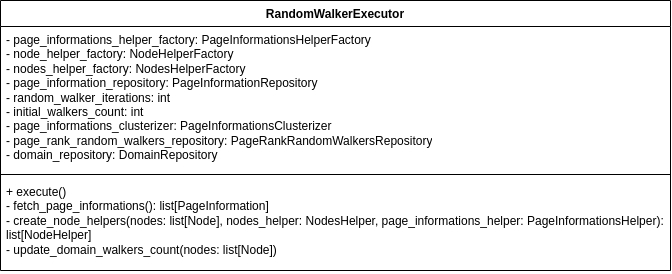
\includegraphics[keepaspectratio, width={\textwidth}]{gambar/random_walker_executor_class_diagram}
	\caption{\textit{Class Diagram} RandomWalkerExecutor}
\end{figure}

Program Random Walker merupakan sebuah simulasi dari Pagerank. Secara program, Random Walker memiliki sebuah \textit{executor class} dan beberapa \textit{factory helper} dan \textit{helper class}. Program dimulai dengan menjalankan berkas Python \textit{run\_random\_walker.py}. Berkas Python tersebut memanggil \textit{method} \textit{execute} pada \textit{class} RandomWalkerExecutor. Pertama, diambil data semua PageInformation di basis data melalui PageInformationRepository. Selanjutnya, tiap PageInformation disimpan ke dalam \textit{class} Node. Node memiliki properti \textit{page\_information}, \textit{walkers\_count} untuk menampung jumlah \textit{walker} yang berada di Node saat ini, dan \textit{next\_walkers\_count} untuk menampung jumlah \textit{walker} yang berada di Node pada iterasi selanjutnya.

\begin{figure}[H]
	\centering
	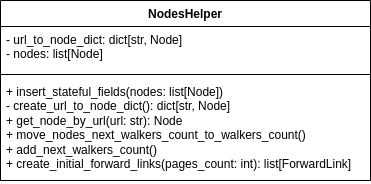
\includegraphics[keepaspectratio, width={0.55\textwidth}]{gambar/nodes_helper_class_diagram}
	\caption{\textit{Class Diagram} NodesHelper}
\end{figure}

\begin{figure}[H]
	\centering
	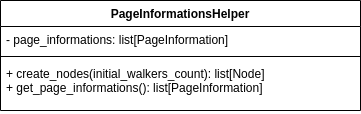
\includegraphics[keepaspectratio, width={0.55\textwidth}]{gambar/page_informations_helper_class_diagram}
	\caption{\textit{Class Diagram} PageInformationsHelper}
\end{figure}

Sebelum memasuki langkah iterasi, akan dilakukan iterasi sebanyak yang ditentukan, pada penelitian ini jumlah iterasinya adalah 20 iterasi. Memasuki iterasi, untuk setiap Node, diambil Node tujuan, dan probabilitas setiap Node tujuan. Melalui fungsi \textit{random.choices} dimasukkan jumlah \textit{walker}, \textit{list} Node tujuan, dan \textit{list} probabilitas Node tujuan. Keluaran dari fungsi \textit{random.choices} adalah \textit{list} Node dari Node tujuan sebanyak jumlah \textit{walker}, yang dianggap sebagai Node tujuan terpilih pada setiap \textit{walker}. Pada setiap Node terpilih dilakukan penambahan nilai \textit{next\_walker\_count} sebanyak satu. Setelah satu iterasi selesai, nilai \textit{walkers\_count} di-perbaharui dengan memindahkan nilai \textit{next\_walkers\_count} ke \textit{walkers\_count}. Langkah pada iterasi diulangi, sampai iterasi selesai. Penjelasan program dapat dilihat dalam bentuk diagram alir pada gambar \ref{gambar:random_walker_sequence_diagram}.

\begin{figure}[H]
	\centering
	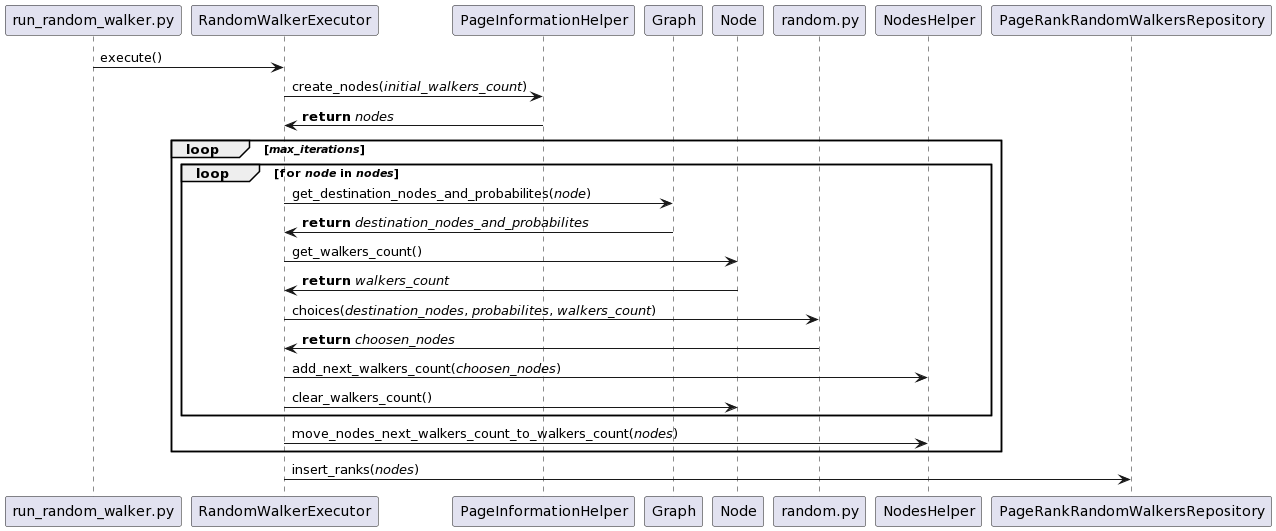
\includegraphics[width={\textheight}, height={\textwidth}, angle=270]{gambar/run_random_walker_sequence_diagram}
	\caption{Diagram alir program Random Walker}
	\label{gambar:random_walker_sequence_diagram}
\end{figure}

\section{Hasil}

Setelah program dijalankan terhadap semua \textit{dataset}, maka diperoleh hasil berikut. Pada Dataset 2 puncak penggunaan memori pada ketiga algoritma relatif sama, hal ini dikarenakan data yang cukup kecil dibandingkan \textit{overhead} memory pada program. Selanjutnya pada Dataset 1 puncak penggunaan memori terbesar ada pada algoritma pagerank asli yaitu sebesar 3,4 GB dimulai saat matriks $20.493\times 20.493$ $P$ dibentuk. Dengan perhitungan setiap sel matriks merupakan angka desimal \textit{floating point} 64bit maka besarnya matriks $P$ pada memori adalah $\pm$3,4 GB. 

Selanjutnya, pada algoritma DPC penggunaan memori terbesar adalah 842 MB yang terjadi pada pembentukan dan penyimpanan matriks $P_{*i}$ ke \textit{cache}. Mengingat domain terbesar di Dataset 1 yaitu "detik.com" dengan jumlah 2.215 halaman, maka dimensi matriks $P_{*i}$ terbesar adalah $20.493 \times 2.215$ yang akan memakan memori sebesar $\pm363$ MB, dan ketika akan disimpan ke dalam \textit{cache} menggunakan \textit{pickle library} akan dilakukan penyalinan objek sebelum ditulis ke dalam \textit{cache}, sehingga penggunaan memori $2 \times \pm363 MB = \pm726 MB$. 

Pada algoritma MDPC puncak memori sebesar $\pm86$ MB, penggunaan memori puncak terjadi pada langkah pembentukan dan penyimpanan matriks $Q$ ke \textit{cache}. Karena matriks $Q$ adalah matriks transisi lokal suatu domain, maka matriks $Q$ terbesar adalah matriks $Q$ domain "detik.com" dengan 2.215 halaman. Ukuran matriks $Q$ yang terbentuk adalah $2.215 \times 2.215$ yang secara ukuran di memori adalah $\pm39$ MB, dan di tengah proses penyimpanan ke dalam \textit{cache} dilakukan penyalinan objek sementara, sehingga ukuran memorinya menjadi dua kali lipat yaitu $\pm86$ MB. Perbandingan puncak memori dan lamanya waktu eksekusi algoritma Pagerank Original, algoritma Distributed Pagerank Computation (DPC), dan algoritma Modified DPC (MDPC), dapat dilihat pada tabel \ref{table:algorithm_performance}.

\begin{longtable}{|c|c|c|}
	\caption{Puncak penggunaan memori dan waktu eksekusi}
	\label{table:algorithm_performance} \\
	\hline
	\textbf{Algoritma} & \textbf{Puncak Penggunaan Memori(\textit{Mega Byte})} & \textbf{Waktu(Detik)} \\
	\hline
	\multicolumn{3}{|c|}{Dataset 1 (20.493 halaman)} \\
	\hline
	Pagerank & 3.417,63239 & 328,803 \\
	DPC & 842,48153 & 1.151,628 \\
	MDPC & 86,58194 & 816,375 \\
	\hline
	\multicolumn{3}{|c|}{Dataset 2 (100 halaman)} \\
	\hline
	Pagerank & 2,04511 & 0,568 \\
	DPC & 2,0563 & 19,372 \\
	MDPC & 2,05595 & 0,652 \\
	\hline
\end{longtable}

Selanjutnya akan dihitung nilai kemiripan antara nilai Pagerank yang dihasilkan program Pagerank asli, DPC, MDPC, dan Random Walker. Nilai Pagerank berbentuk vektor dan diurutkan berdasarkan \textit{id} halaman. Pada Dataset 1, nilai $KDist$ tiap vektor \textit{ranking} halaman web yang dihasilkan oleh algoritma Pagerank, DPC, MDPC, dan Random Walker dapat dilihat pada tabel \ref{table:kendall_distance_score_dataset_1}. 

\begin{longtable}{|c|c|c|c|c|}
	\caption{Nilai jarak Kendall vektor Pagerank pada dataset 1 (20.493 halaman)}
	\label{table:kendall_distance_score_dataset_1} \\
	\hline
	& \textbf{Pagerank} & \textbf{DPC} & \textbf{MDPC} & \textbf{Random Walker} \\
	\hline
	\textbf{Pagerank} & 0,0 & 0,24956 & 0,25985 & 0,02716 \\
	\hline
	\textbf{DPC} & 0,24956 & 0,0 & 0,27681 & 0,25208 \\
	\hline
	\textbf{MDPC} & 0,25985 & 0,27681 & 0,0 & 0,26387 \\
	\hline
	\textbf{Random Walker} & 0,02716 & 0,25208 & 0,26387 & 0,0 \\
	\hline
\end{longtable}

Vektor yang paling mirip atau memiliki nilai $KDist$ terkecil adalah vektor Pagerank dan Random Walker yaitu sebesar $0,02716$ atau $2,7$ persen perbedaan urutan. Sedangkan $KDist$ untuk DPC terhadap Pagerank dan Random Walker secara berurutan adalah $0,24956$ dan $0,25208$ atau $25$ persen dan $25,2$ persen perbedaan urutan. Selanjutnya untuk $KDist$ MDPC terhadap DPC, Pagerank, dan Random Walker secara berurutan adalah $0,27681$, $0,25985$, dan $0,26387$ atau $27,7$ persen, $26$ persen, dan $26,4$ persen perbedaan urutan.

Pada Dataset 2, nilai $KDist$ tiap vektor \textit{ranking} halaman web yang dihasilkan oleh algoritma Pagerank, DPC, MDPC, dan Random Walker dapat dilihat pada tabel \ref{table:kendall_distance_score_dataset_2}. Vektor yang paling mirip atau memiliki nilai $KDist$ terkecil adalah vektor Pagerank dan Random Walker yaitu sebesar $0,03293$ atau $3,3$ persen perbedaan urutan. Sedangkan $KDist$ untuk DPC terhadap Pagerank dan Random Walker secara berurutan adalah $0,17131$ dan $0,19131$ atau $17,1$ persen dan $19,1$ persen perbedaan urutan. Selanjutnya untuk $KDist$ MDPC terhadap DPC, Pagerank, dan Random Walker secara berurutan adalah $0,11091$, $0,12586$, dan $0,14949$ atau $11,1$ persen, $12,6$ persen, dan $14,9$ persen perbedaan urutan.

\begin{longtable}{|c|c|c|c|c|}
	\caption{Nilai jarak Kendall vektor Pagerank pada dataset 2 (100 halaman)}
	\label{table:kendall_distance_score_dataset_2} \\
	\hline
	& \textbf{Pagerank} & \textbf{DPC} & \textbf{MDPC} & \textbf{Random Walker} \\
	\hline
	\textbf{Pagerank} & 0,0 & 0,17131 & 0,12586 & 0,03293 \\
	\hline
	\textbf{DPC} & 0,17131 & 0,0 & 0,11091 & 0,19131 \\
	\hline
	\textbf{MDPC} & 0,12586 & 0,11091 & 0,0 & 0,14949 \\
	\hline
	\textbf{Random Walker} & 0,03293 & 0,19131 & 0,14949 & 0,0 \\
	\hline
\end{longtable}

Secara lebih detil, perbedaan peringkat halaman satu per satu berdasarkan tiap algoritmanya dapat dilihat pada tabel \ref{table:rank_comparisson_dataset_1} untuk Dataset 1, dan tabel \ref{table:rank_comparisson_dataset_2} untuk Dataset 2. Kolom \textit{Rank} menunjukan urutan peringkat halaman web, nilai pada kolom \textit{value} merupakan nilai dari peringkat halaman web yang merupakan nilai peluang ($0 \leq \text{\textit{value}} \leq 1$), dan pada nilai pada kolom \textit{page\_id} merupakan nomor pembeda atau \textit{Primary Key} yang disematkan pada basis data relasional.

\begin{longtable}{|c|c|c|c|c|}
	\caption{Perbandingan peringkat halaman web Dataset 1 (20.493 halaman) bag. 1}
	\label{table:rank_comparisson_dataset_1} \\
	\hline
	\multicolumn{5}{|c|}{Dataset 1 (20.493 halaman)} \\
	\hline
	& \multicolumn{2}{c|}{Pagerank} & \multicolumn{2}{c|}{DPC} \\
	\hline
	\textbf{Rank} & \textbf{\textit{page\_id}} & \textbf{\textit{value}} & \textbf{\textit{page\_id}} & \textbf{\textit{value}} \\
	\hline
	1 & 13.343 & 0,00975 & 9.262 & 0,00489 \\
	2 & 2.858 & 0,0093 & 9.276 & 0,00489 \\
	3 & 11.365 & 0,00635 & 9.285 & 0,00489 \\
	4 & 18.179 & 0,0048 & 16.214 & 0,00489 \\
	5 & 7 & 0,00465 & 16.217 & 0,00489 \\
	$\vdots$ & $\vdots$ & $\vdots$ & $\vdots$ & $\vdots$ \\
	20.489 & 13.012 & 0,00001 & 1.654 & 0,0 \\
	20.490 & 13.015 & 0,00001 & 1.656 & 0,0 \\
	20.491 & 13.004 & 0,00001 & 1.655 & 0,0 \\
	20.492 & 13.005 & 0,00001 & 1.653 & 0,0 \\
	20.493 & 10.723 & 0,00001 & 1.658 & 0,0 \\
	\hline
\end{longtable}

\begin{longtable}{|c|c|c|c|c|}
	\caption{Perbandingan peringkat halaman web Dataset 1 (20.493 halaman) bag. 2}
	\label{table:rank_comparisson_dataset_1} \\
	\hline
	\multicolumn{5}{|c|}{Dataset 1 (20.493 halaman)} \\
	\hline
	& \multicolumn{2}{c|}{MDPC} & \multicolumn{2}{c|}{Random Walker} \\
	\hline
	\textbf{Rank} & \textbf{\textit{page\_id}} & \textbf{\textit{value}} & \textbf{\textit{page\_id}} & \textbf{\textit{value}} \\
	\hline
	1 & 2.087 & 0,01244 & 13.343 & 0,00966 \\
	2 & 13.343 & 0,00985 & 2.858 & 0,00933 \\
	3 & 2.858 & 0,0093 & 11.365 & 0,00621 \\
	4 & 2.859 & 0,00718 & 18.179 & 0,00483 \\
	5 & 699 & 0,00654 & 7 & 0,00466 \\
	\hline
	\hline
	\multicolumn{5}{|c|}{Dataset 1 (20.493 halaman)} \\
	\hline
	& \multicolumn{2}{c|}{MDPC} & \multicolumn{2}{c|}{Random Walker} \\
	\hline
	\textbf{Rank} & \textbf{\textit{page\_id}} & \textbf{\textit{value}} & \textbf{\textit{page\_id}} & \textbf{\textit{value}} \\
	\hline
	$\vdots$ & $\vdots$ & $\vdots$ & $\vdots$ & $\vdots$ \\
	20.489 & 16.464 & 0,0 & 9.192 & 0,00001 \\
	20.490 & 16.504 & 0,0 & 9.167 & 0,00001 \\
	20.491 & 15.644 & 0,0 & 16.005 & 0,00001 \\
	20.492 & 13.898 & 0,0 & 9.179 & 0,00001 \\
	20.493 & 16.347 & 0,0 & 15.866 & 0,00001 \\
	\hline
\end{longtable}

\begin{longtable}{|c|c|c|c|c|}
	\caption{Perbandingan peringkat halaman web Dataset 2 (100 halaman) bag. 1}
	\label{table:rank_comparisson_dataset_2} \\
	\hline
	\multicolumn{5}{|c|}{Dataset 2 (100 halaman)} \\
	\hline
	& \multicolumn{2}{c|}{Pagerank} & \multicolumn{2}{c|}{DPC} \\
	\hline
	\textbf{Rank} & \textbf{\textit{page\_id}} & \textbf{\textit{value}} & \textbf{\textit{page\_id}} & \textbf{\textit{value}} \\
	1 & 72 & 0,08431 & 72 & 0,1306 \\
	2 & 62 & 0,01856 & 95 & 0,02583 \\
	3 & 54 & 0,01856 & 91 & 0,02583 \\
	4 & 55 & 0,01856 & 87 & 0,02583 \\
	5 & 59 & 0,01856 & 97 & 0,02583 \\
	$\vdots$ & $\vdots$ & $\vdots$ & $\vdots$ & $\vdots$ \\
	96 & 63 & 0,00199 & 1 & 0,00043 \\
	97 & 64 & 0,00199 & 25 & 0,00037 \\
	98 & 80 & 0,00199 & 63 & 0,00037 \\
	99 & 28 & 0,00184 & 64 & 0,00037 \\
	100 & 1 & 0,0015 & 80 & 0,00037 \\
	\hline
\end{longtable}

\begin{longtable}{|c|c|c|c|c|}
	\caption{Perbandingan peringkat halaman web Dataset 2 (100 halaman) bag. 2}
	\label{table:rank_comparisson_dataset_2} \\
	\hline
	\multicolumn{5}{|c|}{Dataset 2 (100 halaman)} \\
	\hline
	& \multicolumn{2}{c|}{MDPC} & \multicolumn{2}{c|}{Random Walker} \\
	\hline
	\textbf{Rank} & \textbf{\textit{page\_id}} & \textbf{\textit{value}} & \textbf{\textit{page\_id}} & \textbf{\textit{value}} \\
	\hline
	1 & 72 & 0,16809 & 72 & 0,08381 \\
	2 & 54 & 0,03158 & 54 & 0,01856 \\
	3 & 55 & 0,03158 & 62 & 0,01847 \\
	4 & 59 & 0,03158 & 55 & 0,01847 \\
	5 & 62 & 0,03158 & 59 & 0,01842 \\
	$\vdots$ & $\vdots$ & $\vdots$ & $\vdots$ & $\vdots$ \\
	96 & 25 & 0,00048 & 80 & 0,002 \\
	97 & 63 & 0,00048 & 63 & 0,00198 \\
	98 & 64 & 0,00048 & 64 & 0,00197 \\
	99 & 80 & 0,00048 & 28 & 0,0018 \\
	100 & 1 & 0,00022 & 1 & 0,00151 \\
	\hline
\end{longtable}

Selain perbedaan nilai peringkat, perbedaan selisih nilai atau hasil pengurangan antara pada setiap halaman web antara algoritma satu dengan yang lainnya dapat dilihat pada tabel \ref{table:rank_value_difference_dataset_1_part_1} dan tabel \ref{table:rank_value_difference_dataset_1_part_2} untuk Dataset 1, dan tabel \ref{table:rank_value_difference_dataset_2_part_1} dan tabel \ref{table:rank_value_difference_dataset_2_part_2} untuk Dataset 2. Mengetahui perbedaan selisih nilai penting untuk mengetahui seberapa jauh deviasi atau perubahan hasil nilai \textit{ranking} antara keempat algoritma (Pagerank Original, DPC, MDPC, dan Random Walker). Semakin besar nilai selisihnya, semakin besar pula perbedaannya. Hal ini juga merupakan keniscayaan karena perbedaan algoritma yang dipakai. Namun, umumnya, selisih yang dibawah $10^{-5}$ dapat ditoleransi dan dianggap sama. Oleh karena itu nilai yang ditampilkan di tabel hanya lima angka desimal, atau lima angka di belakang koma.
 
\begin{longtable}{|c|c|c|c|}
	\caption{Selisih nilai peringkat halaman web Dataset 1 (20.493 halaman) Bagian 1}
	\label{table:rank_value_difference_dataset_1_part_1} \\
	\hline
	\multicolumn{4}{|c|}{Dataset 1 (20.493 halaman)} \\
	\hline
	\textbf{\textit{page\_id}} & \textbf{Pagerank - DPC} & \textbf{Pagerank - MDPC} & \textbf{DPC - MDPC} \\
	\hline
	1 & 0,00002 & 0,00001 & 0,0  \\
	2 & 0,00245 & 0,00008 & 0,00237  \\
	3 & 0,00245 & 0,00008 & 0,00237  \\
	4 & 0,00251 & 0,00217 & 0,00034  \\
	5 & 0,00244 & 0,0019 & 0,00054  \\
	$\vdots$ & $\vdots$ & $\vdots$ & $\vdots$ \\
	20.490 & 0,00006 & 0,00001 & 0,00005  \\
	20.491 & 0,00003 & 0,00003 & 0,0  \\
	20.492 & 0,00003 & 0,00003 & 0,0  \\
	20.493 & 0,00006 & 0,00001 & 0,00005  \\
	20.494 & 0,00003 & 0,00003 & 0,0  \\
	\hline
\end{longtable}

\begin{longtable}{|c|c|c|c|}
	\caption{Selisih nilai peringkat halaman web Dataset 1 (20.493 halaman) bagian 2. Ket: Random Walker (RW)}
	\label{table:rank_value_difference_dataset_1_part_2} \\
	\hline
	\multicolumn{4}{|c|}{Dataset 1 (20.493 halaman)} \\
	\hline
	\textbf{\textit{page\_id}} & \textbf{RW - Pagerank} & \textbf{RW - DPC} & \textbf{RW - MDPC} \\
	\hline
	1 & 0,0 & 0,00002 & 0,00001  \\
	2 & 0,00001 & 0,00246 & 0,00009  \\
	3 & 0,0 & 0,00246 & 0,00008  \\
	4 & 0,00001 & 0,00252 & 0,00218  \\
	5 & 0,0 & 0,00244 & 0,0019  \\
	$\vdots$ & $\vdots$ & $\vdots$ & $\vdots$ \\
	\hline
	\hline
	\multicolumn{4}{|c|}{Dataset 1 (20.493 halaman)} \\
	\hline
	\textbf{\textit{page\_id}} & \textbf{RW - Pagerank} & \textbf{RW - DPC} & \textbf{RW - MDPC} \\
	\hline
	20.490 & 0,0 & 0,00005 & 0,0  \\
	20.491 & 0,0 & 0,00003 & 0,00003  \\
	20.492 & 0,0 & 0,00003 & 0,00003  \\
	20.493 & 0,0 & 0,00005 & 0,0  \\
	20.494 & 0,0 & 0,00003 & 0,00003  \\
	\hline
\end{longtable}

Selanjutnya akan ditampilkan perbedaan selisih keempat algoritma pada Dataset 2 yang berisi 100 halaman web. Sama dengan tabel untuk Dataset 1, angka yang ditampilkan di bawah hanya lima angka di belakang koma.

\begin{longtable}{|c|c|c|c|}
	\caption{Selisih nilai peringkat halaman web Dataset 2 (100 halaman) bagian 1}
	\label{table:rank_value_difference_dataset_2_part_1} \\
	\hline
	\multicolumn{4}{|c|}{Dataset 2 (100 halaman)} \\
	\hline
	\textbf{\textit{page\_id}} & \textbf{Pagerank - DPC} & \textbf{Pagerank - MDPC} & \textbf{DPC - MDPC} \\
	\hline
	1 & 0,00107 & 0,00128 & 0,00021  \\
	2 & 0,00088 & 0,00112 & 0,00024  \\
	3 & 0,00156 & 0,00314 & 0,0047  \\
	4 & 0,00571 & 0,00079 & 0,00492  \\
	5 & 0,00571 & 0,00079 & 0,00492  \\
	$\vdots$ & $\vdots$ & $\vdots$ & $\vdots$ \\
	96 & 0,00269 & 0,00257 & 0,00012  \\
	97 & 0,00784 & 0,00038 & 0,00746  \\
	98 & 0,00328 & 0,00482 & 0,0081  \\
	99 & 0,00328 & 0,00348 & 0,0002  \\
	100 & 0,00277 & 0,00244 & 0,00033  \\
	\hline
\end{longtable}

\begin{longtable}{|c|c|c|c|}
	\caption{Selisih nilai peringkat halaman web Dataset 2 (100 halaman) bagian 2. Ket: Random Walker (RW)}
	\label{table:rank_value_difference_dataset_2_part_2} \\
	\hline
	\multicolumn{4}{|c|}{Dataset 2 (100 halaman)} \\
	\hline
	\textbf{\textit{page\_id}} & \textbf{RW - Pagerank} & \textbf{RW - DPC} & \textbf{RW - MDPC} \\
	\hline
	1 & 0,00001 & 0,00108 & 0,00128  \\
	2 & 0,00001 & 0,00089 & 0,00113  \\
	3 & 0,00001 & 0,00157 & 0,00313  \\
	4 & 0,00004 & 0,00576 & 0,00083  \\
	5 & 0,00008 & 0,00563 & 0,00071  \\
	$\vdots$ & $\vdots$ & $\vdots$ & $\vdots$ \\
	96 & 0,00004 & 0,00266 & 0,00253  \\
	97 & 0,00004 & 0,0078 & 0,00033  \\
	98 & 0,00001 & 0,00327 & 0,00483  \\
	99 & 0,00008 & 0,00336 & 0,00356  \\
	100 & 0,0 & 0,00278 & 0,00244  \\
	\hline
\end{longtable}

Perbedaan hasil cukup signifikan antara Distributed Pagerank Computation (DPC) dan Modified DPC (MDPC) terhadap Pagerank Original dan Random Walker disebabkan karena dasar dari perhitungannya yang berbeda. DPC dan MDPC memisahkan halaman web berdasarkan domain-nya, sedangkan Pagerank dan Random Walker melakukan perhitungan secara utuh.

Dapat disimpulkan, algoritma Pagerank Original paling cepat dan paling mirip hasilnya dengan algoritma Random Walker dalam melakukan pe-\textit{ranking}-an halaman web, namun memerlukan memori utama yang lebih besar. Sedangkan algoritma DPC dan MDPC memerlukan memori utama lebih kecil, sehingga cocok untuk komputer satu mesin dengan memori utama terbatas, tetapi dengan konsekuensi perbedaan hasil yang cukup besar terhadap algoritma Pagerank Original dan algoritma Random Walker dan waktu eksekusi yang lebih lambat.
%!TEX root = ./template-skripsi.tex
%-------------------------------------------------------------------------------
%                            	BAB IV
%               		KESIMPULAN DAN SARAN
%-------------------------------------------------------------------------------

\chapter{KESIMPULAN DAN SARAN}

\section{Kesimpulan}
Berdasarkan hasil implementasi dan pengujian program Algoritma Pagerank, DPC, MDPC, dan Random Walker, maka diperoleh kesimpulan sebagai berikut:

\begin{enumerate}
	\item Algoritma Pagerank merupakan algoritma untuk menghitung \textit{ranking} halaman web yang berbasis pada Random Walk di graf halaman web \citep{ilprints422}. Algoritma Pagerank memiliki masalah pada penggunaan memori yang besar. Algoritma DPC yang memakai metode \textit{divide and conquer} \citep{zhuetal2005distributedPagerank} dipakai untuk menjawab permasalahan pada algoritma Pagerank. Algoritma MDPC merupakan modifikasi dari algoritma DPC yang dirumuskan pada penelitian ini karena terdapat langkah-langkah yang bisa disederhanakan pada algoritma DPC. Program simulasi Random Walker dibuat untuk menjadi pembanding dari hasil algoritma Pagerank, DPC, dan MDPC.
	
	\item Dari hasil pengujian algoritma pe-\textit{ranking}-an halaman web tercepat dalam waktu eksekusi dipegang oleh algoritma Pagerank, sedangkan dari segi penggunaan memori puncak, MDPC dan DPC jauh lebih kecil dibandingkan algoritma Pagerank. Walaupun demikian, setelah dilakukan uji hasil \textit{ranking} dengan menghitung nilai $KDist$ antara masing-masing algoritma, hasil dari algoritma Pagerank sangat mirip dengan hasil dari algoritma Random Walker dibandingan dengan algoritma DPC, dan MDPC terhadap Random Walker. Sehingga dapat disimpulkan algoritma DPC dan MDPC cocok untuk komputer satu mesin dengan memori utama terbatas, tetapi dengan mengorbankan kemiripan hasil dan waktu eksekusi lebih lambat.
\end{enumerate}

\section{Saran}
Adapun saran untuk penelitian selanjutnya adalah:
\begin{enumerate} 
	\item Menguji keempat algoritma lebih lanjut dengan dataset yang lebih besar dan beragam
    \item Mencari algoritma alternatif lain dari Pagerank yang secara performa memori dan waktu lebih baik, tetapi perbedaan hasil \textit{ranking} di bawah 10 persen
\end{enumerate}


% Baris ini digunakan untuk membantu dalam melakukan sitasi
% Karena diapit dengan comment, maka baris ini akan diabaikan
% oleh compiler LaTeX.
\begin{comment}
\bibliography{daftar-pustaka}
\end{comment}

%-----------------------------------------------------------------
%Disini akhir masukan Bab
%-----------------------------------------------------------------


%-----------------------------------------------------------------
% Disini awal masukan untuk Daftar Pustaka
% - Daftar pustaka diambil dari file .bib yang ada pada folder ini
%   juga.
% - Untuk memudahkan dalam memanajemen dan menggenerate file .bib
%   gunakan reference manager seperti Mendeley, Zotero, EndNote,
%   dll.
%-----------------------------------------------------------------
\bibliography{daftar-pustaka}
\bibliographystyle{myapalike}
\addcontentsline{toc}{chapter}{DAFTAR PUSTAKA}
%-----------------------------------------------------------------
%Disini akhir masukan Daftar Pustaka
%-----------------------------------------------------------------

\addcontentsline{toc}{chapter}{LAMPIRAN KODE PROGRAM}
\chapter*{\centering{\large{LAMPIRAN KODE PROGRAM}}}

\lstdefinestyle{style1}{
  basicstyle=\linespread{1}\footnotesize
}

\lstinputlisting[style=style1, language=Python, frame=single, caption={\textit{Class} DB}, label={listing:db.py}] {kodingan/data/db.py}

\lstinputlisting[style=style1, language=Python, frame=single, caption={\textit{Class} PageInformationRepository}, label={listing:page_information_repository.py}]{kodingan/data/page_information_repository.py}

\lstinputlisting[style=style1, language=Python, frame=single, caption={Kode untuk \textit{caching}}, label={listing:caching_class}]{kodingan/cache/__init__.py}

\lstinputlisting[style=style1, language=Python, frame=single, caption={\textit{Class} Model}, label={listing:model.py}]{kodingan/model/__init__.py}

\lstinputlisting[style=style1, language=Python, frame=single, caption={\textit{helper functions}}, label={listing:helper_functions.py}]{kodingan/shared_helpers/__init__.py}

\lstinputlisting[style=style1, language=Python, frame=single, caption={PHelper}, label={listing:PHelper.py}]{kodingan/shared_helpers/p_helper.py}

\lstinputlisting[style=style1, language=Python, frame=single, caption={Program Pagerank}]{kodingan/run_original_pagerank_dpc_paper_version.py}

\lstinputlisting[style=style1, language=Python, frame=single, caption={Fungsi Pagerank pada Program Pagerank}]{kodingan/methods/original_pagerank_dpc_paper_version/pagerank.py}

\lstinputlisting[style=style1, language=Python, frame=single, caption={ClusterSeparatedPhiHelper}]{kodingan/methods/dpc/cluster_separated_phi_helper.py}

\lstinputlisting[style=style1, language=Python, frame=single, caption={ExtendedLocalTransitionMatrixHelper}]{kodingan/methods/dpc/extended_local_transition_matrix_helper.py}

\lstinputlisting[style=style1, language=Python, frame=single, caption={PWithCacheHelper}]{kodingan/methods/dpc/p_with_cache_helper.py}

\lstinputlisting[style=style1, language=Python, frame=single, caption={PartitionedPHelper}]{kodingan/methods/dpc/partitioned_p_helper.py}

\lstinputlisting[style=style1, language=Python, frame=single, caption={PastiHelper}]{kodingan/methods/dpc/pasti_helper.py}

\lstinputlisting[style=style1, language=Python, frame=single, caption={PiastHelper}]{kodingan/methods/dpc/piast_helper.py}

\lstinputlisting[style=style1, language=Python, frame=single, caption={PiastHelper}]{kodingan/methods/dpc/rp_helper.py}

\lstinputlisting[style=style1, language=Python, frame=single, caption={DPCExecutor}, lastline=153]{kodingan/methods/dpc/__init__.py}

\lstinputlisting[style=style1, language=Python, frame=single, caption={Fungsi pagerank pada program DPC}, firstline=155]{kodingan/methods/dpc/__init__.py}

\lstinputlisting[style=style1, language=Python, frame=single, caption={\textit{run\_dpc.py}}, label={listing:run_dpc.py}]{kodingan/run_dpc.py}

\lstinputlisting[style=style1, language=Python, frame=single, caption={AHelper}, label={listing:ahelper_class}]{kodingan/methods/modified_dpc_v2/a_helper.py}

\lstinputlisting[style=style1, language=Python, frame=single, caption={ModifiedDPCV2Executor}, label={listing:ahelper_class}]{kodingan/methods/modified_dpc_v2/__init__.py}

\lstinputlisting[style=style1, language=Python, frame=single, caption={run\_modified\_dpc\_v2.py}, label={listing:ahelper_class}]{kodingan/run_modified_dpc_v2.py}

\lstinputlisting[style=style1, language=Python, frame=single, caption={\textit{run\_random\_walker.py}}, label={listing:run_random_walker.py}]{kodingan/run_random_walker.py}

\lstinputlisting[style=style1, language=Python, frame=single, caption={RandomWalkerExecutor}, label={listing:RandomWalkerExecutor.py}]{kodingan/methods/random_walker/__init__.py}

\lstinputlisting[style=style1, language=Python, frame=single, caption={NodesHelper}, label={listing:NodesHelper.py}]{kodingan/methods/random_walker/helpers/nodes_helper.py}

\lstinputlisting[style=style1, language=Python, frame=single, caption={PageInformationsHelper}, label={listing:PageInformationsHelper.py}]{kodingan/methods/random_walker/helpers/page_informations_helper.py}
\addcontentsline{toc}{chapter}{DAFTAR RIWAYAT HIDUP}
\chapter*{\centering{\large{DAFTAR RIWAYAT HIDUP}}}

\begin{figure}[H]
\centering
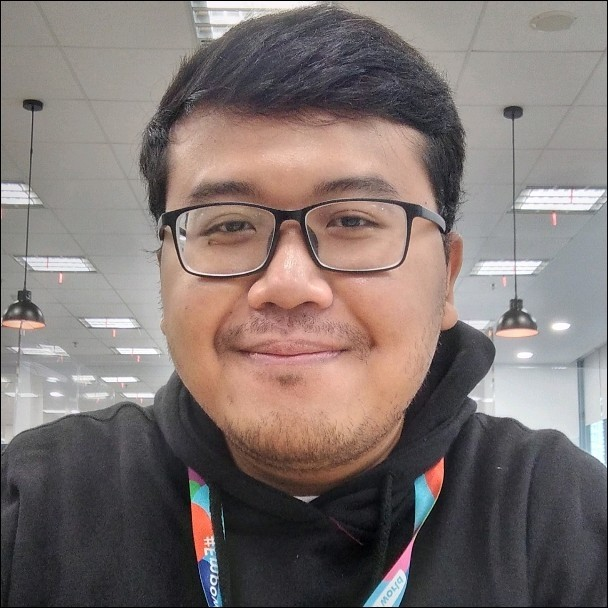
\includegraphics[height={120px}, width={90px}]{gambar/farhan}
\end{figure}

\noindent
\begin{tabular}{ll}
Nama & : Farhan Herdian Pradana \\
Tempat, Tanggal Lahir & : Jakarta, 28 Januari 2000 \\
Orang tua & : Dadang Budhi Herdiyana \& Sri Rejeki \\
Email & : farhan.herdia123@gmail.com
\end{tabular}

\section*{Pendidikan}
\begin{enumerate}
    \itemsep0em 
    \item SD Negeri Utan Kayu Utara 01 Pagi (2006-2012)
    \item SMP Negeri 7 Jakarta (2012-2015)
    \item SMA Negeri 22 Jakarta, Matematika dan Ilmu Alam (2015-2018)
    \item Universitas Negeri Jakarta, Ilmu Komputer (2018-)
\end{enumerate}

\section*{Pengalaman Kerja}
\begin{enumerate}
    \itemsep0em 
    \item Front End Developer Intern, \textbf{Lingotalk} (Juli - November, 2021)
    \item Android Engineer Intern, \textbf{Traveloka} (Februari - Juli 2022)
    \item Associate Software Engineer, \textbf{Blibli} (September 2022 - Sekarang)
\end{enumerate}
\end{document}